\chapter{Categorie, funtori, trasformazioni naturali}\label{chap_cat_fun_nat}
\section{Categorie}\label{sec_categorie}

Prima di dare una definizione formale di categoria, può essere d'aiuto raccogliere alcuni esempi concreti per orientare chi legge.

La nozione di categoria, che introdurremo in \ref{def_categ}, riuscirà a unificare due strutture matematiche apparentemente molto diverse tra loro:
\index{Monoide}
\begin{definition}\label{prelim_def_monoide}
	Un \emph{monoide} consiste di un insieme \(M\) dotato di
	\begin{itemize}
		\item un elemento \(e\in M\) (spesso denotato anche: \(1_M\) o semplicemente \(1\)), chiamato \emph{elemento neutro}, \emph{unità} o \emph{identità} (si noti che da ciò segue, indirettamente ma immediatamente, che \(M\) è un insieme \emph{non vuoto}),
		\item Un'operazione binaria \(M\times M\to M\), detta \emph{prodotto} o \emph{composizione}, e indicata con \((m,n)\mapsto m\cdot n\) o con simili simboli infissi come \(\star, \centerdot,\bullet\) eccetera,
	\end{itemize}
	che soddisfano le seguenti proprietà:
	\begin{itemize}
		\item \emph{Unitalità}: per ogni \(m\in M\), i prodotti \(m \cdot e\) ed \(e\cdot m\) sono uguali a \(m\);
		\item \emph{Associatività}: per ogni \(m,n,p\in M\), i prodotti \((m\cdot n)\cdot p\) ed \(m\cdot (n\cdot p)\) sono uguali.
	\end{itemize}
\end{definition}
\index{Poset}
\begin{definition}\label{prelim_def_preset}
	Un \emph{insieme preordinato} (o \emph{preordine} o \emph{preset}) consiste di un insieme \(P\) dotato di una relazione binaria \(\le\), solitamente indicata come un simbolo infisso \(x\le y\) per significare che \((x,y)\) è un elemento di \(\le\), che soddisfa le seguenti due proprietà:
	\begin{itemize}
		\item \emph{Riflessività}: per ogni \(x\in P\), si ha \(x\le x\);
		\item \emph{Transitività}: per ogni \(x,y,z\in P\), si ha che
		      \[(x\le y)\;\&\;(y\le z) \quad\implies\quad x\le z\]
	\end{itemize}
	Quando la relazione \(\le\) soddisfa anche la proprietà \emph{antisimmetrica}, cioè è tale per cui
	\[(x\le y)\;\&\;(y\le x) \quad\implies\quad x = y\]
	l'insieme \(P\), o meglio la coppia \((P,\le)\) si dice un insieme \emph{parzialmente ordinato} o \emph{poset}. La relazione \(\le\) in un poset si chiama un \emph{ordine parziale}.
\end{definition}
Dimostreremo in \ref{mon_sonocat} e in \ref{cat_sonopos} rispettivamente che ogni monoide è una categoria, e ogni insieme preordinato (e a fortiori, ogni insieme parzialmente ordinato) è una categoria. (Gli enunciati in questione renderanno più precise queste ultime affermazioni.)
\index{Categoria!--- degli insiemi finiti}
\begin{example}\label{protoex_finset}
	Un esempio naturale di categoria nasce considerando la classe \(\ctFin\) di tutti gli insiemi finiti \([n]\defeq \{1,\dots,n\}\) (con la convenzione che \([0]=\varnothing\) sia l'insieme vuoto), e le funzioni \(f : [n] \to [m]\) tra di loro. \`E evidente che non tutte tali funzioni sono componibili: una condizione necessaria --e sufficiente!-- affinché la composizione tra due funzioni \(f : [p] \to [q],g : [m] \to [n]\) tra insiemi finiti sia possibile è che il dominio dell'una coincida con il codominio dell'altra, ovvero che \(q=m\) e che le funzioni si possano `giustapporre' come
	\[\xymatrix{
			[p] \ar[r]^-f & [q] \ar[r]^-g & [r].
		}\]
	La composizione di funzioni \((f,g)\mapsto g\cmp f\) perciò è una operazione che ricorda quella di un monoide (per esempio, essa è associativa quando è definita) ma è appunto un'operazione \emph{parziale}, cioè non definita tra tutte le possibili coppie \((f,g)\) di funzioni tra insiemi finiti; quale che sia la struttura matematica che la classe degli insiemi finiti forma, perciò, essa non può essere un monoide. Un altro motivo per cui \(\ctFin\) non può essere un monoide è che l'identità per la composizione di funzioni non è unica come accade, invece, in ogni monoide: \emph{ogni} insieme finito \([n]\) ha una sua propria funzione identica \(\id_{[n]}\), e se \(f : [m]\to [n]\) con \(m\ne n\), si deve avere che \(f\cmp \id_{[m]}=f=\id_{[n]}\cmp f\) per funzioni identiche formalmente \emph{distinte}, sebbene definite `alla stessa maniera' da
	\[
		\begin{tikzcd}[row sep=0]
			{[n]} \ar{r}{\id_{[n]}} & {[n]} \\
			x \ar[mapsto]{r} & x
		\end{tikzcd}
		\qquad\mbox{e}\qquad
		\begin{tikzcd}[row sep=0]
			{[m]} \ar{r}{\id_{[m]}} & {[m]} \\
			y \ar[mapsto]{r} & y .
		\end{tikzcd}
	\]
	% \(\lambda x.x : [n]\to [n]\) e \(\lambda y.y : [m]\to [m]\). % non credo i lettori conoscano la notazione lambda, forse dovremmo introdurla

	La classe \(\ctFin\) formerà una \emph{categoria}, e per lo stesso motivo faranno altrettanto delle collezioni di oggetti matematici che esibiscono una struttura simile a quella di un monoide, ma sono più generali per motivi simili:
	\begin{itemize}
		\item \index{Categoria!---e di strutture algebriche} la classe \(\bbR\emdash\ctVect\) di tutti gli spazi vettoriali reali della forma \(\bbR^n\) per un \(n\) %\(n\ge 1\) 
		      naturale; non tutte le mappe lineari tra spazi vettoriali si possono comporre, e le applicazioni identiche sono tutte distinte; e più in generale,
		\item la classe di tutte le strutture algebriche di un dato tipo (gli insiemi, senza limite alla loro taglia; i gruppi, con gli omomorfismi di gruppo; gli spazi vettoriali, anche di dimensione infinita; gli spazi topologici, con le funzioni continue; eccetera).
	\end{itemize}
\end{example}
Una categoria sarà dunque, in prima approssimazione, una collezione di `oggetti' \(A,B,X,Y,\dots\), legati tra loro da delle relazioni o `funzioni astratte' \(f : X\to Y, g : A\to B\),\dots{} le quali potranno essere composte alla maniera delle funzioni. Questa intuizione è sufficiente per formulare la definizione, a cui deve però prima seguire una precisazione terminologica.
\begin{remark}
	\index{Classe}
	\index{Classe propria|see {Classe}}
	Abbiamo già utilizzato diverse volte la parola `classe': la definizione generale di categoria obbliga a farlo, dal momento che la collezione di tutte le strutture algebriche di un dato tipo è spesso `troppo grande per essere un insieme' (in un senso che formalizzeremo in dettaglio nell'Appendice \ref{fondamenti}); per il momento è sufficiente trattenere l'idea informale che una classe (o \emph{classe propria}) \(\ctC\) è una collezione di elementi che ha tutte le proprietà di un insieme, a parte quella di poter essere misurata da un numero cardinale.

	Ogni volta che è necessario, useremo costruzioni elementari che si possono fare sulle classi come se esse fossero insiemi: per esempio se \(\ctA,\ctB\) sono classi, è lecito costruire la classe prodotto \(\ctA\times\ctB\), e considerare \emph{funzioni tra classi} \(F : \ctA\fun\ctB\), cioè sottoclassi \(F\) del prodotto \(\ctA\times\ctB\) che sono funzionali: per ogni elemento \(A\) della classe \(\ctA\), esiste un unico elemento \(B\in\ctB\) con \((A,B)\in F\), questo elemento si denota \(FA\), e a tutti gli effetti \(F\) si comporta come una funzione. Di nuovo, il linguaggio preciso (il linguaggio \textsf{NBG} della teoria degli insiemi di von Neumann, Bernays e G\"odel) che formalizza queste costruzioni verrà esposto nell'appendice \ref{fondamenti}. Invitiamo il lettore interessato ad approfondire la questione nell'appendice, ma consigliamo di finire prima questo capitolo. Per ora, questa imprecisione iniziale non pregiudica né il rigore, né la comprensione degli argomenti che seguono.
\end{remark}
\index{Categoria}
\begin{definition}[Categoria]\label{def_categ}
	Una \emph{categoria} \(\ctC\) consiste dei seguenti dati:
	\begin{enumtag}{c}
		\item\label{c_1} una classe \(\ctC_0\) i cui elementi chiamiamo \emph{oggetti}, di solito indicati con lettere latine maiuscole: \(A\), \(B\), \(X\), \(Y\),\dots
		\item\label{c_2} una classe \(\ctC_1\) i cui elementi chiamiamo \emph{morfismi} o \emph{frecce}, di solito indicati con lettere latine minuscole: \(f,g,h\),\dots, \(u,v,w\)\dots
		\item\label{c_3} Ad ogni morfismo \(f\) corrispondono due oggetti \(\dom{f}\), \(\cod{f}\) chiamati \emph{dominio} e \emph{codominio}. Per denotare il fatto che \(f\) ha dominio \(X\in\ctC_0\) e codominio \(Y\in\ctC_0\), scriveremo \(f\colon X\to Y\), o in \emph{forma diagrammatica},
		\[\begin{tikzcd} X \ar[r, "f"] & Y. \end{tikzcd}\]
		\item\label{c_4} Ogni oggetto \(X\) ha un morfismo distinto \(\id_X\colon X\to X\) chiamato \emph{identità} o \emph{freccia identica}.
		\item\label{c_5} Per ogni coppia di morfismi \(f\colon X\to Y\) e \(g\colon Y\to Z\), cioè tali che \(\cod{f}=\dom{g}\), è dato un morfismo \(g\cmp f:X\to Z\) chiamato \emph{composizione di \(f\) e \(g\)}. Graficamente:
		\[
			\begin{tikzcd}
				X \ar{r}{f}
				\ar[rounded corners,out=-45, in=225]{rr}[swap]{g\cmp f}
				& Y \ar{r}{g} & Z \\
				&&
			\end{tikzcd}
		\]
		(Incidentalmente, osserviamo che \(\dom{g\cmp f}=\dom{f}\) e \(\cod{g\cmp f}=\cod{g}\).)
	\end{enumtag}
	A questi dati, chiediamo di soddisfare le seguenti proprietà:
	\begin{enumtag}{p}
		\item \label{cp_1} \emph{Unitalità}: per ogni morfismo \(f:X\to Y\), le composizioni \(f\cmp\id_X\) e \(\id_Y\cmp f\) sono uguali ad \(f\).
		\item \label{cp_2} \emph{Associatività}: dati oggetti \(X,Y,Z,W\) e morfismi \(f:X\to Y\), \(g:Y\to Z\) e \(h:Z\to W\), le composizioni \(h\cmp (g\cmp f)\) e \((h\cmp g)\cmp f\) sono uguali.
	\end{enumtag}
\end{definition}
\begin{notation}
	Dati due oggetti \(X\) e \(Y\), indichiamo con \(\Hom{\ctC}(X,Y)\) la classe di morfismi da \(X\) a \(Y\). Altre notazioni, come \(\mathrm{Hom}(X,Y)\) o \(\mathrm{Hom}_\ctC(X,Y)\), sono ugualmente comuni, e motivate dal fatto che le frecce di una categoria astraggono la nozione di \emph{omomorfismo} tra insiemi strutturati (si veda \ref{ex_cat_monoidi} e più in generale l'esempio \ref{ex_cat_sigma_strutture}). Questa notazione renderà chiara quella in \ref{ex_hom_funtore} per i funtori hom.
	% TODO: mettere in una definizione sola "tutte" le categorie di strutture algebriche.
\end{notation}
\begin{remark}\label{cor_def_categ}
	Si osservi che dalla definizione appena data discendono due corollari:
	\begin{itemize}
		\item Le classi \(\Hom{\ctC}(X,Y)\) al variare di \((X,Y)\in\ctC_0\times\ctC_0\) sono tutte disgiunte, perché la corrispondenza \(\ctC_1 \to \ctC_0\times\ctC_0\) che manda \(f\) nella coppia \((\dom{f},\cod{f})\) è una funzione (e allora la sua `fibra' sopra \((X,Y)\) è proprio \(\Hom{\ctC}(X,Y)\), disgiunto da \(\Hom{\ctC}(X',Y')\));
		\item come conseguenza immediata, se \(X\ne X'\) sono oggetti diversi, le identità \(\id_X,\id_{X'}\) sono morfismi diversi: si può cioè pensare la corrispondenza \(X\mapsto \id_X : \ctC_0\to\ctC_1\) come una funzione \emph{iniettiva} tra classi;
		\item la composizione consta di una funzione \emph{parziale}
		      \[\xymatrix{\_\cmp\_ : \ctC_1 \times \ctC_1 \ar[r] & \ctC_1}\]
		      il cui dominio è la sotto-classe \(\sum_{XYZ} \{ X \xrightarrow f Y \xrightarrow g Z \}\) dei morfismi \emph{contigui} o componibili. Dato che i vari \(\ctC(X,Y)\) sono a due a due disgiunti, la composizione \(\_\cmp\_\) si `decompone' in una classe di funzioni
		      \[\xymatrix{\_\cmp_{XZ}^Y\_ : \ctC(Y,Z)\times\ctC(X,Y) \ar[r] & \ctC(X,Z)}\]
		      dove ciascuna manda \(( X \xrightarrow f Y, Y \xrightarrow g Z )\) in \(g\cmp f\) (praticamente sempre, si sottintende il dominio particolare di \(\_\cmp_{XZ}^Y\_\)).
	\end{itemize}
\end{remark}
\begin{definition}[Categoria piccola, categoria localmente piccola]
	\index{Categoria!--- piccola}
	\index{Categoria!--- loc. piccola}
	Quando la classe \(\ctC_1\) è un insieme, come conseguenza della seconda osservazione fatta, è un insieme anche \(\ctC_0\): in tal caso chiamiamo la categoria \(\ctC\) \emph{piccola}: le categorie \(\ctFin\) e \(\bbR\emdash\ctVect\) definite sopra sono piccole, perché abbiamo limitato enormemente la loro classe di oggetti; non abbiamo considerato \emph{tutti} gli insiemi finiti, ma solo quelli della forma \(\{1,\dots,n\}\). Una categoria che non è piccola si dice \emph{grande}, \emph{larga} o simili.

	Invece, \(\ctC\) si dice \emph{localmente piccola} se dati ogni due oggetti \(X\) e \(Y\), la classe \(\Hom{\ctC}(X,Y)\) di morfismi da \(X\) a \(Y\) è un insieme. La categoria di \emph{tutti} gli insiemi finiti non è, strettamente parlando, piccola (perché c'è una classe propria anche solo di insiemi con un singolo elemento: \(\{\varnothing\},\{\{\varnothing\}\}, \{\{\{\varnothing\}\}\}\), eccetera), ma è localmente piccola, perché fissati due insiemi \(X,Y\), la collezione delle funzioni \(f : X\to Y\) è contenuta in \(2^{X\times Y}\), e quest'ultimo è un insieme (per assioma).
\end{definition}
\begin{remark}
	Gli assiomi di categoria non impediscono di costruire `categorie' dove \(\ctC_0\) è un insieme (per esempio, finito) e dove alcuni o tutti \(\Hom{\ctC}(X,Y)\) sono classi proprie; queste costruzioni sono però relativamente innaturali, e non ne parleremo mai. In effetti, non parleremo mai nemmeno di categorie grandi che non sono localmente piccole (ne risentirebbe irrimediabilmente il capitolo 4 del libro, e molti altri risultati). Perciò, da ora in poi adottiamo la convenzione che \emph{categoria}, se non specifichiamo altro, significhi sempre \emph{categoria localmente piccola}. Alternative a questa maniera di ragionare sono possibili, ma non porremo mai una particolare attenzione alla questione.
\end{remark}
Concludiamo con un lemma apparentemente banale, ma che sarà utile in seguito (precisamente, nella dimostrazione di \ref{cat_sonomon}).
\begin{lemma}\label{lem_end_monoide}
	Sia \(\ctC\) una categoria, \(A\in\ctC_0\) un suo oggetto; allora \(M=\Hom{\ctC}(A,A)\) è un monoide, con l'identità \(\id_A\) come elemento neutro e la composizione \(\cmp\) come prodotto.
\end{lemma}
\begin{proof}
	La composizione è un'operazione associativa
	\[\begin{tikzcd}
			M\times M \ar[r, "\cmp"] & M
		\end{tikzcd}\]
	per \ref{cp_2}, e il fatto che \(f\cmp \id_A=f=\id_A\cmp f\) segue da \ref{cp_1}, in \ref{def_categ}.
\end{proof}
Nel resto della sezione raccogliamo alcuni esempi classici di categorie, e nella successiva inizieremo a `costruire categorie nuove dalle vecchie', cioè a definire il \emph{prodotto} \(\ctC\times\ctD\) (si veda \ref{def_cat_prodotto}) e la \emph{somma} \(\ctC+\ctD\) di due categorie date in \ref{def_cat_somma}, le categorie \emph{comma} \(\ctC/X\) e \emph{co-comma} \(X/\ctC\) sopra un oggetto \(X\in\ctC_0\) in \ref{def_cat_cocomma}, la categoria \emph{opposta} \(\ctC^\op\) di \(\ctC\) in \ref{def_cat_opp}, e molte altre.

La dicotomia essenziale che chi legge dovrebbe apprezzare è questa:
\begin{itemize}
	\item le categorie sono strutture ideate per raccogliere una totalità di oggetti matematici di un dato tipo (tutti i gruppi, tutti gli spazi topologici, ecc.) in una classe \(\ctC\) (in \emph{due} classi: gli oggetti e i morfismi) e studiarne le proprietà globali: le categorie (grandi) quindi sono `universi del discorso matematico': questo punto di vista si apprezza nella \autoref{ssec:categorie_universi} e particolarmente in \ref{ex_cat_sigma_strutture} e in \ref{ex_cat_top}.
	\item D'altra parte le categorie sono anche delle strutture matematiche a sé stanti, modellate sulla nozione elementare di \emph{multigrafo diretto} (si veda \ref{ex_cat_libera}): le categorie (piccole) quindi sono esse stesse degli oggetti matematici che possiamo studiare alla stregua di ogni altro oggetto matematico (e raccogliere in una loro totalità: ma questo discorso sarà approfondito solo molto più tardi, si veda \ref{ex_cat_cat}). Questo punto di vista si apprezza particolarmente nella \autoref{ssec:categorie_strutture}.
\end{itemize}
Si può imparare la teoria delle categorie in modo proficuo solo abbracciando \emph{entrambi} questi punti di vista, e ciò perché un dato ambito della matematica si occupa o `vive' in una (o più) categorie. Per esempio, l'algebra lineare studia le categorie \(\bbF\emdash\ctVect\) di spazi vettoriali, eventualmente su diversi campi di base (come \(\bbQ,\bbR,\bbC\), o un campo finito). La topologia generale studia le categorie di \emph{spazi topologici} (e i morfismi funzioni continue), mentre la topologia differenziale si restringe alla categoria i cui oggetti sono \emph{varietà} (e i morfismi funzioni differenziabili), oppure studia particolari categorie di strutture ordinate (perché l'insieme degli aperti di uno spazio topologico \(X\) con una topologia \(\tau \subseteq 2^X\) forma, con le operazioni di unione e intersezione, una struttura algebrica detta \emph{algebra di Heyting}, si veda \cite{Esakia2019}).

D'altra parte l'analisi funzionale studia quegli spazi \emph{vettoriali} (di dimensione infinita) che sono dotati di una \emph{topologia} metrizzabile (e determinata da un filtro di intorni dello zero), ed eventualmente di un prodotto scalare; la teoria della rappresentazione studia certi omomorfismi in un gruppo di matrici, o le proprietà \emph{topologiche-differenziali} di questi gruppi di matrici (il gruppo ortogonale speciale, il gruppo dei quaternioni di norma 1, ecc.). Per comprendere queste strutture è spesso necessario spostarsi di categoria in categoria.

La seconda di queste osservazioni non è meno importante: porterà alla definizione di funtore in \ref{def_funtore} come \emph{omomorfismo tra categorie}, alla definizione di \emph{diagramma} in \ref{def_diagramma} come immagine di una categoria piccola in una categoria, non necessariamente piccola, e alla definizione di trasformazione naturale in \ref{sec_tnat}, vista come \emph{omomorfismo tra funtori}.
\section{Esempi di categorie nella pratica matematica}\label{sec_esempi_cats}
Iniziamo ora a dare degli esempi di categorie piccole partendo dall'esempio più semplice, anche quello più banale.
\subsection{Categorie come forme}\label{ssec:categorie_forme}
\index{Categoria!--- vuota}
\begin{example}\label{ex_cat_vuota}
	La \emph{categoria vuota} o \emph{categoria iniziale} \(\ctInit\) non ha oggetti né morfismi. Più formalmente, \(\ctC_0,\ctC_1\) sono le classi vuote, e non è necessario specificare altra struttura per soddisfare (vacuamente) tutti gli assiomi di categoria.
\end{example}
\index{Categoria!--- terminale}
\begin{example}\label{ex_cat_term}
	La \emph{categoria terminale} \(\ctTerm\) ha un solo oggetto \(\bullet\), e un unico morfismo \(\id_\bullet : \bullet\to\bullet\) che fa da identità. Chiaramente, non si può fare altro che porre \(\id_\bullet\cmp\id_\bullet=\id_\bullet\), e tutti gli assiomi di categoria sono soddisfatti.
\end{example}
\index{Categoria!--- discreta}
\`E sempre possibile dotare un insieme \(A\) della topologia discreta (o `massimale'), dove ogni sottoinsieme \(U\) di \(A\) è aperto, e della topologia indiscreta (o `minimale'), dove solo \(\varnothing\) e \(A\) sono aperti. Similmente, esistono due maniere, massimale e minimale, di considerare un insieme\footnote{Riguardo al problema se sia possibile dotare una classe propria della struttura di categoria discreta, la questione \emph{sembra} banale, ma in realtà tutt'altro che semplice da discutere: sebbene non ci sia alcun apparente problema ad assumere l'esistenza di classi proprie discrete, queste spesso vengono proibite \emph{ab imis} assumendo un assioma a parte in aggiunta ai soliti della teoria degli insiemi/classi, detto \emph{principio di Vop\v enka}: questo assioma afferma, precisamente, che non esistono sottoclassi proprie discrete nella classe propria di tutti gli insiemi.} \(A\) una categoria.
\begin{example}\label{ex_cat_discreta}
	Dato un insieme \(A\), la \emph{categoria discreta} su \(A\), denotata \(A^\delta\), ha per oggetti gli elementi \(a\in A\), un unico morfismo identico \(\id_a : a\to a\) per ogni \(a\), e nessun altro. La composizione è forzata a essere definita solamente tra identità, nel modo più ovvio possibile, e tutti gli assiomi di categoria sono ovviamente soddisfatti.
\end{example}
\begin{example}\label{ex_cat_codiscreta}
	Dato un insieme \(A\), la \emph{categoria codiscreta} su \(A\), denotata \(A^\chi\) ha per oggetti gli elementi \(a\in A\), per ogni coppia di oggetti \(a,a'\in A\) un unico morfismo \(u_{aa'}:a\to a'\), e la composizione è definita da \(u_{a'a''}\cmp u_{aa'}=u_{aa''}\) (in particolare, da questo segue che esiste un unico elemento \(\id_a=u_{aa}\in A^\chi(a,a)\)).
\end{example}
Alcune categorie che è spesso utile considerare si rappresentano mediante dei grafi:
\index{Categoria!--- freccia generica}
\begin{example}\label{ex_cat_freccia}
	La categoria `freccia generica' ha due oggetti \(0,1\) e un unico morfismo non identico \(u : 0\to 1\) (che di solito non ha nome). La composizione è forzata a essere definita solamente tra le identità ed \(u\), nell'unico modo ovvio, e tutti gli assiomi di categoria sono banalmente soddisfatti.
\end{example}
\index{Categoria!--- catena generica}
\begin{example}\label{ex_cat_catena}
	Più in generale, la categoria \(\Delta[n]\) detta `catena generica di lunghezza \(n+1\)' è definita come segue:
	\begin{itemize}
		\item gli oggetti di \(\Delta[n]\) sono gli elementi di \(\{0,\dots,n\}\) (ci sono quindi \(n+1\) oggetti, per ogni \(n\ge 1\));\footnote{A volte è utile adottare la convenzione per cui quando \(n=-1\), l'insieme \(\{0,\dots,n\}\) è vuoto, e quindi la categoria `catena di lunghezza \(0\)' è la categoria vuota \(\ctInit\) di \ref{ex_cat_vuota}.}
		\item C'è un unico morfismo \(i\to j\) in \(\Delta[n]\) se e solo se \(i\le j\), di modo che esista un unico morfismo \(i\to i\) (l'identità) per ogni \(i\in\{0,\dots,n\}\), e un unico morfismo \(i\to i+1\) per \(i\in\{0,\dots,n-1\}\); in particolare l'unico morfismo \(i\to j\) è ottenuto dalla composizione
		      \[i\to i+1\to\dots\to j\]
	\end{itemize}
	Le categorie \(\Delta[n]\) per \(=0,1,2,3\) sono rappresentate in figura \ref{fig:le_delta}.
	\begin{figure}[h]
		\begin{center}
			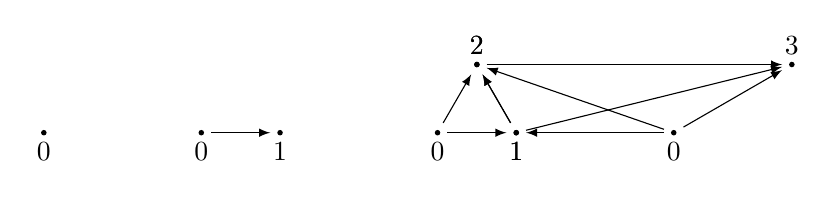
\begin{tikzpicture}
				\node (0) at (0,0) {};
				\fill (0,0) circle (1pt) node[below] {\(0\)};
				%--
				\fill (2,0) circle (1pt) node[below] {\(0\)};
				\node (0') at (2,0) {};
				\fill (3,0) circle (1pt) node[below] {\(1\)};
				\node (1') at (3,0) {};
				\draw[-latex] (0') -- (1');
				%--
				\fill (5,0) circle (1pt) node[below] {\(0\)};
				\node (0'') at (5,0) {};
				\fill (5.5,0.866) circle (1pt) node[above] {\(2\)};
				\node (2'') at (5.5,0.866) {};
				\fill (6,0) circle (1pt) node[below] {\(1\)};
				\node (1'') at (6,0) {};
				\draw[-latex] (0'') -- (1'');
				\draw[-latex] (1'') -- (2'');
				\draw[-latex] (0'') -- (2'');
				%--
				\fill (8,0) circle (1pt) node[below] {\(0\)};
				\node (0'') at (8,0) {};
				\fill (5.5,0.866) circle (1pt) node[above] {\(2\)};
				\node (2'') at (5.5,0.866) {};
				\fill (6,0) circle (1pt) node[below] {\(1\)};
				\node (1'') at (6,0) {};
				\fill (9.5,0.866) circle (1pt) node[above] {\(3\)};
				\node (3'') at (9.5,0.866) {};
				\draw[-latex] (0'') -- (1'');
				\draw[-latex] (1'') -- (2'');
				\draw[-latex] (0'') -- (2'');
				\draw[-latex] (2'') -- (3'');
				\draw[-latex] (1'') -- (3'');
				\draw[-latex] (0'') -- (3'');
			\end{tikzpicture}
		\end{center}
		\caption{Le categorie \(\Delta[0], \dots,\Delta[3]\). Si noti che non abbiamo rappresentato le frecce identiche dei vari oggetti, e che la struttura di categoria che risulta è completamente determinata dalla struttura di grafo diretto. Ovviamente, \(\Delta[0]\) è la categoria terminale di \ref{ex_cat_term}, \(\Delta[1]\) è la freccia generica di \ref{ex_cat_freccia}. La categoria \(\Delta[n]\) spesso si chiama un \(n\)-\emph{simplesso}.}
		\label{fig:le_delta}
	\end{figure}
\end{example}
\index{Categoria!--- doppia freccia generica}
\begin{example}\label{ex_cat_doppiafreccia}
	La categoria `doppia freccia generica' ha due oggetti \(0,1\) ed esattamente due morfismi non identici e paralleli \(s,t : 0\to 1\)%
	%;anche in questo caso, tali morfismi di solito non hanno nome % ce l'hanno: s e t
	. La composizione è definita, ancora una volta, nell'unico modo ovvio, chiedendo che \(x\cmp \id_0=x=\id_1\cmp x\) per \(x\in\{s,t\}\).

	La doppia freccia è la `forma generica' di un grafo diretto (si veda \ref{ex_cat_libera}), dato che una coppia di funzioni \(s,t: X_1 \rightrightarrows X_0\) tra due insiemi consta precisamente di un digrafo che ha \(X_0\) per insieme dei vertici e \(X_1\) per insieme dei lati.
\end{example}
\index{Categoria!--- quadrato commutativo generico}
\begin{example}\label{ex_quadcuboncubo}
	La categoria `quadrato commutativo generico' \(P[2]\) ha 4 oggetti
	\[\{(00),(10),(01),(11)\} \]
	e un morfismo \((ij)\to(kl)\) se e solo se \(i\le k\) e \(j\le l\); rappresentata graficamente, si tratta della categoria
	\[\begin{tikzcd}
			(00) \ar[r]\ar[d]\ar[dr]& (10)\ar[d] \\
			(01) \ar[r]& (11)
		\end{tikzcd}\]
	La composizione è forzata a essere definita cosicché la composizione \((00)\to (01)\to (11)\) sia uguale alla composizione \((00)\to (10)\to (11)\), e quindi la categoria \(P[2]\) rappresenta la forma generica di un quadrato commutativo.

	Si noti che \(P[2]\) è un insieme ordinato, e precisamente l'insieme dei sottoinsiemi di un insieme con due elementi \(\{a,b\}\); in tal senso \((ij)\) rappresenta la funzione caratteristica \(\chi_U : \{a,b\}\to \{0,1\}\) di un sottoinsieme \(U\subseteq \{a,b\}\), nel senso che ad esempio \((10)=\{a\}, (00)=\varnothing\), eccetera. Si osservi anche che \(P[2]\) è l'insieme parzialmente ordinato \(\{0\le 1\}\times \{0\le 1\}\), dotato dell'\emph{ordine prodotto} (si veda \ref{ord_sonocat} e \ref{cat_sonopos}).

	Quindi possiamo definire induttivamente
	\[P[0] = \Delta[0], \qquad P[n+1] = P[n]\times \Delta[1]\]
	o (equivalentemente, nel senso che questa seconda definizione dà per ogni \(n\ge 0\) un \(P'[n]\) isomorfo a \(P[n]\) come insieme ordinato) \(P'[n] = 2^{\{1,\dots,n\}}\), cosicché \(P[n]\) è il `cubo commutativo \(n\)-dimensionale generico': alcune \(P[n]\) per \(n=0,1,2,3\) sono raffigurate in \ref{fig_n_cubo}.
\end{example}
\begin{figure}[h]
	\begin{center}
		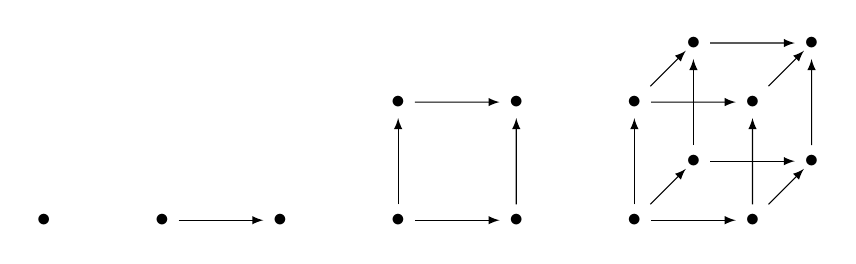
\begin{tikzpicture}[scale=1.5]
			\node (empty) at (-1,0) {\(\bullet\)};
			%
			\node (0) at (0,0) {\(\bullet\)};
			\node (1) at (1,0) {\(\bullet\)};
			\draw[-latex] (0) -- (1);
			\begin{scope}[xshift=2cm]
				\node (00) at (0,0) {\(\bullet\)};
				\node (10) at (1,0) {\(\bullet\)};
				\node (01) at (0,1) {\(\bullet\)};
				\node (11) at (1,1) {\(\bullet\)};
				\draw[-latex] (00) -- (10);
				\draw[-latex] (10) -- (11);
				\draw[-latex] (00) -- (01);
				\draw[-latex] (01) -- (11);
			\end{scope}
			\begin{scope}[xshift=4cm]
				\node (00) at (0,0) {\(\bullet\)};
				\node (10) at (1,0) {\(\bullet\)};
				\node (01) at (0,1) {\(\bullet\)};
				\node (11) at (1,1) {\(\bullet\)};
				\draw[-latex] (00) -- (10);
				\draw[-latex] (10) -- (11);
				\draw[-latex] (00) -- (01);
				\draw[-latex] (01) -- (11);
			\end{scope}
			\begin{scope}[xshift=4.5cm,yshift=.5cm]
				\node (00') at (0,0) {\(\bullet\)};
				\node (10') at (1,0) {\(\bullet\)};
				\node (01') at (0,1) {\(\bullet\)};
				\node (11') at (1,1) {\(\bullet\)};
				\draw[-latex] (00') -- (10');
				\draw[-latex] (10') -- (11');
				\draw[-latex] (00') -- (01');
				\draw[-latex] (01') -- (11');
			\end{scope}
			\draw[-latex, shorten >=-.35pc] (00) -- (00');
			\draw[-latex, shorten >=-.35pc] (01) -- (01');
			\draw[-latex, shorten >=-.35pc] (10) -- (10');
			\draw[-latex, shorten >=-.35pc] (11) -- (11');
		\end{tikzpicture}
	\end{center}
	\caption{Le categorie \(P[n]\) per \(n=0,1,2,3\). La categoria \(P[n]\) si chiama un \(n\)-\emph{cubo}.}
	\label{fig_n_cubo}
\end{figure}
\index{Categoria!--- span generico}
\index{Categoria!--- cospan generico|see {span generico}}
\begin{example}[Span e cospan generici]\label{ex_spancospan}
	La categoria `span generico' \(\Lambda^2_0\) ha tre oggetti \(0,1,2\) e due morfismi non identici. Si raffigura come segue:
	\[\begin{tikzcd}
			1 & 0 \ar[r]\ar[l] & 2
		\end{tikzcd}\]
	La composizione è definita solamente quando almeno una delle due frecce è identica, ed è forzata da questo fatto.

	Dualmente, la categoria `cospan generico' \(\Lambda^2_2\) ha tre oggetti \(0,1,2\) ma i due morfismi non identici puntano verso \(2\) invece che uscire da \(0\):
	\[\begin{tikzcd}
			0\ar[r] & 2 & 1\ar[l]
		\end{tikzcd}\]
	Di nuovo, la composizione è definita solamente quando almeno una delle due frecce è identica.

	Si noti che \(\Lambda^2_2\) si ottiene da \(\Delta[2]\) `rimuovendo la freccia \(0\to 1\)', e analogamente \(\Lambda^2_0\) si ottiene rimuovendo la freccia \(1\to 2\).

	Più in generale, sia \(S\) un insieme; la categoria `\(S\)-span generico' \(S^\lhd\) è definita come segue:
	\begin{itemize}
		\item gli oggetti di \(S^\lhd\) sono gli elementi di \(S^+ := S\cup \{-\infty\}\);
		\item esiste un unico morfismo \(f_s : -\infty\to s\), per ogni \(s\in S\).
	\end{itemize}
	La composizione è ancora una volta definita solamente quando almeno una delle due frecce è identica. Questo definisce una categoria in cui da un oggetto chiamato `\(-\infty\)' spiccano tante frecce \(f_s\) quanti sono gli elementi di \(S\).

	Dualmente, definiamo la categoria `\(S\)-cospan generico' \(S^\rhd\) come segue:
	\begin{itemize}
		\item gli oggetti di \(S^\rhd\) sono gli elementi di \(S^+ := S\cup \{+\infty\}\);
		\item esiste un unico morfismo \(f_s : s\to+\infty\), per ogni \(s\in S\).
	\end{itemize}
	La composizione è ancora una volta definita solamente quando almeno una delle due frecce è identica. Questo definisce una categoria in cui verso un oggetto chiamato `\(\infty\)' puntano tante frecce \(f_s\) quanti sono gli elementi di \(S\).

	Si noti che \(\Lambda^2_0=\{1,2\}^\lhd\) e \(\Lambda^2_2=\{0,1\}^\rhd\).
\end{example}
\index{Categoria!--- libera}
Questi ultimi esempi lasciano supporre che \emph{ogni} grafo \(\ctG\), fatto di un insieme di vertici (o `oggetti') \(V\) e di un insieme di lati (o `morfismi') \(E\) generi una categoria \(F\ctG\). \`E effettivamente così, e la seguente costruzione in forma di esempio formalizza questa idea.
\index{Grafo}
\begin{example}\label{ex_cat_libera}
	Dato un grafo (o più propriamente, un \emph{multidigrafo}, ossia una coppia di insiemi \(E,V\) dotati di due funzioni \(s,t : E\rightrightarrows V\) che associano ad ogni \emph{lato} \(e\in E\) una coppia ordinata di \emph{vertici} \(s(e),t(e)\in V\) detti il suo dominio o \emph{source} e il suo codominio o \emph{target}, si veda \ref{ex_cat_grafi}) \(\ctG\) possiamo definire la \emph{categoria libera} \(F\ctG\) su \(\ctG\) come segue:
	\begin{itemize}
		\item gli oggetti di \(F\ctG\) sono esattamente gli elementi di \(V\);
		\item fissati due vertici \(u,v\in V\), i morfismi \(u\to v\) sono l'insieme
		      \[\sum_{n=0}^\infty E(u,x_1)\times E(x_1,x_2)\times\dots\times E(x_n,v)\]
		      di tutte le sequenze ordinate e finite di lati
		      \[ [\tup en;] : u \xto{e_1} x_1 \xto{e_2} x_2\xto{e_3} \dots\xto{e_{n-1}} x_{n-1}\xto{e_n} v\]
		      con la convenzione che se \(u=v\) ed \(n=0\) la sequenza vuota si interpreta come un laccio `banale' \(\emptyList_u : u\to u\), e usando la notazione, ovvia, \(E(x,y)\subseteq E\) per denotare i lati di source \(x\) e target \(y\).
	\end{itemize}
	La composizione di due sequenze \([\tup fm;]\) e \([\tup en;]\) è data dalla loro \emph{concatenazione}, ossia dalla operazione
	\[[\tup fm;]\cmp[\tup en;] = [\tup fm;;\tup en;].\]
	Quando è definita, questa operazione è, evidentemente, associativa, e la sequenza vuota soddisfa la condizione di unitalità \ref{cp_1} nella \ref{def_categ}.
\end{example}
Dopo questa digressione veniamo a due esempi più elaborati, ma molto `concreti', di categorie dove gli oggetti sono numeri naturali:
\index{Categoria!--- dei circuiti}
\begin{example}[La categoria dei circuiti digitali]\label{ex_cat_circuiti}
	La categoria \(\ctCirc\) ha
	\begin{itemize}
		\item per oggetti i numeri naturali \(0,1,2,\dots\);
		\item l'insieme dei morfismi \(\ctCirc(m,n)\) consiste dell'insieme delle funzioni \(\bbB^n\to \bbB^m\), dove \(\bbB=\{0,1\}\) è l'insieme dei \emph{Booleani}\footnote{L'insieme \(\bbB\) può essere interpretato come: l'insieme degli interi positivi modulo 2, l'insieme degli stati di un singolo bit di informazione; l'insieme \{sì, no\} delle risposte a una domanda; l'insieme \(\{-1,1\}\) dei \emph{segni} assunti dagli elementi dell'immagine di una funzione reale, l'insieme \{acceso, spento\} degli stati di un interruttore, eccetera.} e \(\bbB^0\defeq \{*\}, \bbB^{n+1}\defeq \bbB^n\times \bbB\) sono i prodotti cartesiani iterati di \(\bbB\) con sé stesso.
	\end{itemize}
	Si noti che ogni funzione Booleana \(f : \bbB^n\to\bbB^m\) risulta dal `prodotto' di \(m\) funzioni Booleane \emph{semplici} \(f_1,\dots,f_m : \bbB^n\to\bbB\), di modo che
	\[f(\tup xn,)=(f_1(\tup xn,),\dots,f_m(\tup xn,))\]
	Tra le funzioni Booleane semplici ci sono certamente le proiezioni canoniche \(\pi_i : \bbB^n\to\bbB :(\tup xn,)\mapsto x_i\), ma anche le mappe diagonali \(\Delta_m:\bbB\to\bbB^m\) definite da
	\[\Delta_m : x\mapsto (x,\dots,x)\quad m\text{ volte}\]
	Sull'insieme dei Booleani è possibile definire le operazioni logiche elementari di disgiunzione, congiunzione e negazione, che rappresentiamo graficamente con i seguenti diagrammi (noti a qualsiasi ingegnere elettronico)
	\[\begin{circuitikz}
			\node[xshift=-4cm, or port, fill=gray!10] (4,0) (or) {\(\lor\)};
			\node[and port, fill=gray!10] (0,0) (and) {\(\land\)};
			\node[xshift=3cm, not port, fill=gray!10] (0,0) (not) {\(\lnot\)};
			\node[below=.15cm of or ] (z1) {\(\_\lor\_ : \bbB^2\to\bbB\)};
			\node[below=.15cm of and] (z3) {\(\_\land\_ : \bbB^2\to\bbB\)};
			\node[below=.15cm of not] (z2) {\(\_\lnot : \bbB\to\bbB\)};
		\end{circuitikz}\]
\end{example}
Vale il seguente teorema:
\begin{theorem}
	\Todo{qualcosa che dovrebbe essere nel libro di Walters \cite{Walters1992}, da cui ho preso questo esempio}
\end{theorem}
\index{Categoria!--- dei diagrammi di flusso}
\begin{example}[La categoria dei diagrammi di flusso]\label{ex_cat_flusso}
	La categoria \(\ctFlux\) è definita come segue:
	\begin{itemize}
		\item gli oggetti di \(\ctFlux\) sono i numeri naturali \(0,1,2,\dots\);
		\item l'insieme dei morfismi \(\ctFlux(n,m)\) consiste dell'insieme delle funzioni \(\bbR^n\to \bbR^m\), dove \(\bbR\) consta dell'usuale insieme dei numeri reali, e \(\bbR^n = \bbR\times\dots\times\bbR\) è il prodotto cartesiano iterato di \(\bbR\) con sé stesso.
	\end{itemize}
	\Todo{...}
\end{example}
\subsection{Categorie come universi}\label{ssec:categorie_universi}
Proseguiamo con degli esempi di categorie grandi, che giustificano l'intuizione per le categorie come universi del discorso.
\index{Categoria!--- delle relazioni}
\begin{example}[Insiemi e relazioni]\label{ex_cat_rels}
	La categoria \(\ctRel\) ha
	\begin{itemize}
		\item per oggetti gli insiemi, denotati con le lettere \(A,B,C,\dots\);
		\item per morfismi da \(A\) verso \(B\) tutte le \emph{relazioni} \(R\subseteq A\times B\), ossia i sottoinsiemi del prodotto cartesiano \(A\times B\).
	\end{itemize}
	Una relazione \(R\subseteq A\times B\) e una relazione \(S\subseteq B\times C\) si compongono nella relazione \(S\cmp R\) definita da
	\[(a,c)\in S\cmp R\iff \exists b\in B ((a,b)\in R)\land ((b,c)\in S).\]
	Con questa definizione, si può mostrare che \(T\cmp(S\cmp R)=(T\cmp S)\cmp R\) e che la relazione diagonale \(\{(a,a)\mid a\in A\}\subseteq A\times A\) (ovvero la relazione \(a\,\Delta\,a'\iff a=a'\)) funge da elemento identità per la composizione così definita.
\end{example}
Nell'esempio appena fatto, l'ordine in cui si scrivono i fattori di un prodotto cartesiano è importante, perché se \(R : A\to B\) è una relazione, vogliamo che \(A\) ne sia il dominio, e \(B\) il codominio. \`E però vero che gli insiemi \(A\times B\) e \(B\times A\) sono in biiezione canonica, e quindi si potrebbe pensare di definire una categoria \(\ctRel'\) con gli stessi oggetti di \(\ctRel\), ma con morfismi da \(A\) verso \(B\) le relazioni \(R\subseteq B\times A\). In effetti, questa è la categoria opposta \(\ctRel^\op\) di \(\ctRel\) (si veda \ref{def_cat_opp}), e tra \(\ctRel^\op\) e \(\ctRel\) esiste una identificazione canonica.
\index{Categoria!--- degli insiemi}
\index{Categoria!--- degli insiemi finiti|see {--- degli insiemi}}
\begin{remark}\label{klext_delle_relazioni}
	Ogni relazione \(R : A\to B\) induce una funzione \(R^* : 2^B\to 2^A\) nel modo che segue: un sottoinsieme \(U\subseteq B\) viene mandato in \(R^*U:=\{x\in A\mid \forall u\in U.(x,u)\in R\}\). In effetti, esiste una analoga funzione \(R_* : 2^A\to 2^B\), definita da \((V\subseteq A) \mapsto R_*V:= \{y\in B\mid \forall v\in V.(v,y)\in R\}\), e tra le due funzioni \(R^*, R_*\) sussiste la relazione
	\[V\subseteq R^*U \iff U\subseteq R_*V\label{aggiunti_in_disguise}\]
	In \ref{} questo sarà un esempio elementare di una nozione importante, quella di \emph{aggiunzione} tra due categorie, affrontata per esteso nel capitolo \ref{cap:aggiunti}.
\end{remark}
\begin{example}[Insiemi e funzioni]\label{ex_cat_insiemi}
	La categoria \(\ctSet\) ha
	\begin{itemize}
		\item per oggetti gli insiemi, denotati con le lettere \(A,B,C\dots\);
		\item per morfismi da \(A\) vero \(B\) tutte le funzioni \(f : A\to B\), ossia tutte le relazioni \(F\subseteq A\times B\) con la proprietà che per ogni \(a\in A\) esiste un unico \(b\in B\) tale che \((a,b)\in F\) o, più formalmente, \(F\cap(\{a\}\times B)\) è un singoletto; l'elemento \(b\) in questione si denota \(f(a)\) o \(fa\) e l'insieme \(F = \{(a,fa)\mid a\in A\}\) è il \emph{grafico} o \emph{supporto} della funzione. Queste relazioni sono \emph{totali} (perché sono definite sull'intero dominio \(A\)) e \emph{a valore singolo}.
	\end{itemize}
	Due funzioni \(f : A\to B\), \(g : B\to C\) si compongono alla maniera delle relazioni (e la composizione è ancora una funzione, poiché l'intersezione \((G\cmp F)\cap (\{a\}\times C)\) consta del singoletto \(\{g(fa)\}\)).

	La relazione diagonale è infine la funzione identica.
\end{example}
Evidentemente, possiamo restringerci a considerare la categoria dei soli insiemi \emph{finiti} (così come la categoria \(\ctFRel\) delle relazioni tra insiemi finiti, che la contiene propriamente). Questo è il primo degli esempi motivanti fatti ad inizio capitolo, e in un senso evidente (che sarà precisato dalla definizione \ref{def_subcat}), \(\ctFRel\) è una \emph{sottocategoria} di \(\ctRel\) (e \(\ctFin\) è una sottocategoria di \(\ctSet\), che a sua volta è una sottocategoria di \(\ctRel\), sebbene in un modo non completamente banale).
\index{Categoria!--- delle matrici}
\begin{example}[Categoria delle matrici in \(\bbF\)]\label{ex_cat_matrici}
	La categoria \(\bbF\emdash\ctMat\) delle \emph{matrici a componenti in \(\bbF\)} ha
	\begin{itemize}
		\item per oggetti i numeri naturali \(0,1,2,\dots\);
		\item per morfismi \(n\to m\) le matrici con \(m\) righe ed \(n\) colonne a coefficienti in \(\bbF\):
		      \[\bbF\emdash\ctMat(n,m) = M_{m\times n}(\bbF) = \text{Lin}_{\bbF}(\bbF^n,\bbF^m)\]
		      dove \(\bbF^n:=\bbF \times\dots\times\bbF\) è il prodotto cartesiano iterato di \(\bbF\) con sé stesso, e \(\text{Lin}_{\bbF}(\bbF^n,\bbF^m)\) è l'insieme delle funzioni \(\bbF\)-lineari \(\bbF^n\to\bbF^m\).
	\end{itemize}
	La composizione è il prodotto di matrici: se \(A : n\to m\) e \(B : m\to p\) sono matrici di entrate \((A_{ij}\mid 1\le i\le m,1\le j\le n)\) e \((B_{rs}\mid 1\le r\le p,1\le s\le m)\), la loro composizione \(BA : n\to p\) è la matrice \(BA\in M_{p\times n}(\bbF)\) definita da \((BA)_{ij} = \sum_{k=1}^m B_{ik}A_{kj}\).

	Questa operazione di composizione, come ricorda chiunque abbia studiato l'algebra lineare, è associativa, e la matrice identità \(I_n\in M_{n\times n}(\bbF)\) ne è l'elemento identità.
\end{example}
Questo appena fatto è il secondo degli esempi motivanti fatti ad inizio capitolo.
\index{Categoria!--- di strutture algebriche}
\begin{example}\label{ex_cat_monoidi}\index{Omomorfismo!---di monoidi}
	Dati due monoidi \(M\) e \(N\), un \emph{omomorfismo di monoidi} \(f:M\to N\) è una funzione \(f:M\to N\) tale che
	\begin{itemize}
		\item \(f(e) = e\), cioè mappa l'elemento neutro di \(M\) in quello di \(N\);
		\item \(f(m\cdot m')=f(m)\cdot f(m')\) per ogni \(m,m'\in M\), cioè rispetta la moltiplicazione.
	\end{itemize}
	In particolare, se \(M\) ed \(N\) sono gruppi, un omomorfismo di monoidi è esattamente un omomorfismo di gruppi.
	Come si può facilmente verificare, l'identità su un monoide è un omomorfismo, e la composizione di omomorfismi è un omomorfismo.
	\begin{itemize}
		\item I monoidi e gli omomorfismi di monoidi formano la categoria \(\ctMon\).
		\item I gruppi e gli omomorfismi di gruppo formano la categoria \(\ctGrp\).
	\end{itemize}
\end{example}
L'\emph{algebra universale} si occupa di generalizzare il concetto di insieme dotato di operazioni, codificando una struttura algebrica in una \emph{funzione di arietà}:\footnote{Le parole \emph{arietà}, così come \emph{nullario} e \emph{unario} e \(n\)-ario (ma non binario, ternario, quaternario, etc.) sono retroformazioni che il lessico matematico ha introdotto a partire dal suffisso latino \emph{-\={a}rius, -\=aria, -\=arium}, usato per formare aggettivi a partire da nomi o numerali. Una operazione `\(n\)-aria' accetta \(n\) argomenti a dominio.} innanzitutto, si ricordi che una operazione \(n\)-aria su un insieme \(X\) consta di una funzione \(X\times X\times\dots\times X \to X\) dove il prodotto cartesiano è fatto \(n\) volte.
\index{Categoria!---}
\begin{example}\label{ex_cat_sigma_strutture}
	% \Todo{Omomorfismi per una generica segnatura algebrica}
	Una \emph{segnatura algebrica} consiste di una coppia \((\Omega, a)\) dove \(\Omega\) è un insieme, e \(a : \Omega \to \bbN\) è una funzione detta \emph{funzione di arietà} che associa a ogni elemento \(\omega \in \Omega\) la sua arietà \(a(\omega)\ge 0\). Un \emph{modello} per una segnatura algebrica \((\Omega,a)\) consiste di un insieme \(X\) e di una funzione \(f_\bullet\) che associa a ogni \(\omega\in\Omega\) una operazione \(f_\omega : X^{a(\omega)} \to X\) di arietà \(a(\omega)\).

	Fissata una segnatura algebrica \((\Omega,a)\) possiamo definire la categoria \(\ctMod(\Omega,a)\) dei suoi modelli come segue:
	\begin{itemize}
		\item gli oggetti di \(\ctMod(\Omega,a)\) sono precisamente i modelli \((X,f_\bullet)\) di \((\Omega,a)\);
		\item fissati due modelli \((X,f_\bullet), (Y,g_\bullet)\) un \emph{omomorfismo} di modelli è una funzione \(h : X\to Y\) con la proprietà che per ogni \(\omega\in\Omega\) si abbia l'uguaglianza
		      \[h(f_\omega(\tup x{a(\omega)},)) = g_\omega(\tup {hx}{a(\omega)},)\]
		      o in termini diagrammatici, il seguente diagramma commuta.
		      \[
			      \begin{tikzcd}
				      X^{a(\omega)} \ar{r}{h^{a(\omega)}} \ar[d, "f_\omega"'] & Y^{a(\omega)} \ar{d}{g_\omega} \\
				      X \ar[r, "f"']& Y
			      \end{tikzcd}
		      \]
	\end{itemize}
\end{example}
\`E un esercizio tedioso nella manipolazione delle tuple ordinate, ora, dimostrare che gli assiomi di categoria sono tutti soddisfatti. Un esercizio analogamente tedioso è di trovare segnature algebriche opportune che esprimono le categorie dei gruppi, dei monoidi, degli anelli e degli spazi vettoriali ecc.\ come esempi particolari di categorie di modelli di una segnatura algebrica. (Tedioso, e a volte non proprio banale: ad esempio, come si descrivono le operazioni di moltiplicazione per scalare in uno spazio vettoriale usando la definizione di segnatura algebrica?)
\begin{notation}
	L'esempio appena fatto mostra che `tutte' le categorie di insiemi con operazioni che soddisfano, eventualmente, delle equazioni, forma una categoria; sebbene a volte non sia una questione banale scegliere la `giusta' nozione di omomorfismo tra strutture, ci affidiamo alla competenza che gli studi anteriori hanno dato a chi legge nel capire che, anche quando non abbiamo definito precisamente oggetti e morfismi, ci riferiamo alle categorie di strutture algebriche con le loro scelte `ovvie' di omomorfismo.
\end{notation}
\begin{example}[Categoria dei multidigrafi]\label{ex_cat_grafi}\index{Categoria!--- dei grafi}
	Questo esempio rende precise alcune osservazioni fatte in precedenza, \ref{ex_cat_doppiafreccia} e \ref{ex_cat_libera}. La categoria \(\ctdGph\) dei grafi è così definita:
	\begin{itemize}
		\item gli oggetti di \(\ctdGph\) sono i grafi, o più precisamente i \emph{multidigrafi}: un (multidi)grafo \(\ctG = (E,V,s,t)\) consiste di una coppia di insiemi \(E,V\) dotati di due funzioni \(s,t : E\rightrightarrows V\) che associano ad ogni \emph{lato} \(e\in E\) una coppia ordinata di \emph{vertici} \(s(e),t(e)\in V\) detti il suo dominio o \emph{source} e il suo codominio o \emph{target}.
		\item Un omomorfismo di (multidi)grafi \((f_E,f_V) : (E,V,s,t)=\ctG\to\ctG'= (E', V',s',t')\) consiste in una coppia di funzioni \(f_E, f_V\) tali che
		      \begin{gather*}
			      s'\cmp f_E = f_V\cmp s\\
			      t'\cmp f_E = f_V\cmp t
		      \end{gather*}
		      o in termini diagrammatici, tali che i due quadrati seguenti siano commutativi,
		      % https://q.uiver.app/#q=WzAsOCxbMCwwLCJFIl0sWzAsMSwiViJdLFsxLDAsIkUnIl0sWzEsMSwiViciXSxbMiwwLCJFIl0sWzMsMCwiRSciXSxbMiwxLCJWIl0sWzMsMSwiViciXSxbMCwyLCJmX0UiXSxbMiwzLCJzJyJdLFsxLDMsImZfViIsMl0sWzAsMSwicyIsMl0sWzQsNSwiZl9FIl0sWzYsNywiZl9WIl0sWzUsNywidCciXSxbNCw2LCJ0IiwyXV0=
		      \[\begin{tikzcd}
				      E & {E'} & E & {E'} \\
				      V & {V'} & V & {V'}
				      \arrow["{f_E}", from=1-1, to=1-2]
				      \arrow["{s'}", from=1-2, to=2-2]
				      \arrow["{f_V}"', from=2-1, to=2-2]
				      \arrow["s"', from=1-1, to=2-1]
				      \arrow["{f_E}", from=1-3, to=1-4]
				      \arrow["{f_V}"', from=2-3, to=2-4]
				      \arrow["{t'}", from=1-4, to=2-4]
				      \arrow["t"', from=1-3, to=2-3]
			      \end{tikzcd}\]
		      cosicché \((f_E,f_V)\) commutano con le funzioni di source e target.
	\end{itemize}
	Si noti che questo significa che questo impone precisamente che per ogni \(e\in E\), \(f_E(e)\) sia un lato in \(E'\) di vertici \(f_V(se), f_V(te)\) rispettivamente.
\end{example}
Evidentemente, possiamo scrivere \(e : x\to y\) per denotare in maniera compatta il fatto che \(e \in E\) è un lato tale che \(se=x,te=y\); allora un omomorfismo di multidigrafi è tale che se \(e : x\to y\), allora \(f_Ee : f_Vx\to f_Vy\).
\begin{example}[Categoria dei grafi]\label{ex_cat_grafi_nondiretti}
In maniera simile possiamo definire la categoria $\ctGph$ dei grafi non diretti; un grafo non diretto è un insieme $V$ di vertici, su cui sia definita una relazione $E\subseteq V\times V$, simmetrica e irriflessiva (cioè $\forall v\in V.(v,v)\notin E$).

Un omomorfismo di grafi non diretti è una funzione tra i vertici $f_V : V\to V'$ compatibile con le relazioni $E,E'$: se $(u,v)\in E$, allora $(fu,fv)\in E'$.
\end{example}
\index{Categoria!--- di insiemi ordinati}
\index{Preordine}
\begin{example}\label{ex_cat_ordini}
	Si ricordi da \ref{prelim_def_preset} che un \emph{insieme preordinato} è un insieme \(P\) dotato di una relazione riflessiva e transitiva \(\le\) che si dice la \emph{(relazione d')ordine} su \(P\); una funzione \(f  : (P,\le)\to (Q,\preceq)\) si dice \emph{monotòna} o si dice che \(f\) \emph{preserva l'ordine} se vale
	\[\forall x,y(x\le y\Rightarrow fx\preceq fy).\]

	La categoria \(\ctPOrd\) ha per oggetti e morfismi gli insiemi preordinati e le funzioni monotòne. Chiaramente, l'identità \(\id_P : (P,\le)\to (P,\le)\) è una funzione monotòna, e la composizione di due funzioni monotòne resta monotòna.

	\`E tuttavia importante che l'ordine su \(P\) sia \emph{lo stesso} affinché l'identità sia monotòna: infatti, ogni insieme \(P\) può essere dotato dell'ordine \emph{banale} (dove \(x \mathrel{\le^\delta} y\) se e solo se \(x=y\)) e dell'ordine \emph{caotico} (dove \(x\mathrel{\le^\chi} y\) per ogni \(x,y\in P\)). Se \(P\) ha almeno due elementi, la funzione identica \((P,\le^\chi)\to (P,\le^\delta)\) non è, chiaramente, monotòna.
\end{example}
\index{Ordine parziale}
\begin{remark}[po, wo e to]\label{po_wo_to}
	Una sottoclasse importante di preordini si ottiene imponendo che \(\le\) sia una relazione antisimmetrica; in tal caso il preordine \((P,\le)\) si dice un \emph{insieme parzialmente ordinato} o \emph{poset}. La categoria \(\ctPos\) ha per oggetti i poset e per morfismi le stesse funzioni monotòne di \ref{ex_cat_ordini}.

	Un'altra sottocategoria importante di \(\ctPOrd\) è quella degli insiemi \emph{totalmente ordinati} o \emph{toset}, dove tutti gli elementi sono confrontabili tra loro:
	\[\forall x,y\in P.((x\le y)\lor (y\le x));\]
	da ultimo, una ulteriore sottocategoria importante di \(\ctPOrd\) è quella degli insiemi \emph{bene ordinati} o \emph{woset}, dove ogni sottoinsieme non vuoto ammette un elemento minimo.
\end{remark}
\index{Categoria!--- degli ordinali}
\begin{example}\label{ex_cat_ordinali}
	Un insieme si dice \emph{transitivo} se una qualsiasi delle seguenti condizioni equivalenti è soddisfatta:
	\begin{itemize}
		\item \(x\in X\Rightarrow x\subseteq X\);
		\item \(X\subseteq 2^X\);
		\item \(\bigcup X\subseteq X\).
	\end{itemize}
	Un insieme è un \emph{ordinale} se è transitivo e se ogni sottoinsieme non vuoto \(S\subseteq X\) ammette un elemento \(\in\)-minimo, cioè se \(X\) è bene ordinato dalla relazione \(\in\).

	La categoria \(\ctOrd\) ha per oggetti gli ordinali e per morfismi \(X\to Y\) le funzioni monotòne.
\end{example}
L'importanza della categoria degli ordinali sarà più evidente quando in \ref{sec_funtori} introdurremo la definizione di funtore. Per il momento, ci limitiamo ad alcune osservazioni.
\begin{remark}
	Se \([n]=\{1,\dots,n\}\) è un insieme finito, l'ordinamento \(\{1<2<\dots<n\}\) lo rende un woset nel senso di \ref{po_wo_to}, e quindi \(\Delta[n]\) è in maniera naturale un oggetto di \(\ctPos\), ma anche di \(\ctOrd\); insieme alle funzioni monotòne tra questi insiemi finiti, ciò identifica la sottocategoria di \(\ctOrd\) generata da tutte le catene generiche \(\Delta[n]\) di \ref{ex_cat_catena} con la sottocategoria \(\ctFOrd\) di tutti gli ordinali finiti.
\end{remark}
\begin{remark}
	Senza un assioma dedicato a tale scopo, non si possono generare ordinali più grandi di quelli finiti; al contrario, assumendo che esista almeno un insieme \emph{induttivo} \(N\) (cioè tale che, se \(x\in N\), allora \(x^+:=x\cup\{x\}\in N\)), possiamo `accedere' a ordinali più grandi, e da qui generarne di \emph{molto} grandi (abbastanza da far sì che la categoria \(\ctOrd\) abbia una classe propria di oggetti).

	Questa è una maniera un po' semplificata di introdurre l'ordinale \(\omega\) ottenuto come `limite' di tutti gli ordinali finiti \([n]\): rinviamo chi legge a un corso di logica elementare per approfondire la questione in modo più tecnico, e ci limitiamo a osservare che la dicotomia importante nella definizione di un numero ordinale è la seguente: un ordinale \(\alpha\in\ctOrd_0\) può essere di due tipi: un \emph{successore}, se esiste \(\beta\) tale che \(\alpha=\beta^+\), e un ordinale \emph{limite} se, invece, \(\alpha=\bigcup\alpha=\sup\{\gamma\mid \gamma < \alpha\}\).
\end{remark}
\begin{remark}
	L'importanza degli ordinali risiede nella possibilità di dare \emph{definizioni induttive} (per induzione, finita o transfinita): se \(\ctC\) è una classe, una funzione di classe \(H : \ctOrd_0\to\ctC\) spesso è univocamente determinata dalla specifica
	\begin{itemize}
		\item di un elemento \(H(0)\in\ctC\) detto base dell'induzione;
		\item di una maniera di calcolare \(H(x+1)=H(x^+)\) in termini degli elementi precedenti \(H(0), H(1),\dots,H(x)\); questo è il \emph{passo induttivo} della costruzione;
		\item di una maniera di calcolare il `passo limite' dell'induzione, \(H(\lambda)\), in termini di \(H(\gamma)\) per \(\gamma < \lambda\).
	\end{itemize}
	Un esempio particolare si apprezzerà con la definizione di funtore, dato che una maniera di formalizzare le successioni
	\[\begin{tikzcd}
			A_0 \ar[r] & A_1 \ar[r] & A_2 \ar[r] & \dots \ar[r] & A_\alpha
		\end{tikzcd}\]
	\emph{eventualmente infinite} di morfismi contigui in una categoria \(\ctC\) sarà esattamente come un funtore \(\ctOrd_{\le\lambda}\funto \ctC\).
\end{remark}
\index{Categoria!--- di spazi topologici}
\begin{example}[Spazi topologici]\label{ex_cat_top}
	Ricordiamo che uno \emph{spazio topologico} è un insieme \(X\) dotato di una \emph{topologia}, cioè una collezione \(\tau_X\) di sottoinsiemi di \(X\), chiamati gli \emph{aperti}, contenente l'insieme vuoto e \(X\) stesso, e chiusa rispetto alle intersezioni finite e a tutte le unioni.
	Dati due spazi topologici \((X,\tau_X)\) e \((Y,\tau_Y)\), una funzione \(f:X\to Y\) è continua per le topologie \(\tau_X\) e \(\tau_Y\) se per ogni aperto \(V\in\tau_Y\), la sua preimmagine \(f^{-1}(V)\) è un aperto di \(\tau_X\).
	Gli spazi topologici e le funzioni continue tra loro formano la categoria \(\ctTop\).
\end{example}
\begin{example}[Spazi topologici e classi di omotopia]\index{Categoria!--- dell'omotopia}\label{ex_cat_hotop}
	La categoria $\ctHoTop$ detta \emph{categoria dell'omotopia (di spazi topologici)} è così definita:  
	\begin{itemize}
		\item gli oggetti di $\ctHoTop$ sono gli spazi topologici di \ref{ex_cat_top};
		\item una freccia tra due spazi topologici $X,Y$ è una classe di omotopia di mappe continue $X\to Y$, dove la relazione di omotopia in $\ctTop(X,Y)$ è definita così: due mappe continue $f,g : X\to Y$ sono omotope (l'accento è sulla prima \emph{o}) quando esiste una funzione continua $H : X \times [0,1] \to Y$ tale che $H(x,0) = f(x)$ e $H(x,1)=g(x)$ per ogni $x\in X$. Questo si denota con $f\simeq_H g$ o brevemente con $f\simeq g$ (quando è univoco, o ovvio, come costruire $H$ a partire dal contesto).
	\end{itemize}
	La composizione di classi di omotopia di mappe continue è definita grazie al fatto che l'omotopia tra mappe è una congruenza su ogni $\ctTop(X,Y)$ (cioè, se $f\simeq g$, allora $h\cmp f\cmp k\simeq h\cmp g\cmp k$): si veda anche \ref{fun_ex_omoto_omolo} più avanti.
\end{example}
\begin{example}
	\Todo{la categoria dei complessi di catene di gruppi abeliani}
	Un \emph{complesso di catene} $(A_\bullet, d_\bullet)$ di gruppi abeliani è una catena di omomorfismi tra gruppi abeliani della forma 
	\[\begin{tikzcd}
		\dots \ar[r] & A_2 \ar[r, "d_2"] & A_1  \ar[r, "d_1"] & A_0 \ar[r, "d_0"] & A_{-1} \ar[r, "d_{-1}"] & A_{-1} \ar[r] & \dots
	\end{tikzcd}\]
	con la proprietà che $d_n\cmp d_{n+1}=0$ (o equivalentemente, l'immagine di $d_{n+1}$ sia contenuta in $\ker d_n$). Un omomorfismo tra complessi di catene $(A_\bullet,d_\bullet) \to (B_\bullet,d'_\bullet)$ consiste di una famiglia di omomorfismi $f_n : A_n \to B_n$ tali che ciascun quadrato in 
	\[bla\]
	sia commutativo.

	La categoria dei complessi di catene è importante in topologia algebrica: ad ogni complesso di catene $(A_\bullet, d_\bullet)$ si possono associare vari gruppi abeliani.
\end{example}
\index{Categoria!--- di funzioni parziali}
\begin{example}\label{ex_cat_pfun}\index{Funzione!--- parziale}
	Dati due insiemi \(X\) e \(Y\), una \emph{funzione parziale} è una relazione \(p\) tra \(X\) e \(Y\) che associa ad ogni elemento di \(X\) \emph{al più} un singolo elemento di \(Y\). In maniera equivalente, possiamo vedere \(p\) come una funzione da un sottoinsieme \(D_f\subseteq X\) a \(Y\), a volte chiamato il \emph{dominio} di \(p\). Se \(x\notin D_f\), si dice che \(p(x)\) \emph{non è definita} (\emph{n.d.}).
	Date due funzioni parziali \(f:X\to Y\) e \(g:Y\to Z\), la funzione parziale \(g\cmp f:X\to Z\) è definita come segue:
	\[
		(g\cmp f) (x) \coloneqq \begin{cases}
			n.d.    & x\notin D_f ;              \\
			n.d.    & x\in D_f, f(x)\notin D_g ; \\
			g(f(x)) & x\in D_f, f(x)\in D_g .
		\end{cases}
	\]
	La categoria degli insiemi e delle funzioni parziali è chiamata \(\pSet\).
\end{example}
\index{Categoria!--- di insiemi puntati}
\begin{example}\label{ex_cat_puntati}\index{Insieme!--- puntato}
	Un'\emph{insieme puntato} è una coppia \((X,x)\) dove \(X\) è un insieme e \(x\) è uno specifico elemento di \(X\).
	La \emph{categoria degli insiemi puntati} \(\ctSet_*\) ha
	\begin{itemize}
		\item come oggetti, gli insiemi puntati;
		\item come morfismi, dati due insiemi puntati \((X,x)\) e \((Y,y)\), funzioni \(f:X\to Y\) tali che \(f(x)=y\).
	\end{itemize}
\end{example}
\index{Categoria!--- di azioni di gruppo}
\begin{example}\label{ex_cat_g_insiemi}
	Dato un gruppo \(G\) (o anche un monoide, se si vuole), un'\emph{azione sinistra di \(G\) su un insieme \(X\)} è una funzione
	\[
		\begin{tikzcd}[row sep=0]
			G\times X \ar{r}{a_X} & X \\
			(g,x) \ar[mapsto]{r} & g\cdot x
		\end{tikzcd}
	\]
	con le seguenti proprietà:
	\begin{itemize}
		\item Per ogni \(x\in X\), l'azione dell'elemento neutro lascia \(x\) invariato:
		      \[
			      e\cdot x = x ;
		      \]
		\item Per ogni \(x\in X\) e per ogni coppia di elementi \(g,h\in G\), l'azione del prodotto in \(G\) è la composizione delle azioni:
		      \[
			      (g\cdot h)\cdot x = g\cdot(h\cdot x) .
		      \]
	\end{itemize}
	Un'\emph{azione destra} è una funzione \(X\times G\to X\) con proprietà analoghe.
	Un insieme dotato di una specifica azione di \(G\) viene chiamato un \emph{\(G\)-insieme}, o \emph{\(G\)-set}.

	Dati due \(G\)-insiemi \((X,a_X)\) e \((Y,a_Y)\) (per lo stesso gruppo o monoide \(G\)), una funzione \(f:X\to Y\) si dice \emph{equivariante} se per ogni \(x\in X\) e \(g\in G\),
	\[
		f(g\cdot x) = g\cdot f(x) ,
	\]
	ossia se il seguente diagramma commuta.
	\[
		\begin{tikzcd}
			G\times X \ar{r}{\id_G\times f} \ar[d, "a_X"'] & G\times Y \ar{d}{a_Y} \\
			X \ar[r, "f"'] & Y
		\end{tikzcd}
	\]
	Si noti che la composizione di funzioni equivarianti è anch'essa equivariante. I \(G\)-insiemi e le funzioni equivarianti tra loro formano la categoria \(G\emdash\ctSet\).
\end{example}
\begin{example}
	\Todo{Categorie in analisi funzionale (Cstar algebre)}
\end{example}
\begin{example}
	\Todo{Categorie in probabilità (mappe stocastiche)}
\end{example}
\index{Categoria!--- di `stream'}
\begin{example}\label{example_streams}
	La categoria \(\cate{Stream}\) ha
	\begin{itemize}
		\item per oggetti gli insiemi \(A,B,C\dots\)
		\item per morfismi \(f : A\pto B\) le funzioni della forma
		      \[\longmor{f : \sum_{n=1}^\infty A^n}{B}\]
		      dove il dominio \(A^+=\sum_{n=1}^\infty A^n\) è l'insieme delle \emph{liste non vuote} di elementi di \(A\), cioè l'insieme \(A + (A\times A) + (A\times A\times A) + \dots\) i cui elementi sono sequenze ordinate della forma \((\tup an,)\) per \(n\ge 1\) e \(a_i\in A\) per ogni \(i=1,\dots,n\).\footnote{In termini più formali, \(A^+\) è il \emph{semigruppo libero} generato dall'insieme \(A\), un `semigruppo' essendo un insieme dotato di una operazione binaria associativa.}
	\end{itemize}
	L'intuizione dietro questa definizione è che un morfismo \(f \in \Hom{\cate{Stream}}(A,B)\) consiste di un `algoritmo' che data una lista non vuota di input \((\tup an,)\) calcola un output \(f(\tup an,)\in B\) (che chiaramente può dipendere anche da \(n\)), per ogni \(n\ge 1\).

	Le identità sono le funzioni \(\sum_{n=1} A^n\to A\) definite mandando \((\tup an,)\) in \(a_n\); la composizione è data, se \(f : A\pto B\) e \(g : B\pto C\) dalla regola \(g\cmp f : A\pto C\)
	\[(\tup an,)\longmapsto g\big(f(a_1),f(a_1,a_2),\dots f(\tup a{n-1},),f(\tup an,)\big).\]
	Ovvero, la composizione \(g\cmp f\) calcola l'output che la funzione \(g\) genera a partire dagli input \(f(a_1),f(a_1,a_2),\dots f(\tup a{n-1},),f(\tup an,)\).
\end{example}
\begin{example}[La categoria degli insiemi dimensionati]\label{example_dimensionati}
	La categoria \(\cate{dSet}\) degli \emph{insiemi con unità di misura} o `insiemi dimensionati' ha
	\begin{itemize}
		\item per oggetti le funzioni suriettive \(d : A\to D\) verso un insieme \(D\) che svolge il ruolo di insieme delle unità di misura con cui gli elementi di \(A\) sono etichettati; se, ad esempio \(D := \{m,s,kg\}\), gli elementi di \(d^{-1}(m)\) sono le `lunghezze' (cioè si misurano in metri), gli elementi di \(d^{-1}(s)\) sono i tempi, eccetera.
		\item dati due insiemi dimensionati \((d : A\to D)\) e \((d', B\to D')\), un morfismo tra di loro consiste di una coppia di funzioni \(u,v\) che fanno commutare il seguente quadrato:
		      \[\begin{tikzcd}
				      A\ar[r, "u"]\ar[d,"d"'] & B \ar[d, "d'"]\\
				      D \ar[r, "v"']& D'
			      \end{tikzcd}\]
	\end{itemize}
\end{example}
Veniamo ora a degli esempi più astratti e chiudiamo il cerchio su quelli che hanno motivato la definizione di categoria all'inizio.

Un'utile intuizione sulla definizione \ref{def_categ} è che in qualsiasi circostanza dove una classe di strutture possiede una nozione ovvia di omomorfismo che preserva la specifica di quella struttura, e tale che
\begin{itemize}
	\item l'identità è un omomorfismo;
	\item la composizione di due omomorfismi è ancora un omomorfismo;
\end{itemize}
si riesce a definire la classe degli oggetti e dei morfismi di una categoria. Gli esempi di strutture algebriche sono tutti di questo tipo, ovviamente; ne esistono altri, che non riguardano le operazioni algebriche: per esempio, la composizione di due mappe monotòne è monotòna, e la composizione di due mappe \emph{proprie} tra spazi di Hausdorff è ancora una mappa propria.
\begin{example}[La categoria degli pseudoinsiemi]
	Uno \emph{pseudoinsieme}, o \emph{insieme di Bishop}, o \emph{prequoziente} consiste di un insieme \(S\) su cui è definita una relazione di equivalenza \(\sim_S\). La categoria \(\cate{Bish}\) degli insiemi di Bishop è definita come segue:
	\begin{itemize}
		\item gli oggetti sono gli pseudoinsiemi \((S,\sim)\);
		\item un omomorfismo di pseudoinsiemi \(f : (S,\sim) \to (T,\asymp)\) consiste di una funzione \(f : S\to T\) con la proprietà che se \(s\sim s'\) in \(S\) allora \(fs\asymp fs'\) in \(T\). Equivalentemente, gli omomorfismi di pseudoinsiemi sono le funzioni \(f : S\to T\) che `scendono al quoziente' definendo una funzione \(\hat f : S/_\sim \to T/_\asymp\) tra gli insiemi quoziente.
	\end{itemize}
	La composizione di omomorfismi di pseudoinsiemi è la composizione di funzioni; la funzione identica è l'identità di \((S,\sim)\) (e se \(\sim'\) è una relazione di equivalenza più fine di \(\sim\) sullo stesso insieme \(S\), la funzione identica \((S,\sim) \to (S,\sim')\) è un omomorfismo, ma non è un isomorfismo, nel senso di \ref{def_isomorfismo}).
\end{example}
\begin{remark}[Sul nome `pseudoinsieme']
	La nomenclatura `insieme di Bishop' viene da \cite{Bishop1985}, dove quello che è chiamato qui pseudoinsieme consiste di un insieme per cui sia data una regola esplicita che costruisce i suoi elementi, e questi elementi possono essere uguagliati mediante una relazione \(\sim\), che astrae l'uguaglianza sintattica.\footnote{In Bishop la costruibilità dei suoi elementi è il punto centrale nella definizione di pseudoinsieme: elementi esibiti mediante procedure differenti sono però uguali ad ogni fine pratico, e vanno quindi identificati.}

	In questo senso va intesa la nomenclatura `pseudoinsieme': gli elementi di un insieme di Bishop non sono strettamente uguali ma equivalenti mediante \(\sim\); analogamente va inteso il termine `prequoziente': un insieme di Bishop consta della struttura `precedente al quoziente' \(S/_\sim\).
\end{remark}
\subsection{Categorie come strutture}\label{ssec:categorie_strutture}
Fin qui, l'osservazione che le strutture matematiche di un dato tipo, con la definizione appropriata di omomorfismo, formino una categoria, è nient'altro che una banalità della prassi matematica. Una osservazione decisamente meno banale è che alcune delle strutture della pratica matematica sono \emph{esse stesse} delle categorie.

In più, l'esempio \ref{ex_cat_sigma_strutture} potrebbe far sospettare che gli oggetti di una categoria siano, alla fin fine, sempre insiemi dotati di strutture ulteriori (per esempio, operazioni o relazioni), e i morfismi funzioni che preservano queste strutture.

Invece, le categorie che hanno questa proprietà si dicono \emph{concrete}, ed esistono esempi di categorie non concrete (sebbene essi siano sorprendentemente ardui da definire); chi legge può consultare \cite{Freyd1973,Kuera1971} per maggiori informazioni.

Negli esempi \ref{ex_cat_vuota}--\ref{ex_cat_libera} gli oggetti si possono vedere, più che come insiemi strutturati, come \emph{vertici di un grafo}.

I seguenti esempi sono simili, e vanno a rinforzare l'idea che una maniera aggiuntiva e molto utile di pensare le categorie sia come strutture matematiche a sé stanti:
\index{Relazione di equivalenza}
\begin{example}\label{ex_cat_rel_equiv}
	Un insieme dotato di una relazione di equivalenza si può vedere come una particolare categoria. Consideriamo un insieme \(X\) dotato di una relazione di equivalenza indicata con il simbolo \(\sim\).
	Definiamo la seguente categoria \(\ctB(X,\sim)\):
	\begin{itemize}
		\item Gli oggetti di \(\ctB(X,\sim)\) sono gli elementi di \(X\);
		\item Esiste un unico morfismo \(x\to y\) se e solo se \(x\sim y\) (e allora esiste anche un unico morfismo \(y\to x\) come conseguenza del fatto che \(\sim\) è simmetrica).
	\end{itemize}
	Per ogni oggetto \(x\), l'identità è l'unico morfismo \(x\to x\) dato dal fatto che la relazione è riflessiva (\(x\sim x\)).
	La composizione è data dalla transitività: se abbiamo morfismi \(x\to y\) e \(y\to z\) significa, in particolare, che \(x\sim y\) e \(y\sim z\). Per transitività, \(x\sim z\), e quindi c'è un unico morfismo \(x\to z\), che possiamo definire come composizione.

	Gli assiomi di unitalità e associatività sono automaticamente soddisfatti: per esempio, la composizione \((w\to x\to y)\to z\) e la composizione \(w\to (x\to y\to z)\) coincidono, constando dell'unico morfismo \(w\to z\).
\end{example}
Quelle della forma \(\ctB(X,\sim)\) per qualche insieme \(X\) e relazione di equivalenza \(\sim\) sono un esempio elementare di categoria in cui gli oggetti non sono insiemi strutturati, ma non è quello più semplice possibile: la proprietà di simmetria di \(\sim\) non è essenziale per ottenere una categoria.

Consideriamo ora i seguenti esempi di categorie simili (che raccogliamo in dei teoremi, di cui diamo una dimostrazione completa, perché questi esempi sono pedagogicamente rilevanti).
\index{Categoria!--- da una relazione}
\begin{examples}\label{ord_sonocat}
	Ogni relazione d'ordine \((X,\le)\) forma una categoria, ancora una volta con un unico morfismo \(x\to y\) se e solo se \(x\le y\). Come nel caso delle relazioni di equivalenza, gli oggetti di \(\ctP(X,\le)\) sono gli elementi di \(X\), le identità sono date dalla proprietà riflessiva \(x\le x\) e la composizione dalla proprietà transitiva. Ciò è sufficiente a soddisfare tutti gli assiomi di categoria.

	Più in generale, un \emph{preordine} è una relazione riflessiva e transitiva, ma non necessariamente simmetrica o antisimmetrica. Ogni preordine si può vedere come una categoria alla stessa maniera di prima.
\end{examples}
\begin{remark}
	Due osservazioni sono a questo punto importanti:
	\begin{itemize}
		\item è facile fraintendere la definizione appena data, o perlomeno esserne confusi, perché la definizione di categoria data in \ref{def_categ} chiede che esista un \emph{insieme} di morfismi \(x\to y\) tra due oggetti \(x,y\) di \(\ctP(X,\le)\).

		      Qual è quindi l'insieme di morfismi tra \(x\) e \(y\)? La risposta è che, in questo caso, tra due morfismi esiste una \emph{proposizione}, precisamente quella che asserisce se \(x\le y\) o meno. Il problema di rendere questa proposizione un insieme si risolve così: diciamo che \(\ctP(X,\le)\) è un insieme con un singolo elemento (lo chiamiamo \([x\le y]\)) se e solo se \(x\le y\) `è vera', ed è l'insieme vuoto altrimenti. In questo modo, dobbiamo definire una regola di composizione tra l'elemento \([x\le y]\) e l'elemento \([y\le z]\): questo non può che essere l'elemento \([x\le z]\), e a questo punto lasciamo i dettagli (tediosi) da scrivere a chi legge.
		\item \`E fondamentale non rimanere confusi da un altro dettaglio: in base a \ref{ex_cat_ordini} esiste una categoria i cui oggetti sono gli insiemi ordinati \((X,\le)\) e i cui morfismi sono le funzioni monotòne. In base a \ref{ord_sonocat}, \emph{ogni} insieme ordinato \((X,\le)\) è \emph{esso stesso} una categoria i cui oggetti sono gli elementi di \(X\). Queste due asserzioni sono molto diverse tra loro; sarà la definizione \ref{ex_cat_cat} a rendere preciso in che senso \(\ctPos\) è una `categoria di categorie'.
	\end{itemize}
\end{remark}
Occupiamoci ora di dimostrare che una categoria dove tra due oggetti esiste al più un morfismo è \emph{precisamente} un insieme (pre)ordinato.
\begin{theorem}\label{cat_sonopos}
	% \Todo{rovescio: una categoria dove ogni hom-set ha al piu un elemento è un preset}
	Sia \(\ctC\) una categoria, con la proprietà che \(\ctC(X,Y)\) ha al più un elemento. Allora, la relazione
	\[X\le Y \iff \ctC(X,Y) \text{ non è vuoto}\]
	definisce una struttura di insieme preordinato su \(\ctC_0\).
\end{theorem}
\begin{proof}
	La relazione così definita è
	\begin{itemize}
		\item riflessiva, perché \(\ctC(X,X)\) contiene l'identità (e solo l'identità);
		\item transitiva, perché se \(\ctC(X,Y), \ctC(Y,Z)\) non sono vuoti, la composizione è definita come in \ref{cor_def_categ} e quindi esiste esattamente un elemento in \(\ctC(X,Z)\).\qedhere
	\end{itemize}
\end{proof}
\index{Categoria!--- da un monoide}
Esiste un altro esempio di questo fatto (alcune strutture matematiche sono esse stesse una categoria): infatti, ogni monoide si può vedere come una categoria che ha un solo oggetto. Questi sono precisamente gli esempi iniziali con cui abbiamo motivato la definizione \ref{def_categ}.
\begin{theorem}\label{mon_sonocat}
	Dato un monoide \((M,\cdot,1)\), definiamo la seguente categoria, che indichiamo con \(\ctB M\).\footnote{A volte la categoria definita in questo modo si indica con \(\ctB(M,\cdot)\), a volte (quando l'operazione su \(M\) è ovvia dal contesto) semplicemente con \(\ctB M\).}
	\begin{itemize}
		\item La categoria \(\ctB M\) ha un unico oggetto, che indichiamo con \(\bullet\);\footnote{La notazione è volta a suggerire che precisare questo elemento non sarà mai importante (una scelta canonica, ma che potrebbe causare confusione, è fissare \(\ctB M_0 := \{M\}\), insieme che ovviamente \emph{non} è \(M\)).}
		\item La categoria \(\ctB M\) ha un morfismo \(m:\bullet\to\bullet\) per ogni elemento \(m\in M\); l'unico hom-insieme che dobbiamo specificare, \(\Hom{\ctB M}(\bullet,\bullet)\), è cioè uguale a \(M\), e in particolare, l'identità \(\id_\bullet\) è l'elemento neutro \(1\in M\);
		\item La composizione di morfismi
		      \[\longmor{\Hom{\ctB M}(\bullet,\bullet)\times \Hom{\ctB M}(\bullet,\bullet)}{\Hom{\ctB M}(\bullet,\bullet)}\]
		      è data dal prodotto \(M\times M\to M\).
	\end{itemize}
\end{theorem}
Chi legge dovrebbe ora riflettere su questa frase finché essa non appare perfettamente evidente: nell'esempio appena fatto, gli assiomi di categoria sono \emph{precisamente} gli assiomi che definiscono un monoide.

Di converso, i monoidi sono esattamente tutte e sole le categorie che hanno un solo oggetto:
\begin{theorem}\label{cat_sonomon}
	Data una categoria \(\ctC\) tale che \(\ctC_0\) abbia un singolo elemento \(\star\), l'insieme \(\ctC_1 = \Hom{\ctC}(\star,\star)\) è un monoide come conseguenza di \ref{lem_end_monoide}.
\end{theorem}
% \begin{example}\label{ex_cat_mon}
% 	In un monoide, a differenza di una categoria generica, possiamo sempre comporre due morfismi \(m\) e \(n\): questo è garantito dal fatto che siccome c'è un solo oggetto, il dominio e il codominio di \(m\) ed \(n\) sono necessariamente uguali.
%
% 	Viceversa, data una categoria localmente piccola con un solo oggetto (indichiamolo ancora con questo simbolo, \(\bullet\)), l'insieme di morfismi \(\bullet\to\bullet\) ha una struttura di monoide con l'elemento neutro dato dall'identità, e il prodotto dato dalla composizione.
%
% 	L'unitalità e l'associatività del monoide e della categoria si corrispondono.
% \end{example}
\begin{corollary}\label{cor_cat_mon}
	In particolare, un gruppo \((G,\cdot,1)\) si può ugualmente vedere come la categoria \(\ctB G\) ad esso associata, che ha un solo oggetto e \(G\) come insieme di morfismi. In maniera concisa (ma anche ora, chi legge dovrebbe fermarsi a riflettere finché questa frase non risulta perfettamente evidente) un monoide è una categoria con un singolo oggetto.%, e un gruppo è un gruppoide (come in \ref{def_gruppoide}) con un singolo oggetto.
\end{corollary}
\begin{remark}
	Del resto, una categoria con un solo oggetto non `è' un monoide, ma lo definisce naturalmente; e un monoide non `è' la categoria \(\ctB M\), ma la definisce naturalmente (e qualcosa di simile si può dire per gli insiemi ordinati). In altre parole, eliminare la distinzione tra \(M\) e \(\ctB M\) non segue da una tautologia, ma è una \emph{identità informativa} (intesa come in `Senso e significato' di Frege) che non è \emph{strettamente} una identità ma una \emph{identificazione}: \(M\mapsto \ctB M\) e \(\ctC\mapsto \ctC_1\) sono, a patto che \(\ctC_0\) abbia un solo elemento, corrispondenze inverse una dell'altra, nel senso che \((\ctB M)_1 = M\) e che \(\ctB(\ctC_1) = \ctC\).
	%Dato un oggetto \(X\) di una categoria, un morfismo da \(X\) a \(X\) si chiama anche \emph{endomorfismo}. In un monoide, tutti i morfismi sono endomorfismi.
\end{remark}
% \begin{remark}
% 	Abbiamo visto che i gruppi sono gli oggetti della categoria \(\ctGrp\), ma anche che ogni gruppo si può a sua volta vedere come una categoria (con un solo oggetto). Entrambe le prospettive sono valide, e ce ne sono altre ancora.
% 	Allo stesso modo, gli ordini parziali sono categorie, ma si possono anche vedere come oggetti della categoria \(\ctPos\), dove i morfismi sono le funzioni monotone.
% 	Spesso, in teoria delle categorie, la stessa struttura matematica può apparire in modi diversi in contesti diversi, e questa varietà di prospettive è uno dei motivi per cui le categorie sono così versatili.
% \end{remark}
\subsubsection*{Esercizi}
\begin{enumerate}
	% \color{red}
	% \item Un \emph{grafo diretto} (chiamato anche \emph{digrafo}) è un insieme \(V\), i cui elementi chiamiamo \emph{vertici}, e una relazione \(E\subseteq V\times V\), i cui elementi chiamiamo \emph{spigoli}. Diciamo che \(x\) è \emph{adiacente} a \(y\) se esiste uno spigolo \((x,y)\in E\). Un \emph{omomorfismo di grafi diretti} \(f:(V,E)\to (V',E')\) è una funzione \(f:V\to V'\) tale che se \(x\) è adiacente a \(y\), allora \(f(x)\) è adiacente a \(f(y)\). Dimostra che i grafi diretti e i loro omomorfismi formano una categoria.
	% \item Un \emph{multigrafo diretto} (chiamato anche \emph{multidigrafo}) è definito similmente a un grafo diretto, ma può avere diversi spigoli tra gli stessi due vertici. Un multidigrafo consiste di un insieme \(V\) (i \emph{vertici}), e un insieme \(E\) (gli \emph{spigoli}), con due funzioni \(d_-,d_+:E\to V\), che associano un ``dominio'' e un ``codominio'' ad ogni spigolo. Un \emph{omomorfismo di multigrafi diretti} \((V,E)\to (V',E')\) consiste di una funzione \(f_0:V\to V'\) tra i vertici, e una funzione \(f_1:E\to E'\) tra gli spigoli, compatibili con le mappe \(d_-,d_+\) nel seguente modo:
	%       \[
	% 	      d_-(f_1(e)) = f_0(d_-(e)) ,\qquad d_+(f_1(e)) = f_0(d_+(e)) .
	%       \]
	%       Dimostra che \(f_1:E\to E'\) associa a uno spigolo tra \(x\) e \(y\) uno spigolo tra \(f_0(x)\) e \(f_0(y)\).
	% \item Dimostra che i multigrafi diretti e i loro omomorfismi formano una categoria.
	%       \color{black}
	\item Una categoria piccola si può vedere come un multigrafo con identità e composizione: riscrivi la definizione di categoria (piccola) in termini di multigrafi.  In che modo questa costruzione generalizza la definizione di monoide (come insieme con identità e composizione)?
	\item Dimostrare che  se \((P,\le)\) è un insieme bene ordinato, ed \(f : P\to P\) è una funzione monotòna, allora \(a\le fa\) per ogni \(a\in P\) (cioè ogni endofunzione di un woset è \emph{espansiva}); dimostrare che l'unica biiezione monotòna di un woset è l'identità; più in generale, se esiste un isomorfismo d'ordine \(f : P\to Q\) tra due woset, allora esso è unico.
\end{enumerate}

\section{Operazioni tra categorie}\label{sec_operazioni}
Come con tutte le altre strutture algebriche, esistono modi per formare nuove categorie a partire da categorie date.

Di seguito diamo alcune di queste costruzioni, alcune delle quali (\ref{def_subcat}, \ref{def_cat_prodotto}, \ref{def_cat_somma}) sono tipiche dell'algebra universale, definendo le nozioni di sotto-struttura, struttura prodotto e struttura somma, e altre che invece sono specifiche della teoria delle categorie (\ref{def_cat_opp}, \ref{def_cat_slice}).

\index{Categoria!sotto---}
\begin{definition}\label{def_subcat}
	Data una categoria \(\ctC\), una \emph{sottocategoria} \(\ctS\) di \(\ctC\), che scriviamo \(\ctS\subseteq \ctC\), consiste di sottoclassi \(\ctS_0\subseteq\ctC_0\) e \(\ctS_1\subseteq\ctS_1\) tali che
	\begin{itemize}
		\item Per ogni morfismo \(f\) in \(\ctS_1\), il suo dominio e il suo codominio sono in \(\ctS_0\);
		\item Per ogni oggetto \(X\) in \(\ctS_0\), il suo morfismo identità è in \(\ctS_1\);
		\item Per ogni coppia di morfismi \(f,g\) in \(\ctS_1\) che si possono comporre in \(C\), la loro composizione \(g\cmp f\) è anch'essa in \(\ctS_1\).
	\end{itemize}
	In questo modo, \(\ctS\) è anch'essa una categoria, con identità e composizione indotte da \(\ctC\). (Si paragoni una sottocategoria a un sottogruppo.)

	Una sottocategoria \(\ctS\subseteq \ctC\) si dice
	\index{Categoria!sotto--- piena}\index{Sottocategoria!--- piena}
	\index{Categoria!sotto--- ampia}\index{Sottocategoria!--- ampia}
	\begin{itemize}
		\item \emph{piena} se per ogni coppia di oggetti \(X\) e \(Y\) di \(\ctS\), tutti i morfismi \(X\to Y\) di \(\ctC\) sono anch'essi in \(\ctS\);
		\item \emph{ampia} se tutti gli oggetti di \(\ctC\) sono in \(\ctS\).
	\end{itemize}
\end{definition}
\begin{example}
	Raccogliamo in un unico paragrafo diversi esempi di sottocategorie: la sottocategoria degli insiemi finiti di \ref{protoex_finset} è una sottocategoria (piena) della categoria \(\ctSet\) di \ref{ex_cat_insiemi}; la categoria dei gruppi abeliani è una sottocategoria piena della categoria di tutti i gruppi; la categoria degli insiemi totalmente ordinati è una sottocategoria di \(\ctPos\) definita in \ref{po_wo_to}.

	A volte le sottocategorie costruite su una sottoclasse di oggetti sono piene; altre volte, per motivi `tecnici' si restringe anche la classe dei morfismi ammissibili: per esempio
	\begin{itemize}
		\item le sottocategorie \(\cate{T}n\ctTop\) per \(n=0,1,2,3\) degli spazi che soddisfano gli assiomi di separazione \(Tn\) sono sottocategorie piene della categoria \(\ctTop\) di \ref{ex_cat_top}, una inclusa nell'altra,
		      \[\ctTop\supseteq\cate{T}0\ctTop\supseteq\cate{T}1\ctTop\supseteq\cate{T}2\ctTop\supseteq\cate{T}3\ctTop\]
		\item la sottocategoria degli spazi T2 e compatti ha per morfismi le mappe \(f : X\to Y\) continue e \emph{proprie}, tali cioè che la controimmagine di un sottoinsieme compatto \(K\Subset Y\) mediante \(f\) sia un sottoinsieme compatto di \(X\).
	\end{itemize}
\end{example}
\begin{definition}\label{def_cat_prodotto}\index{Categoria!--- prodotto}
	Date due categorie \(\ctC\) e \(\ctD\), la \emph{categoria prodotto} \(\ctC\times\ctD\) ha
	\begin{itemize}
		\item Per oggetti, coppie \((C,D)\) dove \(C\) è un oggetto di \(\ctC\), e \(D\) è un oggetto di \(\ctD\);
		\item Per morfismi, ogni morfismo \((C,D)\to(C',D')\) è una coppia \((f,g)\) dove \(f:C\to C'\) è un morfismo di \(\ctC\) e \(g:D\to D'\) è un morfismo di \(\ctD\);
		\item L'identità di \((C,D)\) è data dal morfismo \((\id_C,\id_D)\);
		\item La composizione di morfismi è data dalla composizione delle ciascune componenti.
	\end{itemize}
\end{definition}
\begin{definition}\label{def_cat_somma}\index{Categoria!--- somma}
	Date due categorie \(\ctC\) e \(\ctD\), la \emph{categoria somma} \(\ctC+\ctD\) è definita come segue.
	\begin{itemize}
		\item Come classe di oggetti,  ha l'unione disgiunta di \(\ctC_0\) e \(\ctD_0\);
		\item Dati due oggetti \(C\) e \(C'\) presi da \(\ctC\), i morfismi tra loro corrispondono a quelli in \(\ctC\), lo stesso succede per gli oggetti presi da \(\ctD\);
		\item Non ci sono morfismi tra un oggetto preso da \(\ctC\) e uno preso da \(\ctD\) o viceversa;
		\item Le identità e le composizioni sono ancora una volta indotte da quelle di \(\ctC\) e \(\ctD\).
	\end{itemize}
\end{definition}

% \index{Categoria!--- comma} % per questa dobbiamo prima definire i funtori

\index{Categoria!--- opposta}
\begin{definition}\label{def_cat_opp}
	Data una categoria \(\ctC\), la \emph{categoria opposta} o \emph{duale} \(\ctC^\op\) ha
	\begin{itemize}
		\item Come oggetti, gli stessi oggetti di \(\ctC\);
		\item Come morfismi, un morfismo \(f^\op:Y\to X\) per ogni morfismo \(f:X\to Y\) di \(\ctC\);
		\item Per ogni oggetto \(X\), l'identità è data da \((\id_X)^\op\);
		\item Dati due morfismi \(f\) e \(g\) componibili in \(\ctC\), la composizione di \(f^\op\cmp g^\op\) è data da \((g\cmp f)^\op\). Si noti l'ordine inverso della composizione:
		      \[
			      \begin{tikzcd}
				      \text{in }\ctC: & X \ar{r}[swap]{f} \ar[bend left=20]{rr}{g\cmp f} & Y \ar{r}[swap]{g} & Z \\
				      \text{in }\ctC^\op: &X & Y  \ar{l}[swap]{f^\op} & Z \ar{l}[swap]{g^\op} \ar[bend left=20]{ll}{f^\op\cmp g^\op=(g\cmp f)^\op}
			      \end{tikzcd}
		      \]
	\end{itemize}
\end{definition}
\begin{example}[Categorie e monoidi opposti]\label{mon_opposti_cat_opposte}
	Guardando un monoide \((M,\cdot,1)\) come una categoria \(\ctB M\), la categoria opposta \((\ctB M)^\op\) coincide col \emph{monoide opposto} \(M^\op\), dove l'ordine dell'operazione è stato rovesciato: in \(M^\op\), si ha l'operazione \(\cdot^\op\) definita da \(x\cdot^\op y \defeq y\cdot x\), e \(1^\op \defeq 1\). Evidentemente, \((M^\op)^\op = M\), e un monoide è commutativo se e solo se \(M^\op=M\).

	Come è noto da un qualsiasi corso di algebra astratta, in particolare, se \(M\) è un gruppo l'operazione di inversione \(g\mapsto g^{-1}\) è un omomorfismo \(G^\op\to G\), \emph{ma non} \(G\to G\).
\end{example}
\begin{example}
	Guardando un insieme ordinato \((P,\le)\) come una categoria al modo di \ref{ord_sonocat}, la categoria \((P,\le)^\op\) consta dello stesso insieme di elementi ordinati `a rovescio':
	\[x\le^\op y \, \text{in \(P^\op\)}\iff y\le x\, \text{in \(P\)}.\]
	Quando questo non dà luogo a confusione, l'ordine opposto di \(P\) si indica rovesciando il simbolo di minore, cioè con \(\ge\), in modo che \(x\ge y\)\dots{} se e solo se \(y\le x\)!
\end{example}
\begin{proposition}
	Il \emph{principio di dualità} in teoria delle categorie afferma che ogni asserto valido nel linguaggio della teoria ammette un enunciato duale a sua volta valido, che si ottiene invertendo i ruoli di dominio e codominio e (conseguentemente) l'ordine della composizione in una categoria.

	Per rendere preciso questo principio dobbiamo fare uso di alcune nozioni elementari di logica; svolgere davvero questo compito (cioè scrivere un linguaggio al primo ordine, dove esprimere veramente la teoria delle categorie) sarebbe fuorviante,\footnote{Chi legge consulti \cite{ETCC} per approfondimenti, se lo desidera.} quindi ci limitiamo a una esposizione semi-formale, definendo il \emph{linguaggio \(\mathsf{CT}\)} come quello che ha
	\begin{itemize}
		\item per costanti i simboli \(A,B,C\dots : \ctC_0\) degli oggetti e i simboli \(f,g,h,\dots : \ctC_1\) dei morfismi;
		\item le funzioni dominio e codominio \(d,c : \ctC_1\to\ctC_0\);
		\item la funzione di costruzione dell'identità \(\id : \ctC_0\to \ctC_1\);
		\item l'operazione di composizione \(\_\cmp\_ : \ctC_2 \to \ctC_1\) dove ricordiamo che
		      \[\ctC_2 := \{(f,g)\mid c(f) = d(g)\}\subseteq\ctC_1\times\ctC_1\]
	\end{itemize}
	tutto ciò soggetto alle equazioni
	\begin{center}
		\begin{tabular}{ccc}
			\(d(\id_A)=A\)       &  & \(c(\id_A)=A\)       \\\midrule
			\(f\cmp \id_{df}=f\) &  & \(\id_{cf}\cmp f=f\) \\\midrule
			\(d(g\cmp f)=df\)    &  & \(c(g\cmp f)=cg\)    \\\midrule
			\multicolumn{3}{c}{\(h\cmp (g\cmp f)=(h\cmp g)\cmp f\)}
		\end{tabular}
	\end{center}
	(che vanno interpretate `in contesto', cioè ad esempio \((g,f) \in \ctC_2\vdash d(g\cmp f)=d(f)\) eccetera).

	Il principio di dualità si enuncia come segue.
	Data una formula \(\Sigma\) nel linguaggio \(\mathsf{CT}\), possiamo costruire la formula duale con la sostituzione \(\Sigma[d/c,c/d,\cmp/\cmp^\op]\)\footnote{\`E chiaro cosa lo scambio di \(d,c\) significhi: prima si sostituisce \(d\) con un simbolo vergine \(\dot c\) e \(c\) con un simbolo vergine \(\dot d\), e poi si sosituisce \(\dot c\) con \(c\) e \(\dot d\) con \(d\):
		\[\Sigma \squig \Sigma[d/\dot c,c/\dot d]\squig \Sigma[\dot c/c,\dot d/d] =:\Sigma^\op\]
		ma questa pedanteria è eccessiva.} dove \(\_\cmp^\op\_\) è definita come \(u\cmp^\op v = v\cmp u\) (e questa è una buona definizione, dopo lo scambio \(d\leftrightarrows c\)).
	\begin{quote}%[Principio di dualità in una categoria]
		Se \(\Sigma\) è valido in \(\mathsf{CT}\) (in simboli, \(\mathsf{CT}\vDash \Sigma\)) allora \(\Sigma^\op\) è valido in \(\mathsf{CT}\) (\(\mathsf{CT}\vDash \Sigma^\op\)).
	\end{quote}
\end{proposition}
\begin{remark}
	Il principio di dualità è molto lontano dall'affermare che un asserto è vero in una categoria \(\ctC\) se e solo se esso è vero in \(\ctC^\op\); l'asserto va (formalizzato, cioè espresso come un enunciato nel linguaggio \(\mathsf{CT}\)) \emph{e dualizzato}, ed è solo dopo questa dualizzazione che esso vale (in \(\ctC^\op\), non necessariamente in \(\ctC\)!).

	Ad esempio: nell'insieme parzialmente ordinato dei numeri naturali ogni sottoinsieme non vuoto ammette un minimo. Tale ordine parziale è una categoria; il minimo di un insieme ordinato ora si descrive in termini della relazione d'ordine (cioè della classe dei suoi morfismi); del resto, \(\bbN^\op = \{\dots\le 2 \le 1 \le 0\}\) non ha un \emph{minimo}, bensì un \emph{massimo}.
\end{remark}
Le categorie che si identificano alla propria opposta meritano quindi un nome specifico.
\begin{definition}
	Diciamo che una categoria \(\ctC\) è \emph{autoduale} se \(\ctC=\ctC^\op\).
\end{definition}
\begin{example}
	Chiaramente, la categoria vuota \(\ctInit\) è autoduale (ossia \(\ctInit^\op=\ctInit\)) e altrettanto è vero per la categoria terminale \(\ctTerm\) e per la categoria discreta \(A^\delta\) di \ref{ex_cat_discreta}.

	La categoria \(\Delta[n]\) di \ref{ex_cat_catena} si identifica alla sua opposta mediante la funzione \(j\mapsto n-j\), la quale inverte l'ordine, e risulta quindi un anti-isomorfismo tra l'insieme ordinato \(\Delta[n]=(\{0,1,\dots,n\},\le)\) e l'insieme ordinato \(\Delta[n]^\op = (\{0,1,\dots,n\},\ge)\).

	La categoria codiscreta di \ref{ex_cat_codiscreta} si identifica alla sua opposta mediante la corrispondenza che è l'identità sugli oggetti, e che scambia tra loro il morfismo \(u_{aa'}\) (notazioni come in \ref{ex_cat_codiscreta}) e \(u_{a'a} = u_{aa'}^{-1}\).

	Le categorie `span generico' e `cospan generico' sono opposte l'una dell'altra, e altrettanto è vero per le categorie \(S^\lhd\) e \(S^\rhd\):
	\[(\Lambda^2_0)^\op = \Lambda^2_2\qquad\qquad (S^\lhd)^\op = S^\rhd\]
\end{example}
\begin{definition}[Incubi e succube sopra un oggetto]\label{def_cat_slice}\index{Categoria!--- incubo}\index{Categoria!--- succuba|see {incubo}}\index{Categoria!--- sopra un oggetto}\index{Categoria!--- sotto un oggetto|see {sopra un oggetto}}
	Sia \(\ctC\) una categoria, e \(X\) un oggetto di \(\ctC\).
	La \emph{categoria incubo} sopra \(X\), denotata \(\ctC/X\), o semplicemente \emph{categoria sopra} \(X\) è definita come segue:%\todo{`Su' o `sopra'? In algebra cosa si dice di solito, \emph{modulo sull'anello} o \emph{modulo sopra l'anello}?} ha 
	\begin{itemize}
		\item gli oggetti sono coppie \((A,p)\) dove \(A\) è un oggetto di \(\ctC\) e \(p\) è un morfismo \(A\to X\) di \(\ctC\);
		\item i morfismi \((A,p)\to(B,q)\) sono morfismi \(f:A\to B\) di \(\ctC\) tali che \(q\cmp f=p\), ovvero tali che il seguente diagramma commuta.
		      \[
			      \begin{tikzcd}[column sep=small]
				      A \ar{rr}{f} \ar{dr}[swap]{p} && B \ar{dl}{q} \\
				      & X
			      \end{tikzcd}
		      \]
	\end{itemize}

	La \emph{categoria succuba sotto \(X\)}, denotata \(X/\ctC\), o semplicemente \emph{categoria sotto} \(X\) ha
	\begin{itemize}
		\item per oggetti, coppie \((A,p)\) dove \(A\) è un oggetto di \(\ctC\) e \(p\) è un morfismo \(X\to A\) di \(\ctC\);
		\item per morfismi \((A,p)\to(B,q)\), frecce \(f:A\to B\) di \(\ctC\) tali che \(q=f\cmp p\), ovvero tali che il seguente diagramma commuta.
		      \[
			      \begin{tikzcd}[column sep=small]
				      & X \ar{dl}[swap]{p} \ar{dr}{q}  \\
				      A \ar{rr}[swap]{f} && B
			      \end{tikzcd}
		      \]
	\end{itemize}
\end{definition}

% \Todo{Esempio: fibrati, o schemi, o simili, come categoria slice? Penso che sarebbe di grande aiuto, ma non sono abbastanza esperto da scriverlo io (Paolo).}
% \Todo{Me ne occupo io, sì:}
Diverse costruzioni familiari della matematica di base si esprimono facilmente come categorie sopra o sotto oggetti fissati. Raccogliamo alcuni esempi (riempire i dettagli mancanti nelle definizioni è un utile esercizio per familiarizzare con le definizioni in \ref{def_cat_slice}).
\begin{example}\label{def_spazi_pun_succuba}\index{Categoria!--- degli spazi puntati}\index{Spazi topologici}
	La categoria degli insiemi puntati \(\ctSet_*\) costruita nell'Esempio \ref{ex_cat_puntati} si può vedere equivalentemente come la categoria succuba \(1/\ctSet\), dove \(1\) è un insieme con un solo elemento.

	In maniera simile, si possono costruire gli \emph{spazi topologici puntati}, formando la categoria \(\ctTop_*=1/\ctTop\), dove \(1\) è uno spazio topologico con un solo punto.
\end{example}
\begin{example}[Colorazioni di insiemi]\label{ex_set_colorati}\index{Categoria!--- degli insiemi colorati}
	Se \(\{\iter r\}\) denota un insieme con \(r\) elementi, una \emph{colorazione} di un insieme \(X\) consiste di una funzione \(c : X \to \{\iter r\}\) (di modo che gli elementi di \(X_i := c^{-1}(i)\) siano gli elementi `colorati' nel modo \(i\)); molti problemi di combinatoria enumerativa elementare riguardano colorazioni di insiemi finiti, e quindi essi possono essere enunciati attraverso la categoria incubo sopra \(\{\iter r\}\).
\end{example}
Un esempio più raffinato, sullo stesso spirito del precedente, è il seguente.
\begin{example}
	Una \emph{$n$-colorazione} di un grafo non diretto come in \ref{ex_cat_grafi_nondiretti} consiste della scelta di un `colore' $i\in\{1,\dots,n\}$ per ogni vertice $V$ di un grafo $(E,V)$, in modo tale che due vertici collegati da un lato non siano dello stesso colore.

	Una $n$-colorazione per un grafo $\ctG$ corrisponde precisamente al dato di un omomorfismo di grafi $\ctG\to\ctK_n$ verso il \emph{grafo completo} su $n$ vertici:
	\begin{itemize}
		\item i vertici di $\ctK_n$ sono gli elementi di $\{1,\dots,n\}$;
		\item due vertici $i,j$ sono in relazione se e solo se $i\ne j$.
	\end{itemize}
	Da ciò segue che la categoria dei grafi $n$-colorati, i cui oggetti sono grafi con una $n$-colorazione, e i cui morfismi rispettano la colorazione, è precisamente la categoria incubo di $\ctGph$ sopra $\ctK_n$. 
\end{example}
\begin{example}[Intervalli]\label{ex_pos_slices}\index{Categoria!--- intervallo di un poset}
	Se \((\bbR,\le)\) denota l'insieme dei numeri reali linearmente ordinato nel modo usuale, ed \(x\in\bbR\) è un numero reale, la categoria \(\bbR/x\) è il semi-intervallo inferiormente illimitato \((-\infty,t]:=\{t\le x\}\), e analogamente \(x/\bbR\) è il semi-intervallo \([t,+\infty)\). Più in generale, in ogni insieme parzialmente ordinato \((P,\le)\) guardato come categoria, l'incubo \(P/x\) sopra \(x\in P\) consiste dell'intervallo \(\{t\le x\}\) dotato dell'ordine indotto da \(P\), e similmente accade per \(x/P\). (Se \(a,b\in\bbR\) con l'ordine usuale, e \(a\le b\), si noti anche che \((a/\bbR)/(a\le b)\) è esattamente l'intervallo limitato \([a,b]\).)
\end{example}
\begin{example}[Spazi incubi, fibrati, rivestimenti]\label{ex_fibrati_rivestimenti}\index{Categoria!--- dei rivestimenti}
	Dato uno spazio topologico \(X\), la categoria incubo \(\ctTop/X\) è quella degli spazi incubi sopra \(X\), o fibrati generalizzati. Tra questi, isoliamo
	\begin{itemize}
		\item i \emph{fibrati banali}, ossia le proiezioni \(A\times X \to X\) dove \(A\) è uno spazio topologico arbitrario detto \emph{fibra generica};
		\item i \emph{fibrati localmente banali}, ossia gli oggetti \(p : E\to X\) di \(\ctTop/X\) con la proprietà che esiste un ricoprimento aperto \(\{U_i\}\) di \(X\) tale che \(p|_i : p^{-1}U_i\to U_i\) sia un fibrato banale in \(\ctTop/U_i\). Equivalentemente, un fibrato è localmente banale se per ogni punto \(x\in X\) esiste un aperto \(U_x\) tale che \(p|_x : p^{-1}U_x\to U_x\) sia banale, cioè \(p^{-1}U_x\) è omeomorfo a \(U_x\times A_x\) per qualche \(A_x\in\ctTop_0\).

		      La sottocategoria \(\cate{Fib}/X\) dei fibrati sopra \(X\) è piena in \(\ctTop/X\). La sottocategoria dei \emph{rivestimenti} sopra \(X\), dove le fibre generiche sopra i punti \(x\in X\) sono spazi discreti, trova interessanti applicazioni in topologia algebrica.
	\end{itemize}
\end{example}
\begin{example}[Spazi affini]\label{ex_affini}\index{Categoria!--- degli spazi affini}
	Consideriamo la categoria \(k\emdash\ctVect\) degli spazi vettoriali su un campo \(k\); a partire dall'incubo \(\ctVect/k\) definiamo la categoria \(\ctA\) come segue:
	\begin{itemize}
		\item gli oggetti sono mappe lineari \emph{suriettive} \(A : V\to k\);
		\item i morfismi sono gli stessi di \(\ctVect/k\).
	\end{itemize}
	Ogni oggetto di \(\ctA\) determina uno spazio affine (non vuoto) modellato su \(k\) ottenuto considerando lo spazio vettoriale \(A_0 = \ker A\) la cui somma di vettori agisce in maniera transitiva sull'insieme di punti \(A_1 := A^{-1}(1_k)\) (\(0_k,1_k\) sono rispettivamente l'elemento neutro additivo e quello moltiplicativo del campo \(k\)).
\end{example}
\begin{example}[Implicazioni in contesto]\label{ex_boole_cpc}\index{Categoria!--- del calcolo proposizionale}
	\`E noto dai corsi di logica elementare che l'insieme \(\ctB=\{\varphi,\psi,\dots\}\) delle formule ben formate del calcolo proposizionale (classico) forma un'algebra di Boole rispetto all'ordine
	\[\varphi\le\psi \overset{\text{def}}\iff \varphi \to \psi\]
	dove \(\_\to\_\) è l'implicazione logica. (A meno che non consideriamo le classi di equivalenza rispetto alla relazione
	\[\varphi\equiv\psi \overset{\text{def}}\iff (\varphi\le \psi) \; \& \; (\psi\le\varphi)\]
	questo insieme è solamente \emph{pre}ordinato.) Consideriamo la categoria \(\ctB/\varphi\); in base a \ref{ex_pos_slices} questa coincide con il segmento \(\{\alpha\le\varphi\}\), il quale in base alla definizione di \(\_\le\_\) si identifica all'insieme degli \(\alpha\) tali che \(\alpha\) implica \(\varphi\), dotato dell'ordine indotto.

	La categoria-ordine \(\ctB/\varphi\) modella la struttura della classe delle proposizioni \(\alpha,\beta,\dots\) dove \(\alpha \to \beta\) (in \(\ctB/\varphi\)) se e solo se \(\alpha \land \varphi \to \beta\) (in \(\ctB\)). In breve, $\varphi$ fa da \emph{contesto} in cui le proposizioni sono determinate.
	% \Todo{}
\end{example}
\begin{definition}\label{def_cat_frecce}\index{Categoria!--- delle frecce}
	Data una categoria \(\ctC\), la \emph{categoria delle frecce} o \emph{dei morfismi} di \(\ctC\), denotata $\ctC^\to$, ha
	\begin{itemize}
		\item come oggetti, le frecce \(f:A\to B\) di \(\ctC\);
		\item come morfismi \(f\to f'\), coppie di frecce \(p:A\to A'\) e \(q:B\to B'\) che fanno commutare il seguente quadrato,
		      \[
			      \begin{tikzcd}
				      A \ar{r}{f} \ar{d}{p} & B \ar{d}{q} \\
				      A' \ar{r}{f'} & B'
			      \end{tikzcd}
		      \]
		      ossia tali che \(q\cmp f=f'\cmp p\).
	\end{itemize}
\end{definition}

\begin{definition}\label{def_span_e_cospan}\index{Categoria!--- degli span}\index{Categoria!--- dei cospan|see {span}}
	Data una categoria \(\ctC\), la categoria \(\ctSpan(\ctC)\) degli \emph{span} di \(\ctC\) ha
	\begin{itemize}
		\item Come oggetti, gli \emph{span} di \(\ctC\), ovvero coppie di frecce \(f,g\) di \(\ctC\) con lo stesso dominio:
		      \[
			      \begin{tikzcd}[row sep=small]
				      & A \ar{dl}[swap]{f} \ar{dr}{g} \\
				      B && C
			      \end{tikzcd}
		      \]
		\item Come morfismi \((f,g)\to (f',g')\), triple di frecce \(p:A\to A'\), \(q:B\to B'\) e \(r:C\to C'\) che fanno commutare il seguente diagramma,
		      \[
			      \begin{tikzcd}[row sep=small]
				      & A \ar{dd}{p} \ar{dl}[swap]{f} \ar{dr}{g} \\
				      B \ar{dd}{q} && C \ar{dd}{r} \\
				      & A' \ar{dl}{f'} \ar{dr}[swap]{g'} \\
				      B' && C'
			      \end{tikzcd}
		      \]
		      ossia tali che \(q\cmp f=f'\cmp p\) e \(r\cmp g=g'\cmp p\).
	\end{itemize}

	La categoria \(\ctCospan(\ctC)\) dei \emph{cospan} di \(\ctC\) ha
	\begin{itemize}
		\item Come oggetti, i \emph{cospan} di \(\ctC\), ovvero coppie di frecce \(f,g\) di \(\ctC\) con lo stesso codominio:
		      \[
			      \begin{tikzcd}[row sep=small]
				      A \ar{dr}{f} && B \ar{dl}[swap]{g} \\
				      & C
			      \end{tikzcd}
		      \]
		\item Come morfismi \((f,g)\to (f',g')\), triple di frecce \(p:A\to A'\), \(q:B\to B'\) e \(r:C\to C'\) che fanno commutare il seguente diagramma,
		      \[
			      \begin{tikzcd}[row sep=small]
				      A \ar{dd}{p} \ar{dr}{f} && B \ar{dd}{q} \ar{dl}[swap]{g} \\
				      & C \ar{dd}{r} \\
				      A' \ar{dr}[swap]{f'} && B' \ar{dl}{g'} \\
				      & C'
			      \end{tikzcd}
		      \]
		      ossia tali che \(r\cmp f=f'\cmp p\) e \(r\cmp g=g'\cmp q\).
	\end{itemize}
\end{definition}
Chi legge rifletta su questa domanda: la categoria \(\ctCospan(\ctC)\) è \(\ctSpan(\ctC)^\op\) oppure \(\ctSpan(\ctC^\op)^\op\)? C'è differenza tra le due?
\begin{definition}
	Date due categorie \(\ctC,\ctD\) il \emph{giunto} (in inglese, \emph{join}) di \(\ctC\) e \(\ctD\), denotato con \(\ctC\star\ctD\), è la categoria definita come segue:
	\begin{itemize}
		\item gli oggetti sono l'unione disgiunta di \(\ctC_0\) e \(\ctD_0\) (cioè gli stessi oggetti di \(\ctC+\ctD\) in \ref{def_cat_somma});
		\item i morfismi \(\Hom{(\ctC\star\ctD)}(X,Y)\) sono specificati per casi:
		      \begin{itemize}
			      \item se \(X,Y\in\ctC_0\), \(\Hom{(\ctC\star\ctD)}(X,Y)=\Hom{\ctC}(X,Y)\);
			      \item se \(X,Y\in\ctD_0\), \(\Hom{(\ctC\star\ctD)}(X,Y)=\Hom{\ctD}(X,Y)\);
			      \item se \(X\in\ctC_0\) e \(Y\in\ctD_0\), esiste un unica freccia \(u_{XY} : X \squig Y\); questa unica freccia si chiama l'\emph{eteromorfismo} che connette \(X\) e \(Y\);
			      \item se \(X\in\ctD_0\) e \(Y\in\ctC_0\), \(\Hom{(\ctC\star\ctD)}(X,Y)\) è vuoto.
		      \end{itemize}
	\end{itemize}
	La composizione è definita come in \(\ctC\) (o come in \(\ctD\)) quando i morfismi sono entrambi in \(\ctC\) (o in \(\ctD\)); la composizione con un eteromorfismo è un eteromorfismo:
	\[\begin{tikzcd}[row sep=2pt]
			C \ar[r] & C' \ar[r,rightsquigarrow, "u_{C'D}"] & D \ar[r,phantom, "="] & C\ar[r,rightsquigarrow, "u_{CD}"] & D\\
			C \ar[r,rightsquigarrow, "u_{CD}"'] & D \ar[r] & D' \ar[r,phantom, "="]& C \ar[r,rightsquigarrow, "u_{CD'}"'] & D'
		\end{tikzcd}\]
\end{definition}
Dalla definizione della composizione in \(\ctC\star\ctD\) si può mostrare per induzione che la composizione di una \(n\)-upla di morfismi di \(\ctC\star\ctD\) di cui almeno uno è un eteromorfismo, è un eteromorfismo (tra gli appropriati dominio e codominio). Questo dimostra la proprietà associativa (e la buona definizione) della composizione con eteromorfismi. %Si noti che nessun eteromorfismo può essere invertibile (perché?). 

L'operazione di giunto tra due categorie è essenziale alla teoria `combinatoria' delle categorie, e al trattarle come strutture, dato che molte costruzioni elementari si descrivono in termini di giunti: ad esempio, se \(S=\{a,b\}\) è un insieme con due elementi, lo span generico di \ref{ex_spancospan} è il giunto \(\ctTerm\star S^\delta\), e il cospan generico è \(S^\delta\star\ctTerm\), e identiche relazioni valgono anche per gli \(S\)-span ed \(S\)-cospan generici.

Ci sono però altre applicazioni di questa costruzione: per esempio, se \(\ctB G\) è un gruppo, Milnor \cite{milnor1,milnor2} ha studiato la successione \(\ctB G, \ctB G\star\ctB G, \dots, \ctB G \star\dots\star \ctB G =:\ctB G^{\star n}\) e il suo `limite' per dei problemi di topologia.
\subsubsection*{Esercizi}
\begin{enumerate}
	\item Sia $\ctC$ una categoria, $X\in\ctC_0$ un oggetto, $f : A\to X$ una freccia: dimostrare che il doppio incubo $(\ctC/X)/f$ è un incubo di $\ctC$ (su quale oggetto?). Questa `riduzione' di un incubo iterato resta vera per l'incubo della succuba $(A/\ctC)/f$, per $f/(\ctC/X)$, e per $f/(A/\ctC)$?
	\item Se $A,B$ sono due insiemi, la categoria delle amache $A\lhd\ctSet\rhd B$ ha 
	\begin{itemize}
		\item per oggetti, le catene della forma 
		\[A \leftarrow X_1 \to \dots \leftarrow X_n \to B\]
		\item per morfismi tra due catene $A \leftarrow X_1 \to \dots \leftarrow X_n \to B$ e $A \leftarrow Y_1 \to \dots \leftarrow Y_n \to B$ i diagrammi della forma
		% https://q.uiver.app/#q=WzAsMTAsWzAsMSwiQSJdLFsxLDAsIlhfMSJdLFsxLDIsIllfMSJdLFsyLDAsIlhfMiJdLFszLDAsIlxcZG90cyJdLFs0LDAsIlhfbiJdLFsyLDIsIllfMiJdLFszLDIsIlxcZG90cyJdLFs0LDIsIllfbiJdLFs1LDEsIkIiXSxbMSwwXSxbMiwwXSxbMSwzXSxbNSw5XSxbOCw5XSxbNCwzXSxbNCw1LCIiLDIseyJzdHlsZSI6eyJoZWFkIjp7Im5hbWUiOiJub25lIn19fV0sWzIsNl0sWzcsNl0sWzcsOCwiIiwwLHsic3R5bGUiOnsiaGVhZCI6eyJuYW1lIjoibm9uZSJ9fX1dLFsxLDJdLFszLDZdLFs1LDhdXQ==
\[\begin{tikzcd}
	& {X_1} & {X_2} & \dots & {X_n} \\
	A &&&&& B \\
	& {Y_1} & {Y_2} & \dots & {Y_n}
	\arrow[from=1-2, to=2-1]
	\arrow[from=3-2, to=2-1]
	\arrow[from=1-2, to=1-3]
	\arrow[from=1-5, to=2-6]
	\arrow[from=3-5, to=2-6]
	\arrow[from=1-4, to=1-3]
	\arrow[no head, from=1-4, to=1-5]
	\arrow[from=3-2, to=3-3]
	\arrow[from=3-4, to=3-3]
	\arrow[no head, from=3-4, to=3-5]
	\arrow[from=1-2, to=3-2]
	\arrow[from=1-3, to=3-3]
	\arrow[from=1-5, to=3-5]
\end{tikzcd}\]
dove ogni quadrato e i due triangoli sono commutativi. (La direzione della freccia verso $X_n$ dipende dalla parità di $n$.) Se $n\ne m$, non ci sono morfismi tra le due catene.
\end{itemize}
Verificare se gli assiomi di categoria sono soddisfatti, con le ovvie scelte di composizione e identità; determinare quante amache di `lunghezza' zero esistono tra $A$ e $B$ per diverse scelte di $A,B$ (se $A$ è vuoto e $B$ no, se $B$ è vuoto e $A$ no, eccetera).
	\item Un \emph{segmento binario} $(n_0,n_1,t,H)$ consiste di una coppia di interi positivi $n_0 \le n_1$,con una funzione suriettiva e monotòna $t : [n_1] \to [n_0]$, e un sottoinsieme $H\subseteq [n_0]$. Un omomorfismo tra segmenti binari $(n_0,n_1,t,H) \to (n_0',n_1',t',H')$ consiste di una coppia $(f_0,f_1)$ dove 
	\begin{itemize}
		\item $f_1 : [n_1] \to [n_1']$ è una funzione iniettiva e monotòna;
		\item $f_0 : [n_0] \to [n_0']$ è una funzione monotòna;
		\item il diagramma 
		\[\begin{tikzcd}
			{[n_1]}\ar[r, "t"]\ar[d, hook, "{f_1}"'] & {[n_0]} \ar[d, "f_0"]\\ 
			{[n_1']} \ar[r, "{t'}"'] & {[n_0']} \\ 
		\end{tikzcd}\]
		è commutativo;
		\item $f_0^{-1}(H')\subseteq H$.
	\end{itemize}
	Mostrare che questo definisce una categoria $\cate{Seg}^{[{\circ}{\bullet}]}$ dei segmenti binari.\footnote{Un segmento binario è una rappresentazione discreta e semplificata di un cromosoma: la funzione $t$ detta \emph{topologia} determina una partizione di $[n_1]$ in $n_0$ sottoinsiemi $t^{-1}(1),t^{-1}(2),\dots t^{-1}(n_0)$ che si può rappresentare come 
	\[[{\circ}{\circ}][{\circ}{\circ}{\circ}{\circ}][{\circ}]\]
	quando $n_0=3$ e $n_1=7$; il sottoinsieme $H\subseteq n_0$ determina poi le regioni del cromosoma $\chi$ che si vogliono usare nella replicazione, e il suo complementare $H^c$ quelle che sono silenziate (\emph{masking}). Se ad esempio $H\subseteq [3]$ è l'insieme $\{1,3\}$, possiamo colorare la partizione di sopra come 
	\[[{\bullet}{\bullet}][{\circ}{\circ}{\circ}{\circ}][{\bullet}].\]
	Invitiamo chi legge a trovare quale possa essere una interpretazione per un omomorfismo di segmenti!}
	\item\Todo{}
	\item Determinare il giunto di due catene generiche \(\Delta[n] * \Delta[m]\) come in \ref{ex_cat_catena} e di due cubi \(P[n] * P[m]\) come in \ref{ex_quadcuboncubo}, e più in generale di due insiemi parzialmente ordinati \(P,Q\). Determinare il giunto di due categorie discrete (prenderle finite!) \(A^\delta * B^\delta\) come in \ref{ex_cat_discreta} e di due categorie codiscrete \(A^\chi * B^\chi\): il risultato è ancora codiscreto? Più in generale, determinare il giunto di due gruppoidi \(\ctG * \ctG'\); il risultato è ancora un gruppoide? Determinare il giunto \(\ctB(\bbN,+) * \ctB(\bbN,+)\) del monoide dei numeri naturali con la somma, e \(\ctB(\bbN,\max) * \ctB(\bbN,\max)\) del monoide dove la moltiplicazione è data da \(n\land m \defeq \max\{n,m\}\). C'è una relazione tra \((\ctC\star\ctD)^\op\) e \(\ctD^\op\star\ctC^\op\) (uguali, oposte una dell'altra, nessuna relazione\dots)?
\end{enumerate}
\section{Isomorfismi}\label{sec_isomorfismi}\index{Isomorfismo}
La nozione di isomorfismo tra due strutture di un dato tipo è certamente nota a chi legge, grazie ai primi corsi di algebra astratta. Quando due gruppi sono isomorfi, `tutte' le proprietà che si esprimono in termini degli assiomi di gruppo, e che sono godute dall'uno, sono godute anche dall'altro, e in forza di questo meta-principio una strategia molto efficace per mostrare che due dati gruppi \emph{non possono} essere isomorfi è cercare una proprietà che sia goduta solo da uno dei due (per esempio, l'essere abeliano: ci sono certamente almeno due gruppi di ordine 24 distinti, il gruppo \emph{ciclico} \(\bbZ/24\bbZ\) e il gruppo \emph{simmetrico} delle permutazioni di 4 lettere \(\{a,b,c,d\}\), perché il primo è abeliano, il secondo no, e --si dimostra-- se due gruppi sono isomorfi, uno è abeliano se e solo se lo è l'altro).
%\Todo{Vorrei spiegare bene cosa significa: se \(G\iso H\), allora \(G\) è abeliano se e solo se lo è \(H\); del resto, \(7\in\bbZ/24\bbZ\iff 7\in\bbZ/12\bbZ\), che del primo è un sottogruppo proprio...}

La nozione di isomorfismo in teoria delle categorie generalizza e precisa molte di queste idee.
\begin{definition}[Isomorfismo]\label{def_isomorfismo}\index{Isomorfismo}\index{Morfismo!isomorfismo}
	Dati due oggetti \(X\) e \(Y\) in una categoria \(\ctC\), un \emph{isomorfismo} tra \(X\) e \(Y\) consiste di una coppia di morfismi \(f:X\to Y\) e \(g:Y\to X\) in direzioni opposte, tali che \(g\cmp f=\id_X\) e \(f\cmp g=\id_Y\).

	Il morfismo \(f\) è chiamato l'\emph{inverso} \(g^{-1}\) di \(g\) (e specularmente, \(g\) è l'inverso \(f^{-1}\) di \(f\)).

	Se esiste un isomorfismo tra \(X\) e \(Y\) diciamo che i due oggetti sono \emph{isomorfi} (spesso tralasciando mediante quale coppia di morfismi, dato che è chiaro dal contesto) e scriviamo \(X\iso Y\).\footnote{Da un punto di vista costruttivo parlando, \(X\iso Y\) è una quadrupla \((f,g, i,j)\) dove \(f : X\to Y, g: Y\to X\) e \(i,\) sono rispettivamente due dimostrazioni, che \(f\cmp g= \id_Y\) e che \(g\cmp f=\id_X\), però non insisteremo mai su questo dettaglio costruttivo. Diremo che `\(f\) è un isomorfismo' sottintendendo l'esistenza di \(g\)}
\end{definition}
\`E utile, sebbene del tutto ovvio, rappresentare mediante dei diagrammi commutativi il fatto che \(X,Y\) siano oggetti isomorfi: %un'interpretazione grafica: intuitivamente, un isomorfismo è una situazione dove l'applicazione di \(f\) si può invertire o annullare tramite \(g\), e viceversa, e si può sempre passare da \(X\) a \(Y\) senza perdere informazioni.
\[
	\begin{tikzcd}
		X\ar[d, "f"'] \ar[dr, equal, "\id_X"]& & Y \ar[dr, equal, "\id_Y"]\ar[d,"g"']\\
		Y \ar[r, "g"']& X & X \ar[r, "f"']& Y
	\end{tikzcd}
\]
Normalmente si indica la coppia \((f,g)\) solo con \(f\) o con \(g\), lasciando l'inverso implicito (tale inverso, se esiste, è ovviamente unico, e ciò ci autorizza a usare il singolare nella definizione).
\begin{examples}
	Raccogliamo degli esempi di isomorfismo in varie categorie:%La definizione di isomorfismo comprende molte delle nozioni di ``struttura equivalente'' usate in matematica:
	\begin{enumtag}{ei}
		\item \`E evidente che in ogni categoria \(\ctC\), tutte le identità \(\id_X : X\to X\) sono isomorfismi che coincidono col loro inverso, e che la composizione di isomorfismi \(f_1\cmp f_2\) è un isomorfismo di inverso \(g_2\cmp g_1\), cioè (come è familiare a chiunque abbia sostenuto con profitto un esame di teoria dei gruppi o di algebra lineare) \((f_1\cmp f_2)^{-1} = f_2^{-1}\cmp f_1^{-1}\).
		\item In \(\ctSet\), gli isomorfismi sono esattamente le biiezioni, o `corrispondenze biunivoche'. Per la definizione solitamente data di cardinalità, due insiemi sono isomorfi se e solo se hanno lo stesso numero cardinale, che quindi risulta essere una scelta privilegiata di un elemento isomorfo a un dato insieme.
		\item In \(\bbR\emdash\ctVect\), gli isomorfismi sono le biiezioni lineari. In particolare, due spazi vettoriali \(V,W\) di dimensione finita \(\dim V=n,\dim W=m\) sono isomorfi se e solo se \(n=m\).
		\item In \(\ctTop\), gli isomorfismi sono gli \emph{omeomorfismi}: funzioni continue con un'inversa insiemistica anch'essa continua. Si noti come questo mostra che può non accadere che, se \(f : X\to Y\) è un omomorfismo biiettivo, la \emph{funzione} inversa \(g : Y\to X\) sia anch'essa un isomorfismo; per esempio, l'identità \(\id_X : (X,\delta)\to (X,\gamma)\) su un insieme con tre punti \(X=\{a,b,c\}\) è continua quando \(\delta\) è la topologia discreta e \(\gamma\) è la topologia banale, ma la sua inversa insiemistica \(\id_X : (X,\gamma)\to(X,\delta)\) \emph{non} è continua.
		\item In ogni categoria di strutture algebriche (si veda \ref{ex_cat_sigma_strutture}), gli isomorfismi sono gli isomorfismi di \(\Sigma\)-strutture, cioè le funzioni \(f : A\to B\) che sono \(\Sigma\)-omomorfismi biiettivi, la cui inversa insiemistica è ancora un \(\Sigma\)-omomorfismo.
	\end{enumtag}
\end{examples}
\begin{warning}
	Spesso una categoria viene chiamata con il nome dei suoi oggetti (\(\ctVect\), \(\ctGrp\), eccetera), ma per decidere se due oggetti sono isomorfi è essenziale sapere \emph{quali sono i morfismi} per sapere che struttura in particolare vogliamo preservare. Per esempio, tutte le potenze \(\bbR,\bbR^2,\bbR^3,\dots\) sono isomorfe come insiemi (hanno la stessa cardinalità \(2^{\aleph_0}\)); ma non come spazi vettoriali reali (hanno dimensioni diverse) né come varietà differenziabili (hanno dimensioni diverse; ma il teorema di invarianza della dimensione per varietà non è completamente ovvio). Questi oggetti sono isomorfi anche come gruppi abeliani (o come spazi vettoriali \emph{sui razionali}, il che è leggermente controintuitivo: infatti la dimostrazione dipende dall'assioma della scelta).

	Per cui, nelle categorie \(\ctSet\) e \(\bbQ\emdash\ctVect\), gli oggetti \(\bbR\) e \(\bbR^2\) sono isomorfi, ma non sono isomorfi se li intendiamo come oggetti della categoria \(\bbR\emdash\ctVect\).
\end{warning}
% Si noti che le condizioni \(g\cmp f = \id_X\) e \(f\cmp g=\id_Y\) servono entrambe, perché possono valere o non valere indipendentemente l'una dall'altra.
% \begin{example}
%  Nella categoria \(\bbR\emdash\ctVect\), si consideri la mappa \(f:\bbR\to\bbR^2\) data dall'inclusione dell'asse \(X\), \(x\mapsto(x,0)\). Data la proiezione sull'asse \(X\) data da \(g:\bbR^2\to\bbR\), \((x,y)\mapsto x\), si ha che \(g\cmp f=\id_\bbR\). Però non è vero che \(f\cmp g = \id_{\bbR^2}\). (E infatti i due oggetti non sono isomorfi come spazi vettoriali.)
% \end{example}

\begin{definition}[Gruppoide]\label{def_gruppoide}\index{Categoria!Gruppoide}
	Una categoria in cui tutti i morfismi sono isomorfismi si chiama \emph{gruppoide}.\footnote{In inglese \emph{groupoid}. Da notare che una vecchissima terminologia coniata dal matematico norvegese Øystein Ore chiama `gruppoidi' quelli che oggi sono detti \emph{magmi}, insiemi dotati di una operazione binaria --e nessun altro assioma. Noi non useremo mai la terminologia di Ore.}
\end{definition}
\begin{example}[\(\ctB(X,\sim)\) come gruppoide]\label{exa_releq_groupoid}
	Abbiamo visto che un preordine (una relazione riflessiva e transitiva) si può vedere come una categoria. Questa categoria è un gruppoide se e solo se la relazione è anche simmetrica (cioè, è un'equivalenza). Se \(x\sim y\), abbiamo un unico morfismo \(x\to y\). Questo morfismo è invertibile se e solo se esiste un morfismo \(y\to x\), cioè, se anche \(y\sim x\). (Si noti che non ci sono altre condizioni da soddisfare per avere un inverso: per esempio, il morfismo composto \(x\to y\to x\) è necessariamente uguale a \(\id_x\) per unicità.)
\end{example}
\begin{remark}
	Il preordine caotico su un insieme \(X\) (dove \(x\mathrel{\le^\chi} y\) per ogni \(x,x'\in X\)) può essere visto come un esempio di \ref{exa_releq_groupoid} dove le relazione è la relazione \emph{totale} \(\forall x,x'\in X.x\sim x'\). C'è quindi una identificazione
	\[\ctB(X,\sim) = (X,\le^\chi)\]
	per ogni insieme \(X\).
\end{remark}
\begin{example}[\(\ctB(G,\cdot,1)\) come gruppoide]\label{exa_grp_groupoid}
	Abbiamo visto che ogni monoide \(M\) si può considerare una categoria con un solo oggetto. Questa categoria è un gruppoide se e solo se \(M\) è un gruppo. Infatti, un morfismo \(m\) ammette un inverso nel senso della teoria delle categorie se e solo se ammette un inverso nel senso della teoria dei gruppi: \(g\cdot g^{-1}=g^{-1}\cdot g = e\).
\end{example}
\begin{example}[Gruppoide d'azione]\label{action_groupoid}\index{Gruppoide!--- d'azione}
	A ogni gruppo \((G,\cdot,1)\) si può associare il suo \emph{gruppoide delle traslazioni} (o \emph{d'azione}), denotato \(\act G\):
	\begin{itemize}
		\item gli oggetti di \(\act G\) sono gli elementi di \(G\);
		\item le frecce di \(\act G\) sono a loro volta elementi di \(G\), determinati come segue: per ogni \(g,x\in G\) esiste un morfismo \(\langle g\rangle_x : x\to g\cdot x\).
	\end{itemize}
	Ovviamente \(\langle 1_G\rangle_x : x \to 1_G\cdot x=x\) ha il ruolo di identità \(\id_x\), e la composizione è definita da \(\langle h\rangle_{gx}\cmp \langle g\rangle_x = \langle h\cdot g\rangle_x\),
	\[\begin{tikzcd}
			x \ar[r] & g\cdot x \ar[r] & h\cdot (g\cdot x) = (h\cdot g)\cdot x
		\end{tikzcd}\]
	L'associatività dell'operazione di \(G\) rende \(\act G\) una categoria.
\end{example}
\begin{definition}
	Un \emph{automorfismo} è un endomorfismo (un morfismo da un oggetto a sé stesso) invertibile. In un gruppo \((G,\cdot)\) guardato come una categoria \(\ctB(G,\cdot)\) tutti i morfismi \(g : \star\to\star\) sono automorfismi.
\end{definition}

\begin{example}\label{ex_cat_gruppoide_naturali}
	La categoria \(\cate{Bij}\) i cui oggetti sono gli insiemi e i cui morfismi sono biiezioni è un gruppoide. Quando si prendono solo gli insiemi finiti, la categoria \(\cate{FBij}\subset\cate{Bij}\) diventa molto interessante: consta della `unione disgiunta' (o più precisamente, la \emph{categoria somma}, Definizione \ref{def_cat_somma}) di tutti i gruppi simmetrici \(S_n\), ciascuno guardato come una categoria nel senso di \ref{mon_sonocat}:
	\[\cate{FBij}\cong \sum_{n=0}^\infty \ctB(S_n,\cmp)\]
	dove la notazione è quella di \ref{mon_sonocat}.
\end{example}

L'esempio precedente si può vedere come una sottocategoria di \(\ctSet\).
Più in generale, in virtù del fatto che ogni identità \(\id_X\) è un isomorfismo, e del fatto che la composizione di isomorfismi è un isomorfismo, data una categoria \(\ctC\) possiamo sempre prendere la sottocategoria che contiene tutti gli oggetti e tutti i suoi isomorfismi.
\begin{definition}\label{def_cuore}\index{Cuore!--- di una categoria}\index{Categoria!Cuore di una ---}
	Il \emph{cuore} di una categoria \(\ctC\) è il gruppoide ottenuto prendendo
	\begin{itemize}
		\item come oggetti gli oggetti di \(\ctC\),
		\item come morfismi \(X\to Y\) gli isomorfismi di \(\ctC\) da \(X\) a \(Y\).
	\end{itemize}
\end{definition}

Si vedano gli esercizi sul perché in questo modo si ottenga una categoria (con identità e composizione).
\begin{example}\label{mongruppi_liberi}
	\Todo{monoidi e gruppi liberi; categorie libere e gruppoidi liberi}
\end{example}
\begin{definition}[Categoria scheletrica]\label{def_cat_scheletrica}\index{Categoria!--- scheletrica}
	Una categoria \(\ctC\) si dice \emph{scheletrica} se vale la seguente proprietà:
	\[X\iso Y \, (\text{mediante } f,g) \,\Rightarrow\, (X=Y \,\&\, f=g=\id_X),\]
	cioè se gli unici isomorfismi che esistono tra due oggetti sono le identità (alcuni esempi di categorie che sono scheletriche: \ref{ex_cat_vuota}, \ref{ex_cat_term}, \ref{ex_cat_discreta}, \ref{ex_cat_doppiafreccia}, \ref{ex_cat_catena}, \ref{ex_cat_codiscreta}, \ref{ex_cat_ordinali}).
\end{definition}

Non tutte le categorie sono scheletriche, ma da ogni categoria se ne può ottenere una scheletrica in maniera canonica:

\begin{definition}\label{def_scheletro}\index{Categoria!scheletro di una ---}
	Sia \(\ctC\) una categoria.	Si noti che `essere isomorfi' è una relazione di equivalenza sulla classe degli oggetti \(\ctC_0\).
	Data una categoria \(\ctC\), lo \emph{scheletro} di \(\ctC\) è la categoria scheletrica dove
	\begin{itemize}
		\item Gli oggetti sono le classi di isomorfismo come sopra;
		\item Esiste un morfismo \([X]\to[Y]\) per ogni morfismo \(X\to Y\) di \(\ctC\) (questo non dipende dalla scelta dei rappresentanti \(X\) e \(Y\), si veda il seguente Esercizio \ref{isounico});
		\item Le identità e la composizione sono indotte da quelle di \(\ctC\).
	\end{itemize}
\end{definition}

\subsubsection*{Esercizi}
\begin{enumerate}
	\item Mostrare che la composizione nella categoria \(\cate{Stream}\) definita in \ref{example_streams} è effettivamente associativa, e l'assioma di identità è effettivamente valido. %Dato un morfismo \(f:X\to Y\) in una categoria \(\ctC\), dimostra che se un inverso per \(f\) esiste, allora è unico.
	\item Caratterizzare gli isomorfismi nelle seguenti categorie:% \Todo{lista}
	\begin{itemize}
		\item la categoria dei modelli di una segnatura algebrica $(\Omega,a)$;
		\item la categoria degli ordinali di \ref{};
		\item la categoria dell'omotopia $\ctHoTop$ di \ref{};
		\item la categoria delle mappe stocastiche di \ref{};
		\item la categoria libera su un grafo $\ctG$ (prenderlo finito!);
		\item la categoria dei $G$-insiemi di \ref{}.
	\end{itemize}
	Mostrare che in un incubo $\ctC/X$ la seguente condizione caratterizza gli isomorfismi: $t : T\to X$ è un isomorfismo in $\ctC$ se e solo se per ogni altro oggetto $f : E\to X$ esiste un unica freccia $h : E\to T$ tale che $t\cmp h=f$. La stessa dimostrazione vale anche in una categoria succuba $X/\ctC$?
	\item Dati due spazi metrici \((X,d)\) e \((Y,d')\), una funzione \(f:X\to Y\) si dice \emph{Lipschitz continua} se soddisfa la disuguaglianza
	      \[
		      d'(fx,fx')\le \alpha d(x,x')
	      \]
	      per ogni \(x,x'\in X\) e per qualche \(\alpha\in\bbR_{>0}\); in tal caso, l'inf di tutti questi \(\alpha\) si chiama la \emph{costante di Lipschitz} di \(f\); dimostrare che gli spazi metrici e le funzioni Lipschitz continua sono oggetti e morfismi di una categoria, chiamata \(\cate{MetLip}\); caratterizzare gli isomorfismi di \(\cate{MetLip}\). Fornire un esempio di due spazi metrici isomorfi in \(\ctTop\), ma non in \(\cate{MetLip}\).

	      Ripetere tutte queste domande rispetto alla definizione, più generale, di funzioni \emph{\(K\emdash\alpha\)-h\"olderiane} tra spazi metrici, ricordando che una funzione \(f : (X,d)\to (Y,d')\) si dice \(K\emdash\alpha\)-h\"olderiana quando
	      \[d'(fx,fx')\le Kd(x,x')^\alpha\]
	      per \(K\in \bbR_{\ge 0}\) e \(\alpha\in \bbR_{>0}\).
	      \item\label{isounico} In una categoria localmente piccola \(\ctC\), dati due oggetti isomorfi \(X\) e \(Y\), dimostrare che per ogni oggetto \(A\), gli insiemi \(\Hom{\ctC}(A,X)\) e \(\Hom{\ctC}(A,Y)\) sono in biiezione.
	\item Generalizzare \ref{action_groupoid} come segue: dato un monoide \((M,\cdot,1)\), e un insieme \(X\) con una azione di \(M\) nel senso di \ref{ex_cat_g_insiemi}, definire la \emph{categoria d'azione} \(M/\!\!/X\) come segue:
	      \begin{itemize}
		      \item gli oggetti sono gli elementi di \(X\);
		      \item c'è un morfismo \(\langle m\rangle_x : x\to m\cdot x\), dove \(m\cdot x\) denota l'azione di \(m\in M\) su \(x\).
	      \end{itemize}
	      Mostrare esplicitamente gli assiomi di categoria (rendendo così precisa questa definizione informale). Recuperare \(\act G\)  come caso particolare di questa definizione; mostrare che, quando \(M\) è un monoide libero (su un insieme \(A\) di generatori) nel senso di \ref{mongruppi_liberi}, allora \(M/\!\!/X\) è una categoria libera nel senso di \ref{ex_cat_libera} (su un grafo \(G[A]\) determinato come\dots).
	      % \item Costruisci un esempio in \(\ctTop\) di oggetti \(X\) e \(Y\) non isomorfi, e morfismi \(f:X\to Y\) e \(g:Y\to X\) tali che \(g\cmp f=\id_X\) (ma \(f\cmp g \ne \id_Y\)).
	      % \item Dimostra che in ogni categoria, le identità sono isomorfismi, e che la composizione di isomorfismi è un isomorfismo.
	      %       \Todo{Trovo questi esercizi un po' troppo facili\dots Non che sia un male, ma vorrei degli esempi più pedagogici!}
\end{enumerate}

\section{Funtori e diagrammi}\label{sec_funtori}
Dato che i monoidi e i poset si possono guardare come categorie, è una buona domanda chiedere a che tipo di trasformazioni corrispondono gli omomorfismi di monoide di \ref{ex_cat_monoidi} e le funzioni monotone di \ref{ex_cat_ordini}. Questo porta alla definizione di \emph{funtore} tra categorie.
\begin{definition}[Funtore]\label{def_funtore}\index{Funtore}
	Date due categorie \(\ctC\) e \(\ctD\), un \emph{funtore} \(F:\ctC\fun\ctD\) consiste dei seguenti dati:
	\begin{enumtag}{f}
		\item \label{f_1} Una funzione tra classi \(F_0 : \ctC_0\to\ctD_0\) che assegna ad ogni oggetto \(X\) di \(\ctC\) un oggetto \(FX\) di \(\ctD\);
		\item \label{f_2} Una funzione tra classi \(F_1 : \ctC_1\to\ctD_1\) che assegna ad ogni morfismo \(X \xrightarrow{f} Y\) di \(\ctC\) un morfismo \(FX \xrightarrow{Ff} FY\) di \(\ctD\) (si noti che da ciò segue che \(F(\dom{f})=\dom{Ff}\) e \(F(\cod{f})=\cod{Ff}\));
	\end{enumtag}
	Le funzioni di classe soddisfano le seguenti proprietà:
	\begin{enumtag}{p}
		\item \label{p_1} \emph{Preservazione delle identità}: per ogni oggetto \(X\) di \(\ctC\), \(F(\id_X)=\id_{FX}\);
		\item \label{p_2} \emph{Preservazione delle composizioni}: per ogni coppia di morfismi componibili \(f\) e \(g\) di \(\ctC\), \(F(g\cmp f)=Fg\cmp Ff\).
	\end{enumtag}
\end{definition}
\begin{remark}\label{def_alternativa_funtore}
	Una maniera alternativa di dare la definizione di funtore, che spesso torna utile nella pratica, è la seguente: un funtore \(F : \ctC\fun\ctD\) consiste di una funzione tra classi \(F_0 : \ctC_0\to \ctD_0\) come sopra, e per ogni \(X,Y\in\ctC_0\), una funzione di insiemi
	\[\begin{tikzcd}
			F_{XY} : \Hom{\ctC}(X,Y) & \Hom{\ctD}(F_0X,F_0Y)
		\end{tikzcd}
	\]
	tale che \(F_{XX}(\id_X) = \id_{F_0X}\) e \(F_{XZ}(g\cmp f) = F_{YZ}g\cmp F_{XY}f\).

	\`E una prassi universale, però, omettere i pedici ad \(F_{XY}\) e scrivere solamente la definizione nella forma di \ref{p_2}.
\end{remark}
\begin{example}\label{exa_monotone_funtori}\index{Funtore!mappa monotòna come ---}
	Dati due insiemi parzialmente ordinati \((X,\le)\) e \((Y,\le)\) guardati come categorie nel senso di \ref{ord_sonocat}, un funtore \((X,\le)\fun(Y,\le)\) è precisamente una funzione monotòna nel senso di \ref{ex_cat_ordini}.

	Innanzitutto, la funzione \(f:X\to Y\) definisce una corrispondenza sugli oggetti.

	Poi, l'unica freccia \(x\to x'\) in \(X\) determina una freccia \(f(x)\to f(x')\) se e solo se \(f\) è monotòna.% (ancora, ce n'è una unica se s solo se \(f(x)\le f(x')\)). In altre parole, \(f\) ha la proprietà che se \(x\le x'\), allora \(f(x)\le f(x')\). Cioè, \emph{\(f\) è monotòna}. 

	L'identità è preservata automaticamente: per ogni \(x\), esiste un'unica freccia \(f(x)\to f(x)\), data dal fatto che l'ordine di \(Y\) è riflessivo. Per cui, \(f(\id_{x})=\id_{f(x)}\).

	Allo stesso modo, anche le composizioni sono preservate automaticamente.
\end{example}

\begin{example}\label{exa_funtori_da_gruppi}\index{Funtore!omomorfismi di monoidi come ---}
	% Abbiamo visto in \ref{mon_sonocat} che i monoidi (e i gruppi) si possono vedere come particolari categorie, con un solo oggetto.
	Dati due monoidi \(M\) e \(N\) guardati come categorie nel senso di \ref{mon_sonocat}, un funtore \(\ctB M\fun \ctB N\) è precisamente un morfismo di monoidi nel senso di \ref{ex_cat_monoidi}.

	Innanzitutto, un funtore \(\ctB M\fun \ctB N\) deve mappare l'unico oggetto di \(\ctB M\) in quello di \(\ctB N\) nell'unico modo possibile, e questo vale per tutti i funtori il cui codominio è della forma \(\ctB N\) per qualche monoide \(N\).

	Sulle frecce, il funtore deve assegnare ad ogni morfismo di \(\ctB M\) (ossia, ogni elemento del monoide \(M\)) un morfismo di \(\ctB N\) (elemento di \(N\)). In altre parole, abbiamo una funzione \(f:M\to N\).

	In questo caso, le condizioni \ref{def_funtore}.\ref{p_1} e \ref{def_funtore}.\ref{p_2} non sono automaticamente vere: la preservazione dell'identità ci dice che \(f(1_M)=1_N\), e la preservazione delle composizioni ci dice che per ogni \(m,m'\in M\) abbiamo \(f(m\cdot m')=f(m)\cdot f(m')\).
\end{example}
\begin{remark}
	\Todo{A proposito del nome `funtore'}
\end{remark}
Dopo questa digressione, proponiamo due esercizi a chi legge.

Se \(\ctC\) è una categoria con più di un oggetto, scrivere quali proprietà deve avere un funtore \(\ctC \fun \ctB N\); farsi degli esempi con le categorie di \ref{sec_esempi_cats}, e con \(N=(\bbN,+,0)\) il monoide dei numeri naturali.

Dualmente, se \(\ctD\) è una categoria con più di un oggetto, scrivere quali proprietà deve avere un funtore \(\ctB M \fun \ctD\); farsi degli esempi con le categorie di \ref{sec_esempi_cats}, e con \(M = (\bbN,+,0)\) il monoide dei numeri naturali.

Questo secondo esercizio ha, come caso particolare, il seguente esempio quando \(\ctD=\ctSet\) è la categoria di insiemi e funzioni di \ref{ex_cat_insiemi}: ciò giustifica la definizione che segue.
\begin{example}\label{exa_azioni_funtori}\index{Funtore!azioni come ---}
	Dato un gruppo \(G\), un funtore \(\ctB G\fun\ctSet\) è precisamente un \emph{\(G\)-insieme}, ovvero un insieme con un'azione di \(G\), nel senso di \ref{ex_cat_g_insiemi}.
	Il funtore mappa l'unico oggetto di \(\ctB G\) in un insieme, chiamiamolo \(X\).
	Sulle frecce, un po' come nell'esempio sopra, il funtore assegna ad ogni elemento \(g\) di \(G\) una funzione \(X\to X\), che possiamo scrivere come \(x\mapsto g\cdot x\).
	La preservazione dell'identità e della composizione dicono precisamente che le funzioni \(x\mapsto g\cdot x\) per ogni \(g\) danno un'azione di \(G\) su \(X\).

\end{example}
In maniera simile, un funtore \(\ctB G\fun\bbR\emdash\ctVect\) è una rappresentazione (lineare) di \(G\) su uno spazio vettoriale; le stesse costruzioni si possono fare con un monoide invece di un gruppo, e ciò giustifica la definizione seguente.
\begin{definition}[Rappresentazione di \(M\)]
	Sia \(\ctD\) una categoria, ed \((M,\cdot,1)\) un monoide; una \emph{rappresentazione} di \(M\) in \(\ctD\) consiste di un funtore \(\ctB M \to \ctD\).
\end{definition}
La teoria classica delle equazioni differenziali ordinarie dà un esempio importante di rappresentazione di \(G\) in una categoria di spazi topologici, mediante i \emph{gruppi a un parametro} di diffeomorfismi,\footnote{Il nome `gruppo a un parametro' è un relitto ottocentesco dovuto al fatto che si preferiva pensare a un'azione del gruppo additivo \(\bbR\) su una varietà \(X\) come a una famiglia di diffeomorfismi \(\{\varphi_t : X\to X\}_t\) dipendenti --appunto-- da un parametro reale \(t\in\bbR\) (o \(t\in [a,b]\), o \(t\in [0,\infty)\)\dots). Chiaramente, \(\varphi_t = \varphi(t,-)\) per un'azione \(\varphi : \bbR\times X\to X\) mediante diffeomorfismi, cioè per un funtore \(\ctB(\bbR,+,0)\to\cate{Mfd}\) verso una categoria di varietà differenziabili e mappe lisce. La lezione per chi legge è che qualsiasi corso di sistemi dinamici fa uso, più o meno nascostamente, più o meno ammettendolo, del concetto di funtore.} o dai campi vettoriali a loro associati.
\begin{example}\label{exa_derivata_funtore}\index{Funtore!differenziale come ---}
	Sia \(\ctEuc\) la categoria degli spazi reali Euclidei puntati, definita come segue:
	\begin{itemize}
		\item gli oggetti sono coppie \((n,x)\) con \(n\in\bbN\) e \(x\in\bbR^n\);
		\item i morfismi \((n,x)\to (m,y)\) sono funzioni differenziabili \(f:\bbR^n\to\bbR^m\) tali che \(f(x)=y\).
	\end{itemize}
	Possiamo costruire un funtore \(D:\ctEuc\to\bbR\emdash\ctMat\) nel seguente modo:
	\begin{itemize}
		\item sugli oggetti, mappa \((n,x)\) in \(n\);
		\item sui morfismi, assegna alla funzione \(f:(\bbR^n,x)\to (\bbR^m,y)\) il \emph{differenziale} di \(f\) in \(x\), cioè, la mappa lineare \(Df:\bbR^n\to\bbR^m\).
	\end{itemize}
	Questa costruzione è funtoriale perché
	\begin{itemize}
		\item il differenziale della funzione identità \(\id : (\bbR,x) \to (\bbR,x)\) è la matrice identità;
		\item il differenziale della composizione di due funzioni è il prodotto (tra matrici) dei differenziali.
	\end{itemize}
	(Se queste proprietà non fossero chiare, può essere di aiuto scriverle per esteso ricordando \ref{ex_cat_matrici}.)
\end{example}
Ora raccogliamo in una singola definizione alcune classi di funtori particolari, che data la loro ubiquità meritano nomi specifici.
\begin{definition}[Funtore controvariante]\label{def_funtore_contro}\index{Funtore!--- covariante}\index{Funtore!--- controvariante}
	Definiamo un funtore \emph{controvariante} \(F : \ctC \fun\ctD\) come un funtore \(F : \ctC^\op\fun\ctD\); un tale funtore consta dei dati seguenti:
	\begin{enumtag}{fc}
		\item \label{fc_1} Una funzione tra classi \(F_0 : \ctC_0\to\ctD_0\) che assegna ad ogni oggetto \(X\) di \(\ctC\) un oggetto \(FX\) di \(\ctD\);
		\item \label{fc_2} Una funzione tra classi \(F_1 : \ctC_1\to\ctD_1\) che assegna ad ogni morfismo \(Y \xrightarrow{f} X\) di \(\ctC^\op\), cioè ad ogni morfismo \(X\xto f Y\) di \(\ctC\), un morfismo \(FX \xrightarrow{Ff} FY\) di \(\ctD\) (si noti che da ciò segue che \(F(\dom{f})=\cod{Ff}\) e \(F(\cod{f})=\dom{Ff}\)):
		\[F(\xymatrix{Y \ar[r]^f & X}) = \xymatrix{FX \ar[r]^{Ff} & FY}\]
	\end{enumtag}
	soddisfacenti le proprietà seguenti:
	\begin{enumtag}{pc}
		\item \label{pc_1} \emph{Preservazione delle identità}: per ogni oggetto \(X\) di \(\ctC\), \(F(\id_X)=\id_{FX}\);
		\item \label{pc_2} \emph{Rovesciamento delle composizioni}: per ogni coppia di morfismi componibili \(f\) e \(g\) di \(\ctC\), \(F(g\cmp f)=Ff\cmp Fg\).
	\end{enumtag}
	\index{Funtore!Prefascio}
	% \Todo{funtori contro, covarianti, prefasci, bifuntori}
\end{definition}
Ciò conduce a una definizione molto importante e pervasiva in teoria delle categorie.
\begin{definition}\label{exa_funtori_da_poset}\index{Prefascio}\index{Funtore!Prefascio}
	Sia \((P,\le)\) un insieme preordinato nel senso di \ref{ex_cat_ordini}; un funtore controvariante
	\[\xymatrix{F : (P,\le)^\op \ar[r] & \ctSet}\]
	si dice un \emph{prefascio}.\footnote{La parola è un calco strutturale dell'inglese \emph{presheaf}, che è a sua volta un calco dal francese \emph{prefaisceaux}; cf. \cite{Tennison1975,Bredon1997,Godement} e \cite[Cap. ???]{pedicchiofoundations} per una introduzione meno geometrica --ma storicamente molto istruttiva. Per indagare l'etimologia del termine e il suo impiego in matematica, chi legge può consultare l'ottima nota breve di Lovering, \cite{Lovering}.}

	Esplicitamente, un prefascio consiste di
	\begin{itemize}
		\item una corrispondenza sugli oggetti, che assegna a ogni elemento \(x\in P\) un insieme \(Fx\),
		\item una corrispondenza sui morfismi, che assegna a ogni \(x\le y\) una funzione \(Fy\to Fx\),
	\end{itemize}
	che soddisfano \ref{def_funtore}.\ref{p_1}, \ref{def_funtore}.\ref{p_2}.
\end{definition}
L'esempio che motiva la definizione è il seguente: se \(X\) è uno spazio topologico, \(P=\ctO X\) è l'insieme parzialmente ordinato dei suoi aperti, e un prefascio \(F\) su \(\ctO X\) (o più brevemente, su \(X\)) assegna a ogni aperto \(U\subseteq X\) un insieme \(FU\) e ad ogni inclusione \(U\subseteq V\) una funzione detta \emph{restrizione} \(r_{UV} : FV \to FU\), in modo tale che
% FW --r_VW--> FV ---r_UV--> FU
\[(U\subseteq V\subseteq W) \Rightarrow r_{UV}\cmp r_{VW} = r_{UW} \qquad\qquad r_{UU} = \id_{FU}\]
Si noti che, anche se si può pensare \(U\subseteq V\subseteq X\) come alle funzioni iniettive che includono \(U\) in \(V\) e \(U,V\) in \(X\), le restrizioni \(r_{UV}, r_{UX}, r_{VX}\) non hanno motivo di essere funzioni iniettive.

Un esempio canonico di una corrispondenza del genere è questo: consideriamo uno spazio topologico \(X\) e ad ogni aperto \(U\subseteq X\) associamo l'insieme delle funzioni continue \(U\to \bbR\). Questa associazione soddisfa in più anche le seguenti due proprietà: fissato un aperto \(U\subseteq X\) e un ricoprimento \(\{U_i\}\) di \(U\), vale che
\begin{itemize}
	\item per ogni coppia di elementi \(s,t \in FU\),
	      \[(\forall i \in I.r_{U_iU}s = r_{U_iU} t) \,\Rightarrow\, s=t\]
	\item per ogni famiglia \(s_i \in FU_i\), tale che \(r_{U_{ij}U_i}s_i = r_{U_{ij}U_j}s_j\), esiste un (unico, in virtù della proprietà precedente) \(s\in FU\) tale che \(r_{U_iU}s=s_i\).
\end{itemize}
Una corrispondenza del genere si dice un \emph{fascio} sullo spazio \(X\).
\begin{definition}
	Un \emph{bifuntore} è un funtore il cui dominio sia una categoria prodotto; più precisamente, date tre categorie \(\ctA,\ctB,\ctC\) un bifuntore \(F : \ctA \times \ctB \fun \ctC\) assegna
	\begin{itemize}
		\item a ogni coppia \((A,B)\in \ctA_0\times\ctB_0\) di oggetti un oggetto \(F(A,B) \in\ctC_0\);
		\item a ogni coppia di morfismi \(f : A\to A', g : B\to B'\) un morfismo \(F(f,g) : F(A,B)\to F(A',B')\) in \(\ctC\).
	\end{itemize}
	Questi dati soddisfano poi \ref{p_1} e \ref{p_2} in \ref{def_funtore}.
\end{definition}
Si dimostri per facile esercizio che definire \(F(f,\id_B)\) e \(F(\id_A,g)\) è sufficiente a definire \(F(f,g)\) in maniera univoca, dato che il quadrato
\[
	\begin{tikzcd}
		F(A,B) \ar[r, "{F(A,g)}"]\ar[d, "{F(f,B)}"'] & F(A,B') \ar[d, "{F(f,B')}"]\\
		F(A',B) \ar[r, "{F(A',g)}"'] & F(A',B')
	\end{tikzcd}
\]
è commutativo.
\begin{example}\label{ex_hom_funtore}\index{Funtore!hom --- covariante}\index{Funtore!hom --- controvariante}
	L'esempio prototipico di \emph{funtore hom} controvariante, definito come segue. Sia \(\ctC\) una categoria, e \(X\) un suo oggetto. Definiamo un funtore \(\ctC(-,X) : \ctC^\op\fun\ctSet\) come segue:
	\begin{itemize}
		\item un oggetto \(Y\) viene mandato nell'insieme \(\ctC(Y,X)\) dei morfismi \(u : Y\to X\);
		\item un morfismo \(f : Y\to Y'\) viene mandato nella funzione
		      \[\xymatrix{
				      \ctC(Y',X) \ar[r] & \ctC(Y,X)
			      }\]
		      che manda \(u : Y'\to X\) in \(u\cmp f : Y\to Y' \to X\).
	\end{itemize}
	Le condizioni \ref{p_1}, \ref{p_2} si riducono agli assiomi di categoria: si può infatti
	\begin{itemize}
		\item verificare che \((u\cmp f)\cmp g = u\cmp (f\cmp g)\), perché la composizione è associativa;
		\item verificare che \(u\cmp \id_Y = u\), perché la composizione è unitale.
	\end{itemize}
	Dualmente, possiamo definire un funtore hom covariante \(\ctC(X,-)\), fissando un oggetto \(X\in\ctC_0\) e definendo la funzione sugli oggetti come \(\ctC(X,-)_0 : Y\mapsto \ctC(X,Y)\) e \(\ctC(X,f) : (u : X\to Y)\mapsto f\cmp u\) per \(f : Y\to Y'\).

	\index{Funtore!hom ---} In effetti, entrambi i funtori hom covarianti e controvarianti nascono fissando la componente (destra per il funtore hom controvariante, sinistra per il covariante) del \emph{bifuntore hom} di \(\ctC\),
	\[\xymatrix{\hom_\ctC : \ctC^\op\times\ctC \ar[r] & \ctSet}\]
	definito come segue:
	\begin{itemize}
		\item Sugli oggetti, \((X,Y)\mapsto \ctC(X,Y)\);
		\item sui morfismi, il morfismo \((u : X'\to X, v : Y\to Y')\) induce la funzione
		      \[\xymatrix{\ctC(X,Y) \ar[r] & \ctC(X',Y')}\]
		      che manda \(h : X\to Y\) in \(v\cmp h\cmp u\).
	\end{itemize}
	Con questa definizione, è evidente che se \(f : A\to B\) è un morfismo di \(\ctC\), \(\hom(f,X)\) agisce come \(\hom(f,\id_X)\) e \(\hom(Y,f)\) agisce come \(\hom(\id_Y,f)\).
\end{example}
\begin{remark}
	\Todo{A proposito del nome `controvariante'}
\end{remark}
\begin{remark}
	Ogni funtore \(F : \ctC\fun\ctD\) definisce un funtore \(F^\op : \ctC^\op \fun\ctD^\op\) che coincide con \(F\) sugli oggetti, e che è definito sulle frecce mandando \(f^\op\in\ctC^\op\) in \(F(f)^\op\in\ctD^\op\). \`E semplice e tedioso verificare le proprietà \ref{p_1}, \ref{p_2}.

	Dal momento che \((\ctC^\op)^\op = \ctC\), il dato di un funtore controvariante \(F : \ctC\fun\ctD\), cioè di un funtore \(F : \ctC^\op \fun\ctD\), è esattamente equivalente al dato di un funtore \(F^\op : \ctC \to \ctD^\op\). Ogni qualvolta sia necessario, parleremo invariabilmente dell'uno o dell'altro funtore riferendoci alla sua controvarianza.
\end{remark}
\begin{example}\label{exa_funtori_liberi_forgetti}\index{Funtore!--- libero e dimenticante}
	Se \((\Omega,a)\) è una segnatura algebrica come in \ref{ex_cat_sigma_strutture}, esiste un funtore
	\[
		\begin{tikzcd}
			U : \ctMod(\Omega,a) \ar[r] & \ctSet
		\end{tikzcd}
	\]
	che manda ogni modello in \(\ctMod(\Omega,a)\) nel suo \emph{insieme soggiacente} \(X\).
	\Todo{Sui funtori liberi\dots}
\end{example}
\begin{definition}\label{compo_funtori}
	Dati due funtori \(F:\ctC\to\ctD\) e \(G:\ctD\to\ctE\), il \emph{funtore composto} \(G\cmp F:\ctC\to\ctE\) assegna
	\begin{itemize}
		\item Ad ogni oggetto \(X\) di \(\ctC\), l'oggetto \(GFX\) (ossia \(G(F(X))\)) di \(\ctE\);
		\item Ad ogni morfismo \(f:X\to Y\) di \(\ctC\), il morfismo \(GFf\) (ossia \(G(F(f))\)) di \(\ctE\).
	\end{itemize}
	Il fatto che questo dia un funtore (ovvero che preservi identità e composizione) segue dal fatto che \(F\) e \(G\) sono funtori:
	\[
		G(F(\id_X)) = G(\id_{FX}) = \id_{GFX} ;
	\]
	\[
		G(F(g\cmp f)) = G(Ff\cmp Fg) = GFf\cmp GFg .
	\]
\end{definition}

\begin{definition}[Funtore identità]\label{def_funtore_id}\index{Funtore!identità}
	Data una categoria \(\ctC\), il \emph{funtore identità} su \(\ctC\) assegna ad ogni oggetto \(X\), \(X\) stesso, e ad ogni morfismo \(f\), \(f\) stesso.
	(Può essere di aiuto verificare manualmente perché questo sia un funtore.)
\end{definition}

\begin{definition}[La categoria delle categorie]\label{ex_cat_cat}\index{Categoria!--- delle categorie}
	Come si può verificare, la composizione di funtori come definita sopra è associativa, e con il funtore identità definito sopra, è unitale. Per questo le categorie e i funtori formano una categoria.

	Nel dare questa definizione è però importante essere precisi: la categoria delle categorie così definita non può essere un oggetto di sé stessa, o avremmo appena creato un paradosso molto fastidioso. Quella che chiamiamo `categoria delle categorie' è la categoria larga \(\ctCat\)  formata prendendo
	\begin{itemize}
		\item come oggetti tutte le categorie \emph{piccole};
		\item come morfismi i funtori tra due categorie piccole.
	\end{itemize}
\end{definition}
\begin{remark}[La categoria delle categorie esiste davvero?]
	La `categoria' \(\cate{CAT}\) di tutte le categorie localmente piccole è `illegittima' perché non è localmente piccola: la classe dei funtori \(\ctC \fun\ctD\) tra due categorie larghe non è un insieme.\footnote{Usando la definizione, è possibile mostrare che c'è una classe propria di funzioni di classe \(F_0 : \ctC_0 \to \ctD_0\) e \(F_1 : \ctC_1 \to \ctD_1\) che soddisfano \ref{p_1},\ref{p_2}.} Questo può sembrare un puntiglio terminologico, ma è causa di diversi problemi (ad esempio: per \(\ctCAT\) non esistono i funtori hom di \ref{ex_hom_funtore}; quando avremo definito una trasformazione naturale in \ref{sec_tnat} vedremo che anche la categoria \([\ctCAT,\ctSet]\) è illegittima, e che questo è un problema --per esempio, per \(\ctCAT\) nessuno dei risultati del capitolo \ref{cap:yoneda} è valido).

	Per rimarcare la distinzione tra categorie legittime e illegittime, vari autori ricorrono a diverse terminologie: Mac Lane in \cite{working-categories} le chiama `metacategorie' e \cite{acc} le chiama `quasicategorie' (termine che, però, ha radicalmente cambiato significato nel corso degli ultimi quindici anni, riferendosi a strutture definibili in topologia algebrica, che somigliano a categorie ma dove gli assiomi \ref{cp_1}, \ref{cp_2} `valgono a meno di omotopia'). Raramente faremo riferimento a \(\ctCAT\), e mai parlando della sua struttura di `categoria'.
\end{remark}
\`E chiaro che non si può compilare una lista esaustiva di funtori importanti nella pratica matematica. Possiamo però concentrarci su alcuni funtori che è immediato costruire tra le categorie di §\ref{sec_esempi_cats}. In particolare, ed è uno dei motivi per cui \ref{def_funtore} è interessante, diverse operazioni che guardano una struttura come esempio di un'altra struttura si possono rendere precise mediante la nozione di funtore.
\begin{example}[Categorie discrete e codiscrete]\index{Categoria!--- discreta}\index{Categoria!--- codiscreta}\index{Funtore!--- categoria discreta}\index{Funtore!--- categoria codiscreta}
	Mandare un insieme \(A\) nella sua categoria discreta \(A^\delta\) di \ref{ex_cat_discreta} è un funtore \((-)^\delta : \ctSet \fun \ctCat\): ogni funzione \(f : A \to B\) induce un funtore, tautologico, \(f^\delta : A \to B\) che agisce come \(f\) sugli oggetti, ed è univocamente determinato dalla richiesta che \(f^\delta(\id_a) = \id_{fa}\), imposta da \ref{p_1}.

	Similmente, mandare un insieme \(A\) nella sua categoria codiscreta \(A^\chi\) è un funtore \(\ctSet \fun\ctCat\); qui è meno immediato che esista un funtore \(f^\chi : A^\chi\to B^\chi\), ma usando la caratterizzazione di un funtore in \ref{def_alternativa_funtore} è sufficiente trovare una famiglia di funzioni
	\[\begin{tikzcd}
			f^\chi_{aa'} : \Hom{A^\chi}(a,a') \ar[r] & \Hom{B^\chi}(fa, fa')
		\end{tikzcd}\]
	e l'unica freccia \(u_{aa'} : a\to a'\) deve per forza essere mandata nell'unica freccia \(v_{fa,fa'} : fa \to fa'\) in \(B^\chi\).
\end{example}
\begin{example}\index{Funtore!--- dominio}\index{Funtore!--- codominio}
	Se \(\ctC\) è una categoria e \(X\in\ctC_0\), esiste un funtore `dominio'
	\[\dmFun{d}{\ctC/X}{\ctC}\]
	che manda ogni oggetto \(f : A\to X\) di \(\ctC/X\) nel suo dominio \(A\).

	Similmente, esiste un funtore `codominio'
	\[\dmFun{c}{\ctC/X}{\ctC}\]
	che manda ogni oggetto \(f : X\to A\) nel suo codominio \(A\).
\end{example}
\begin{example}\index{Funtore!--- categoria associata a monoide}
	La corrispondenza che assegna a un monoide \((M,\cdot,1)\) la categoria con un solo oggetto \(\ctB(M,\cdot,1)\) come in \ref{mon_sonocat} è la parte sugli oggetti di un funtore
	\[\dmFun{\ctB}{\ctMon}{\ctCat}\]
	tra le categorie di \ref{ex_cat_monoidi} e di \ref{ex_cat_cat}; abbiamo in effetti già dimostrato in \ref{exa_funtori_da_gruppi} che i funtori tra categorie della forma \(\ctB M\) sono tutti e soli gli omomorfismi di monoidi (e la composizione di omomorfismi \(M\to N\to R\) e di funtori \(\ctB M \fun\ctB N \fun\ctB R\) coincidono), quindi la sottocategoria di \(\ctCat\) identificata come l'immagine di \(\ctB\) è piena, e si identifica alla categoria dei monoidi. (Questa ultima osservazione sarà chiara quando avremo introdotto la nozione di \emph{funtore pienamente fedele} in \ref{}.)
\end{example}
\begin{example}[Le componenti connesse di un (multidi)grafo]\index{Funtore!--- componenti connesse di un grafo}\index{\(\pi_0\)|see {componenti connesse}}\index{Componenti connesse!--- di un grafo}
	Se \(\ctG=(E,V)\) è un multidigrafo come in \ref{ex_cat_grafi}, possiamo costruire l'insieme delle sue \emph{componenti connesse} considerando la relazione \(x\asymp y\) sull'insieme dei suoi vertici, definita da \(x\asymp y\) se \(x=y\), o esiste un lato \(e : x \to y\), o esiste un lato \(e' : y\to x\). Due vertici \(x,y\in V\) appartengono alla stessa componente connessa se esiste una successione finita di vertici \(\tup vn,\) tale che
	\[x \asymp v_1 \asymp v_2 \asymp\dots\asymp v_n\asymp y.\]
	(Si tratta in poche parole della chiusura transitiva \(\asymp^*\) di \(\asymp\), che quindi diventa una relazione di equivalenza su \(V\).)

	Definiamo \(\pi_0\ctG\) come l'insieme quoziente \(V/_{\asymp^*}\) delle componenti connesse di \(\ctG\). Questa assegnazione è la funzione sugli oggetti di un funtore
	\[\dmFun{\pi_0}{\ctdGph}{\ctSet}\]
	che su un omomorfismo di multidigrafi \(f : \ctG \to\ctH\) è definita mandando la componente connessa di \(v\in V_\ctG\) nella componente connessa di \(f_V(v)\in V_\ctH\) (è immediato verificare dal fatto che \(f_E(e : x\to y)=f_Ee : f_Vx\to f_Vy\) che questa è una buona definizione, cioè che \(f_V\) scende al quoziente).
\end{example}
\begin{example}[La categoria libera associata a un grafo]\index{Funtore!--- categoria libera}
	Se \(\ctG\) è un multidigrafo come in \ref{ex_cat_grafi}, la costruzione della categoria libera \(F\ctG\) di \ref{ex_cat_libera} definisce la funzione sugli oggetti di un funtore
	\[\dmFun F\ctdGph\ctCat\]
	Un omomorfismo di grafi \((f_E,f_V) : \ctG \to \ctH\) infatti è il dato sufficiente per definire un funtore \(F(f_E,f_V) : F\ctG \fun F\ctH\) sugli oggetti (con \(f_V\)) e sui morfismi generatori (con \(f_E\)), mandando la successione di lati contigui \([\tup en;]\) in \(F\ctG\) in \([\tup {{f_E}e}n;]\) in \(F\ctH\) (se \(n=0\) questo significa che \(F(f_E,f_V)\emptyList = \emptyList\)).
\end{example}
\begin{example}[Realizzare \(\bbF\emdash\ctMat\) in \(\bbF\emdash\ctVect\)]\index{Funtore!--- matrici reali}
	\Todo{}
\end{example}
\begin{example}[Successioni simmetriche, specie combinatorie]\index{Funtore!--- specie combinatoria}\index{Specie combinatorie}\index{Successione simmetrica|see {Specie combinatoria}}
	Si ricordi la definizione della categoria \(\cate{Bij}\) in \ref{ex_cat_gruppoide_naturali}; un funtore
	\[\dmFun{f}{\cate{Bij}}{\ctSet}\]
	consta dei seguenti dati:
	\begin{itemize}
		\item una collezione di insiemi \(f(n)=X_n\) indicizzata dai numeri naturali \(n\ge 1\);
		\item una rappresentazione \(S_n \times X_n\to X_n\), ossia un'azione (sinistra) del gruppo simmetrico \(S_n\) degli automorfismi dell'insieme \(\{\iter n\}\).
	\end{itemize}
	Il funtore \(f\) si dice una \emph{specie combinatoria} e la famiglia \(f(n)=X_n\) è una \emph{successione simmetrica}. Questo tipo di funtori, molto ricchi di struttura e di proprietà interessanti, trovano applicazioni in combinatoria enumerativa \cite{bergeron1998combinatorial}, teoria delle rappresentazioni \cite{aguiar2010monoidal}, geometria e topologia \cite{} (quando invece che insiemi gli \(X_n\) sono spazi vettoriali), logica e informatica teorica \cite{}. Denotando con \(\# S\) la cardinalità di un insieme, ad ogni specie combinatoria \(f : \cate{Bij} \fun\ctSet\) tale che ogni \(f(n)\) sia finito possiamo associare la serie formale \(F(t)\in\mathbb{N}\llbracket t\rrbracket\) definita come \(F(t) \defeq \sum_{n\ge 1} \frac{\# X_n}{n!}t^n\). Questa si chiama la \emph{funzione generatrice} della specie combinatoria \(F\), e le sue proprietà algebriche o analitiche (qualora \(F(t)\) converga) sono in corrispondenza diretta con le proprietà del funtore \(f\).
	% \Todo{Sequenze simmetriche}
\end{example}
\begin{example}[Moduli sinistri; moduli destri; bimoduli]\index{Moduli su un anello!--- come funtori}\index{Modulo}
	Se \(\ctAb\) è la categoria dei gruppi abeliani e loro omomorfismi, ed \((R,+,\cdot,0,1)\) è un anello unitario, una rappresentazione del monoide \((R,\cdot,1)\) in \(\ctAb\), ossia un funtore
	\[\dmFun{M}{\ctB(R,\cdot,1)}{\ctAb}\]
	consiste di un gruppo abeliano \(M\) su cui è definita un'azione \(a\) del monoide \((R,\cdot,1)\) mediante mappe bilineari. L'azione \(a : R\times M\to M\) soddisfa cioè le proprietà
	\begin{itemize}
		\item \(a(1,m)=m\) per ogni \(m\in M\);
		\item \(a(s\cdot r,m)=a(s,a(r,m))\) per ogni \(r,s\in R\), \(m\in M\);
		\item \(a(r+s,m) = a(r,m) + a(s,m)\) per ogni \(r,s\in R\), \(m\in M\);
		\item \(a(r,m+n) = a(r,m) + a(r,n)\) per ogni \(r\in R\), \(m,n\in M\).
	\end{itemize}
	Denotando \(a(r,m)\) con un simbolo infisso \(r.m\), questi assiomi sono esattamente quelli che caratterizzano \(M\) come un \emph{\(R\)-modulo (sinistro)}.

	Similmente, un modulo destro è un funtore \emph{controvariante} \(R\fun\ctAb\), cioè un funtore \(R^\op\fun\ctAb\) dove \(R^\op\) è l'\emph{anello opposto} (cf. \ref{mon_opposti_cat_opposte}) dotato della moltiplicazione \(x\cdot^\op y \defeq y\cdot x\), e un \(R,S\)-\emph{bimodulo} è un funtore
	\[\dmFun{{}_RM_S}{S^\op\times R}{\ctAb.}\]
\end{example}
\begin{example}[Spazio delle orbite di un \(G\)-insieme]\index{Funtore!--- orbite di un \(G\)-insieme}
	Ogni volta che sia data una rappresentazione di un gruppo \(G\) come in \ref{exa_azioni_funtori} (cioè un \(G\)-insieme come in \ref{ex_cat_g_insiemi}) possiamo considerare lo \emph{spazio delle orbite} \(X/G\) definito come l'insieme delle classi di equivalenza della forma
	\[[x]_G \defeq \{g\cdot x\mid g\in G\}\]
	(ciascuno dei \([x]_G\) si chiama l'\emph{orbita} di \(x\) rispetto all'azione di \(G\)).

	Mostriamo che esiste un funtore
	\[\dmFun{-/G}{G\emdash\ctSet}{\ctSet}\]
	che manda il \(G\)-insieme \(X\) nell'insieme \(X/G\). Affinché questo sia vero, una funzione equivariante \(f : X\to Y\) deve indurre una funzione ben definita tra gli spazi delle orbite \(X/G\) e \(Y/G\), in modo che gli assiomi \ref{p_1} e \ref{p_2} siano soddisfatti. \`E facile verificare che \(f/G : X/G \to Y/G : [x]_G\mapsto [f(x)]_G\) ha tutte queste proprietà. (In particolare, se chiamiamo \(\pi_X : X\to X/G\) la funzione \(x\mapsto [x]_G\) che manda ogni elemento nella sua orbita, \(f/G\) è l'unica funzione tale che \(f/G(\pi_X(x)) = \pi_Y(f(x))\).)
\end{example}
% \begin{example}\index{Funtore!--- da un gruppoide d'azione}
% 	\Todo{Funtori da un gruppoide d'azione \(\act G\) VS \(G\)-insiemi}
% \end{example}
\begin{example}\index{Funtore!--- gruppo delle unità}
	% \Todo{Gruppo delle unità di un anello}
	Assegnare a un anello unitario $(R,+,0\cdot,1)$ il gruppo $(R^\times,\cdot,1)$ dei suoi elementi invertibili è un funtore 
	\[\dmFun{(-)^\times}\ctRing{\ctGrp.}\]
	Infatti ogni omomorfismo di anelli $f : R\to S$ induce un omomorfismo di gruppi $f^\times : R^\times \to S^\times$, dato che se $u\in R$ è invertibile, tale è anche $f(u)$ (e $f(u)^{-1}=f(u^{-1})$).
\end{example}
\begin{example}\index{Funtore!--- di abelianizzazione}
	% \Todo{Abelianizzato di un gruppo}
	Dato un gruppo $G$, il sottogruppo $[G,G]$ generato dai commutatori $[x,y] \defeq xyx^{-1}y^{-1}$ è il sottogruppo normale più piccolo tale che $G/N$ sia abeliano; il quoziente $G^\aa \defeq G/[G,G]$ si chiama \emph{abelianizzato} di $G$ e l'assegnazione $G\mapsto G^\aa$ definisce un funtore 
	\[\dmFun{(-)^\aa}\ctGrp\ctAb\]
	di abelianizzazione. Un omomorfismo di gruppi $f : G \to H$ infatti scende al quoziente ad un omomorfismo $f^\aa : G^\aa \to H^\aa$ tale che
	\[
	\begin{tikzcd}
		G\ar[r, "f"]\ar[d, "\pi"'] & H \ar[d, "\pi"]\\ 
		G^\aa \ar[r, "f^\aa"']& H^\aa
	\end{tikzcd}
	\]
	sia commutativo (questo è evidente, dato che $f[x,y]=[fx,fy]$). L'omomorfismo $f^\aa$ è l'unico con questa proprietà, e ciò mostra che $(g\circ f)^\aa = g^\aa\circ f^\aa$ e $(\id_G)^\aa=\id_{G^\aa}$.
\end{example}
\begin{example}\index{Funtore!--- campo dei quozienti}
	% \Todo{Campo dei quozienti di un dominio di integrità}
	Se $R$ è un dominio di integrità, il suo \emph{campo dei quozienti} $Q(R)$ è l'anello definito come segue:
	\begin{itemize}
		\item i suoi elementi sono classi di equivalenza $\frac pq$ di coppie $(p,q) \in R\times R$ dove $q\ne 0$ rispetto alla relazione che identifica $(p,q), (p',q')$ quando $pq'=qp'$;
		\item la somma e il prodotto sono definiti da 
		\[\frac pq + \frac st = \frac{pt+qs}{qt} \qquad\qquad \frac pq\cdot\frac st = \frac{ps}{qt}\]
	\end{itemize}
	Con queste scelte, $Q(R)$ diventa un campo (cioè, ogni elemento diverso dalla classe di equivalenza di $(0,1)$ è invertibile).

	La corrispondenza $R\mapsto Q(R)$ è la funzione sugli oggetti di un funtore 
	\[\dmFun Q\ctDInt\ctFld\]
	(il codominio è la sottocategoria -piena- di $\ctcRing$ i cui oggetti sono i campi). Infatti, ogni omomorfismo di anelli $f : R \to S$ che siano domini di integrità induce un omomorfismo di anelli $Q(f) : Q(R) \to Q(S)$ definito da $f(\frac pq) = \frac{fp}{fq}$.
\end{example}
\begin{example}\index{Funtore!--- gruppo generale lineare}\index{GL|see {Gruppo generale lineare}}\index{Gruppo generale lineare}
	% \Todo{Il funtore GL }
	Se $n\ge 1$ è un numero intero, mandare un anello commutativo $R$ nel gruppo delle matrici invertibili $n\times n$ a coefficienti in $R$ è la funzione sugli oggetti di un funtore 
	\[\dmFun{\GL_n}\ctcRing\ctGrp\]
	Per vederlo, basta definire un omomorfismo di gruppi $\GL_n(f) : \GL_n(R)\to \GL_n(S)$ dato un omomorfismo di anelli $f : R\to S$; ragioniamo nel caso $n=2$ per comodità, e il caso generale è completamente analogo: la corrispondenza
	\[\GL_2(f) : A=\left(\begin{smallmatrix}
		a	&	b \\ 
		c	&	d
		\end{smallmatrix}\right)
		\mapsto 
		\left(\begin{smallmatrix}
			fa	&	fb \\ 
			fc	&	fd
			\end{smallmatrix}\right)
			\]
			è tale che $\det(\GL(f)A)=\det\left(\begin{smallmatrix}
				fa	&	fb \\ 
				fc	&	fd
				\end{smallmatrix}\right) = f(\det A)$, cosicché $\GL_2(f)$ è ben definita verso $\GL_2(S)$; evidentemente ciascun $\GL_2(f)$ è un omomorfismo di gruppi, e $f\mapsto\GL_2(g\circ f) = \GL_2(g)\circ\GL_2(f)$, e $\GL_2(\id_R) = \id_{\GL_2(R)}$.
\end{example}
% \begin{example}\index{Funtore!--- di estensione degli scalari}
% 	\Todo{Estensione e restrizione degli scalari}
% \end{example}
% \begin{example}\index{Funtore!--- di localizzazione}
% 	\Todo{Localizzazione ad un primo }
% \end{example}
\begin{example}\index{Funtore!--- nucleo e conucleo}\index{ker|see {nucleo}}\index{coker|see {conucleo}}
	% \Todo{Nucleo e conucleo di un omomorfismo}
	Data una applicazione lineare $f : V\to W$ tra $k$-spazi vettoriali, il suo \emph{nucleo} consiste del sottospazio $\ker f\le V$ di tutti i vettori $v\in V$ tali che $f(v)=0$. Questa assegnazione è un funtore 
	\[\dmFun{\ker}{\ctVect^\to}\ctVect\]
	dove $\ctVect^\to$ è la categoria delle frecce di \ref{def_cat_frecce}. Infatti, a ogni quadrato commutativo 
	\[\begin{tikzcd}
		V \ar[r, "f"]\ar[d, "p"']& W\ar[d, "q"] \\ 
		V' \ar[r, "{f'}"'] & W'
	\end{tikzcd}\]
	corrisponde una mappa lineare $\ker f \to \ker f'$ (la restrizione di $p$ a $\ker f$, dato che se $fv=0$ anche $f'(pv)=q(fv)=q(0)=0$).

	Dualmente, il \emph{conucleo} di $f : V\to W$ è lo spazio vettoriale quoziente $W/fV$, e l'assegnazione $f\mapsto \coker f$ è un funtore 
	\[\dmFun{\coker}{\ctVect^\to}\ctVect\]
	perché un quadrato commutativo come sopra implica che $q$ scende al quoziente in modo che composizione e identità siano rispettate: se $F = fV$ è l'immagine di $f$ in $W$ ed $F'$ quella di $f'$ in $W'$, la classe laterale $w + F$ viene mandata in $qw+F'$; questa è una buona definizione, perché $q(fv) \in F'$ per ogni $v\in V$.
\end{example}
\begin{example}\index{Funtore!--- di compattificazione}
	Se $(X,\tau)$ è uno spazio topologico come in \ref{ex_cat_top}, la sua \emph{compattificazione ad un punto}, o compattificazione di Alexandroff, è lo spazio topologico $(X_\infty,\bar\tau)$ dove $X_\infty \defeq X + \{\infty\}$ è l'unione disgiunta di $X$ e di un `punto all'infinito' $\infty$, e $\bar\tau$ è la topologia che contiene tutti gli aperti di $\tau$ ma anche gli insiemi della forma $K^c \cup \{\infty\}$, dove $K\Subset X$ è un sottoinsieme chiuso e compatto di $X$ e $K^c = X\smallsetminus K$ è il suo complementare. Si osservi che 
	\begin{itemize}
		\item $X_\infty$ è compatto e contiene $X$ come un sottospazio denso;
		\item $X\mapsto  X_\infty$ è un funtore 
		\[\dmFun{(-)_\infty}\ctTop\ctTop\]
		(la cui immagine però è la sottocategoria degli spazi compatti), che induce, per ogni mappa propria $f : X\to Y$, una mappa propria tra le loro compattificazioni 
		\[\begin{tikzcd}
			f_\infty : X_\infty \ar[r] & Y_\infty
		\end{tikzcd}\]
		che manda $x\mapsto fx$ e $\infty_X$ in $\infty_Y$. La continuità sugli aperti della topologia di $Y$ è ovvia, e va verificata solo sugli aperti di $Y_\infty$ della forma $V=K^c\cup\{\infty_Y\}$ con $K$ compatto e chiuso in $Y$; del resto, ora, $f^{-1}V = (f^{-1}K)^c \cup \{\infty_X\}$ che è un intorno aperto di $\infty_X$ (essendo $f$ propria, $f^{-1}K$ è compatto).
	\end{itemize}
\end{example}
\begin{example}\label{fun_ex_omoto_omolo}\index{Funtore!--- omotopia}\index{Funtore!--- omologia}
	% \Todo{Omotopia, omologia, e parafernalia topologici}
	% Non è infrequente incontrare la definizione di funtorialità studiando la topologia algebrica elementare; ciò perché un esempio naturale di corrispondenza funtoriale si ha studiando i gruppi fondamentali e i gruppi di (co)omologia di spazi topologici. 
	Ad ogni spazio topologico puntato $(X,x_0)$ si può associare l'insieme delle classi di omotopia di mappe $(S^1, \copmap[r] 10)\to (X, x_0)$ che preservano il punto base; tale insieme è un gruppo, e dato che la relazione di omotopia è una \emph{congruenza} rispetto alla composizione (ossia che, se $f\cong g$ allora $h\cmp f\cmp k\cong h\cmp g\cmp k$), è anche un funtore
	\[\dmFun{\pi_1}\ctTop\ctGrp\]
	e in effetti, dato che mappe omotope $f\cong g : X\to Y$ inducono lo stesso omomorfismo $f_* = g_* : \pi_1(X,x_0) \to \pi_1(Y,y_0)$, un funtore 
	\[\dmFun{\pi_1}\ctHoTop\ctGrp\]
	dove $\ctHoTop$ è la categoria dell'omotopia di \ref{ex_cat_hotop}.

	Similmente (per chi avesse già familiarità con queste definizioni), i gruppi di omotopia superiore $\pi_n(X,x_0) \defeq [(S^n,\copmap[r] 1{\mathbf{0}}), (X,x_0)]$ definiscono dei funtori\footnote{Pensando $S^n\subseteq\bbR^{n+1}$, come il sottospazio $\{x\in\bbR^{n+1}\mid \|x\|^2=1\}$ il suo punto base è $\copmap[r]1{\mathbf 0}=(1,0,\dots,0)$.} 
	\[\dmFun{\pi_n}\ctHoTop\ctAb\]
	e altrettanto fanno i funtori di omologia (a coefficienti interi)
	\[\dmFun{H_n(-,\bbZ)}\ctHoTop\ctAb\]
	per $n\ge 0$, e di coomologia (a coefficienti interi) 
	\[\dmFun{H^n(-,\bbZ)}{\ctHoTop^\op}{\ctAb.}\]
\end{example}
\begin{example}\index{Funtore!--- quoziente di uno pseudoinsieme}
	\Todo{Il quoziente indotto da un prequoziente}
\end{example}
\begin{example}\index{Funtore!--- proiezioni da un prodotto}
	\index{Funtore!--- inclusioni in una somma}
	\Todo{Proiezioni da \(\ctC\times\ctD\); inclusioni in \(\ctC+\ctD\); inclusioni in \(\ctC\star\ctD\).}
\end{example}
\begin{example}\index{Funtore!--- tra spazi affini e proiettivi}
	\Todo{Da spazi affini a spazi vettoriali, a spazi proiettivi, et cetera.}
\end{example}
\begin{definition}\label{def_diagramma_comm}
	% \Todo{Diagramma, diagramma commutativo.}
	In teoria delle categorie, la locuzione \emph{diagramma} (di \emph{forma} \(\ctJ\)) è sinonimo di \emph{funtore} (di \emph{dominio} \(\ctJ\)).

	Più formalmente, se \(\ctJ\) è una categoria piccola e \(\ctC\) una categoria, un diagramma in \(\ctC\) di forma \(\ctJ\) è precisamente un funtore
	\[\begin{tikzcd}
			D : \ctJ \ar[r] & \ctC.
		\end{tikzcd}
	\]
\end{definition}
\begin{remark}
	Come è evidente, gli esempi di diagrammi delle forme più svariate abbondano: fissata una categoria \(\ctC\), uno span in \(\ctC\) come in \ref{def_span_e_cospan} è un diagramma di forma \(\Lambda^2_0\) e un cospan è un diagramma di forma \(\Lambda^2_2\). Un quadrato in \(\ctC\) è un diagramma di forma \(P[2]\), e un cubo \(n\)-dimensionale di forma \(P[n]\). Un singolo oggetto di \(\ctC\) si può vedere come un diagramma di forma \(\Delta[0]=\ctTerm\), e una singola freccia \(f : X\to Y\) in \(\ctC\) si può vedere come un diagramma di tipo \(\Delta[1]\), e più in generale una catena
	\[\begin{tikzcd}
			A_0 \ar[r, "f_1"] & A_1 \ar[r, "f_2"] & \dots \ar[r] & A_{n-1} \ar[r, "f_n"] & A_n
		\end{tikzcd}
	\]
	di morfismi contigui in \(\ctC\) è un diagramma di tipo \(\Delta[n]\).

	Questi esempi giustificano i nomi che abbiamo dato in \ref{ex_cat_freccia}, \ref{ex_cat_doppiafreccia}, \ref{ex_spancospan}, perché le categorie \(\Lambda^2_0,\Lambda^2_2,\Delta[n], P[n], \dots\)  sono astrazioni o `forme generiche' per diagrammi di un certo tipo: ecco che allora possiamo adottare un lieve abuso di notazione, nel chiamare, per una qualche categoria $\ctC$ fissata, \emph{cospan in $\ctC$} un diagramma della forma 
	\[\dmFun C{\Lambda^2_2}\ctC\]
	(e dualmente uno span in $\ctC$) o catena (infinita, di lunghezza $\alpha$) un diagramma della forma 
	\[\dmFun K\alpha\ctC\]
	se $\alpha$ è un numero ordinale, guardato come categoria rispetto alla sua relazione d'ordine, e così via per ogni altro genere di forma.
\end{remark}
\begin{remark}
	Il termine `diagramma' è riservato a funtori il cui dominio è una categoria piccola, e il cui codominio può essere una categoria larga, per suggerire il principio generale cui abbiamo già accennato in \ref{ssec:categorie_forme}, ossia la tensione tra categorie come forme e come universi: un diagramma di forma piccola \(\ctJ\) è `interpretato' in una categoria \(\ctC\), possibilmente larga.
\end{remark}
\begin{lemma}\label{lem_funtori_preservano_comm}
	\Todo{Funtori preservano i diagrammi commutativi} in particolare, preservano gli isomorfismi.
\end{lemma}

\begin{definition}\label{def_cat_cocomma}
	% \Todo{Categoria comma e cocomma di due funtori}
	Consideriamo un cospan di funtori 
	\[\begin{tikzcd}
		\ctC \ar[r, "F"'] & \ctE &\ar[l, "G"] \ctD
	\end{tikzcd}\]
	e definiamo la \emph{categoria comma} $(F/G)$ come segue: 
	\begin{itemize}
		\item gli oggetti di $(F/G)$ sono terne $(C,D,f)$ dove $C\in\ctC_0,D\in\ctD_0$ e $f : FC\to GD$ è una freccia di $\ctE$;
		\item una freccia $(C,D,f)\to (C',D',g)$ consiste di una coppia $(u : C\to C', v : D\to D')$ tale che il quadrato 
		\[\begin{tikzcd}
			FC \ar[r, "f"]\ar[d, "Fu"'] & GD\ar[d, "Gv"] \\ 
			FC' \ar[r, "g"'] & GD'
		\end{tikzcd}\]
		sia commutativo.
	\end{itemize}
	L'identità e la composizione si fanno come in $\ctD$, cioè l'identità di $(C,D,f)$ è $\id_C,\id_D$ e la composizione è definita da 
	\[\begin{tikzcd}
		(C,D,f) \ar[r, "{(u,v)}"] & (C',D',g) \ar[r, "{(u',v')}"] & (C'',D'',h)
	\end{tikzcd}\]
\end{definition}
% C -> Sk(C) "è un'equivalenza"
% altri esempi?


\subsubsection*{Esercizi}
\begin{enumerate}
	\item Mostrare che un funtore $\ctTerm \fun\ctC$ (un `diagramma di tipo $\ctTerm = \Delta[0]$') ammonta precisamente alla scelta di un oggetto di $\ctC$, e che un diagramma di tipo $\Delta[1] = \{0\to 1\}$ ammonta esattamente alla scelta di una freccia tra due oggetti di $\ctC$.
	\item Mostrare che le seguenti condizioni sono equivalenti, nella notazione di \ref{klext_delle_relazioni} per le funzioni \(R^*,R_*\):
	      \begin{itemize}
		      \item la condizione in \ref{klext_delle_relazioni},
		            \[V\subseteq R^*U\iff U\subseteq R_*V\]
		      \item il fatto che per ogni \(U\subseteq B,V\subseteq A\) si abbia
		            \[V\subseteq R^*R_*V\qquad\qquad U\subseteq R_*R^*U\]
	      \end{itemize}
	      Mostrare che da una qualunque di queste condizioni equivalenti segue che \(R^*,R_*\) sono una coppia di funtori controvarianti, in direzioni opposte:
	      \[\begin{tikzcd}
			      R^* : (2^B,\subseteq)^\op \ar[r, shift left] & (2^A,\subseteq) : R_* \ar[l, shift left]
		      \end{tikzcd}\]
	\item In cosa consiste un funtore 
	\[\dmFun F {\act G}\ctSet\]
	se $\act G$ è il gruppoide d'azione di \ref{action_groupoid}? Farsi degli esempi (e dei disegni) quando $G=C_n$ è il gruppo ciclico con $n$ elementi, quando $G=\bbZ$ è il gruppo additivo degli interi, e quando $G=S_3$ è il gruppo simmetrico delle biiezioni dell'insieme $\{1,2,3\}$.
	\item Si costruisca, tramite il differenziale, un funtore simile a quello di \ref{exa_derivata_funtore}, ma sulla categoria \(\cate{Mfd}\) delle varietà e funzioni lisce, che sugli oggetti assegna ad una varietà il suo fibrato tangente.
	\item Determinare la categoria comma $(F/G)$ nelle varie combinazioni in cui: $F$ è il funtore identico; $G$ sia il funtore identico; $F$ è un funtore costante in un oggetto $E\in\ctE_0$; $G$ è un funtore costante in un oggetto $E\in\ctE_0$. Chi è $(E_1/E_2)$ se $E_1,E_2$ sono due oggetti, guardati come funtori $\ctTerm \fun\ctE$ (cf. il primo esercizio di questa sezione)?
\end{enumerate}

\section{Trasformazioni naturali}\label{sec_tnat}
Gli span e i cospan si possono vedere come funtori; ciò significa che c'è una nozione di morfismo tra funtori, almeno in alcuni contesti. Vorremmo rendere precisa questa congettura.
\subsubsection*{Esercizi}
\begin{enumerate}
	\item
	\item
	\item
	\item
	\item
\end{enumerate}
\section{Monomorfismi ed epimorfismi}\label{sec_monoepi}

Come visto nell'esempio \ref{mon_sonocat}, i monoidi corrispondono precisamente alle categorie con un solo oggetto; allora,
la definizione di elemento \emph{cancellabile a sinistra} (o a destra) in un monoide \(M\) si può applicare direttamente ai morfismi della categoria \(\ctB M\).

Ricordiamo che un elemento \(x\) di un monoide \((M, \cdot, 1)\) si dice cancellabile a sinistra (rispettivamente, destra) se,
per ogni coppia di elementi \(y_0\) e \(y_1\) in \(M\) tali che \(x \cdot y_0 = x \cdot y_1\) (rispettivamente, \(y_0 \cdot x = y_1 \cdot x\)), si ha che \(y_0 = y_1\).

Se però vogliamo estendere tale definizione ad una categoria generica,
la cui composizione è dunque un'operazione parziale,
è necessario considerare solo le composizioni ben definite, ovvero tra frecce consecutive.
Si arriva così alle seguenti definizioni.

\begin{definition}[Monomorfismo]\label{def_Mono}\index{Monomorfismo}\index{Morfismo!mono---}
	Un morfismo \(m \colon B \to X\) in una categoria \(\ctC\) è un \emph{monomorfismo} (o \emph{mono}) se,
	per ogni coppia di frecce parallele \(f, g \colon A \to B\) in \(\ctC\) tali che \(m \cmp f = m \cmp g\), si ha che \(f = g\).
\end{definition}

\begin{definition}[Epimorfismo]\label{def_Epi}\index{Epimorfismo}\index{Morfismo!epi---}
	Un morfismo \(e \colon X \to A\) in una categoria \(\ctC\) è un \emph{epimorfismo} (o \emph{epi}) se,
	per ogni coppia di frecce parallele \(f, g \colon A \to B\) in \(\ctC\) tali che \(f \cmp e = g \cmp e\), si ha che \(f = g\).
\end{definition}
\begin{remark}
	Il prefisso greco \emph{mono-} significa `uno, singolo' (il prefisso greco \(\mu\acute{o}\nu o\varsigma\)- è imparentato al latino \emph{moenia}, un muro fatto di un solo pezzo); la scelta del nome `monomorfismo' si motiva quindi notando che una funzione \(f : A\to B\) è un monomorfismo se ogni valore \(b=f(a) \in B\) viene assunto per al più un \(a\in A\). Il prefisso \emph{epi-} significa invece `sopra, presso' (il prefisso greco \(\overset,\varepsilon\pi\acute{\iota}\)- è imparentato al latino \emph{apud}); la scelta del nome `epimorfismo' si motiva quindi pensando che una funzione \(f : A\to B\) che è un epimorfismo `stia sopra' il suo dominio coprendolo completamente, nel senso che ogni valore \(b=f(a)\) è assunto almeno una volta.
\end{remark}
Dato che le definizioni categoriali di mono ed epi generalizzano, rispettivamente, quelle, algebriche, di elementi cancellabili a sinistra e a destra, otteniamo immediatamente il seguente esempio.
\begin{example}
	Nella categoria \(\ctB(M,\cdot)\) indotta da un monoide come in \ref{mon_sonocat}, i mono sono gli elementi cancellabili a sinistra,
	e gli epi sono gli elementi cancellabili a destra.
\end{example}

Vediamo ora invece esempi in categorie non indotte da monoidi.
Il primo caso, alquanto degenere, è dato dai preordini.

\begin{example}
	Nella categoria indotta da un preordine, come visto nell'esempio~\ref{ord_sonocat},
	tutti i morfismi sono sia epi che mono.
	Infatti, la definizione di epi e mono è sempre soddisfatta banalmente,
	dato che, in un preordine, due frecce parallele sono necessariamente uguali.
\end{example}

Gli esempi precedenti mostrano come
un morfismo possa essere sia epi che mono, e comunque non essere un isomorfismo.
Il prossimo esempio, rispetto ai precedenti, è più complesso.

% TODO: Lo svolgimento dell'esempio dovrebbe invece essere un esercizio svolto? Come lo formattiamo?
\begin{example}\label{monoepi_in_set}
	Nella categoria \(\ctSet\) di insiemi e funzioni, i monomorfismi sono precisamente le funzioni iniettive
	e gli epimorfismi sono precisamente le funzioni surgettive.

	Consideriamo il caso delle funzioni surgettive.
	Se \(e \colon X \to A\) è una funzione surgettiva e \(f, g \colon A \to B\) sono funzioni tali che \(f \cmp e = g \cmp e\),
	allora per ogni elemento \(a \in A\) esiste un \(x \in X\) tale che \(e(x) = a\), per la surgettività di \(e\).
	Osserviamo che \((f \cmp e)(x) = (g \cmp e)(x)\), ovvero \(f(e(x)) = g(e(x))\),
	ma allora \(f(a) = g(a)\).
	Per la genericità di \(a\) concludiamo che \(f = g\), e dunque \(e\) è epi.

	Nel caso opposto, in cui \(e \colon X \to A\) è epi, sia \(a \in A\).
	Assumiamo per assurdo che non esista \(x \in X\) tale che \(f(x) = a\).
	Allora siano \(k_0 \colon A \to \{0, 1\}\) la funzione costante in \(0\),
	e \(\delta_a \colon A \to \{0, 1\}\) la funzione caratteristica di \(a\) in \(A\).
	Siccome \(a\) non appartiene all'immagine di \(e\), abbiamo che \(k_0 \cmp e = \delta_a \cmp e\)
	in quanto entrambe le composizioni assumono costantemente il valore \(0\) su tutto il dominio \(X\).
	Dunque, \(k_0 = \delta_a\), il che è assurdo.
	Dalla negazione dell'ipotesi per assurdo, concludiamo che \(e\) è surgettiva.
\end{example}

Si noti che la dimostrazione che le funzioni surgettive sono epi sarebbe immediata
se usassimo il fatto che ogni funzione surgettiva ha un'inversa destra.
L'esistenza dell'inversa destra, però, è una conseguenza dell'assioma di scelta,
che invece non viene impiegato nella dimostrazione di cui sopra.

\begin{exercise}
	Dimostrare che una funzione è iniettiva se e solo se è un mono in \(\ctSet\),
	ma senza utilizzare il fatto che le funzioni iniettive hanno inversa sinistra.
\end{exercise}

Per ragioni che saranno evidenti nella prossima sezione,
abbiamo evidenziato come l'equivalenza tra funzioni surgettive (iniettive)
e epi (mono) in \(\ctSet\) sia indipendente dall'esistenza di un'inversa destra (sinistra).

\begin{remark}
	\label{rmk:mono-epi-duality}
	Le nozioni di monomorfismo ed epimorfismo sono duali:
	un morfismo in una categoria \(\ctC\) è mono (epi) se e solo se è epi (mono) in \(\ctC^{\op}\) (si veda \ref{def_cat_opp}).
\end{remark}

Dimostriamo ora alcuni risultati che rendono più agevole lavorare con mono ed epi,
sfruttando la dualità a nostro vantaggio.

\begin{proposition}
	Siano \(f \colon A \to B\) e \(g \colon B \to C\) due frecce consecutive in una qualche categoria.
	Allora:
	\begin{enumerate}
		\item Se \(f\) e \(g\) sono entrambe mono (epi), allora anche \(g \cmp f\) è mono (epi).
		\item Se \(g \cmp f\) è mono, allora anche \(f\) è mono.
		\item Se \(g \cmp f\) è epi, allora anche \(g\) è epi.
	\end{enumerate}
\end{proposition}
\begin{proof}
	Grazie all'osservazione~\ref{rmk:mono-epi-duality},
	ci basta dimostrare il risultato per i mono,
	e il risultato per gli epi segue per dualità.
	\begin{enumerate}
		\item Siano \(f\) e \(g\) mono.
		      Per dimostrare che \(g \cmp f\) è mono,
		      consideriamo una coppia di frecce parallele \(h\) e \(k\) tali che \((g \cmp f) \cmp h = (g \cmp f) \cmp k\).
		      Per associatività della composizione, \(g \cmp (f \cmp h) = g \cmp (f \cmp k)\).
		      Allora, siccome \(g\) per ipotesi è mono, si ha che \(f \cmp h = f \cmp k\).
		      Inoltre, siccome \(f\) per ipotesi è mono, si ha che \(h = k\).
		      Quindi, per la generalità di \(h\) e \(k\), si ha che anche \(g \cmp f\) è mono.
		\item Assumiamo che \(g \cmp f\) sia mono.
		      Per dimostrare che \(f\) è mono,
		      consideriamo una coppia di frecce parallele \(h\) e \(k\) tali che \(f \cmp h = f \cmp h\).
		      Allora, post-componendo con \(g\) su ambo i lati e sfruttando la associatività della composizione,
		      otteniamo che \((g \cmp f) \cmp h = (g \cmp f) \cmp k\).
		      Siccome per ipotesi \(g \cmp f\) è mono, si ha che \(h = k\).
		      Quindi, per la generalità di \(h\) e \(k\), si ha che anche \(f\) è mono. \qedhere
	\end{enumerate}
\end{proof}

\begin{proposition}[Una proprietà di mono ed epi in \(\ctSet\)]
	Dato un quadrato commutativo di funzioni
	\[\begin{tikzcd}
			E \ar[r,"f"]\ar[d, "e"']& A\ar[d, "m"] \\
			B \ar[r, "g"']\ar[ur,dashed,"u"] & X
		\end{tikzcd}\]
	dove \(e : E\to B\) è un epi e \(m : A \to X\) un mono, esiste un unica funzione \(u : B\to A\) (indicata con una freccia tratteggiata) con la proprietà di `spezzare il quadrato', cioè tale che \(u\cmp e=f\) e \(m\cmp u=g\).
\end{proposition}
\begin{proof}
	Costruiamo \(u\) esplicitamente: ad un elemento \(b\in B\), che sappiamo essere della forma \(e(a)\) per qualche \(a\in A\), associamo l'elemento \(u(b)=f(a)\). Questa definizione è ben posta, perché se \(a,a'\) sono entrambi tali che \(e(a)=e(a')=b\), allora \(mu(b)=mf(a)=mf(a')\), così che \(f(a)=f(a')\), perché \(m\) è un mono. \`E evidente ora che \(u\cmp e= f\), per costruzione, ed \((m\cmp u)(b)=m(f(a))=g(e(a))=g(b)\); l'unicità segue ancora dal fatto che \(m\) è mono.
\end{proof}
Concludiamo la sezione enunciando un risultato che nel capitolo \ref{cap:fattorizzazione} avremo gli strumenti per dimostrare in modo elegante (chi legge interpreti così la situazione: dimostrare in maniera elementare il seguente risultato è possibile, ma va considerato un esercizio laborioso. Una parte dell'esercizio è però del tutto elementare e invitiamo chi legge a scoprire quale --e a cimentarvisi).
\begin{proposition}\label{caratt_epi_con_ort}
	Sia \(p : E \to B\) una funzione tra insiemi; le seguenti condizioni sono equivalenti:
	\begin{itemize}
		\item \(p\) è un epimorfismo (si veda \ref{def_Mono})
		\item in ogni diagramma di insiemi e funzioni come il seguente:
		      \[\begin{tikzcd}
				      E \ar[r, "f"]\ar[d, "p"']& X \ar[d, "m"]\\
				      B \ar[r, "g"'] \ar[ur, dashed, "u"]& Y
			      \end{tikzcd}\]
		      dove \(m : X\to Y\) è un monomorfismo, esiste un unico \(u : B\to X\) tale che \(u\cmp p = f\) e \(m\cmp u = g\).
	\end{itemize}
\end{proposition}
Il duale di \ref{caratt_epi_con_ort} è la seguente proposizione, che ammette una condizione equivalente in più, e dunque una formulazione più semplice:
\begin{proposition}
	Sia \(m : X\to Y\) una funzione tra insiemi; le seguenti condizioni sono equivalenti:
	\begin{itemize}
		\item \(m\) è un monomorfismo (si veda \ref{def_Epi});
		\item in ogni diagramma di insiemi e funzioni come il seguente:
		      \[\begin{tikzcd}
				      E \ar[r, "f"]\ar[d, "p"']& X \ar[d, "m"]\\
				      B \ar[r, "g"'] \ar[ur, dashed, "u"]& Y
			      \end{tikzcd}\]
		      dove \(p : E\to B\) è un epimorfismo, esiste un unico \(u : B\to X\) tale che \(u\cmp p = f\) e \(m\cmp u = g\);
		\item la condizione del punto precedente vale per \(p : \{0,1\} \to \{\bullet\}\) (l'unica funzione \(0\mapsto\bullet, 1\mapsto\bullet\)).
	\end{itemize}
\end{proposition}
\begin{proof}
	\Todo{}
\end{proof}

\subsection{Sezioni e retrazioni}\label{sec_sezretraz}\index{Sezione}
Così come l'algebra ci ha suggerito di generalizzare all'ambito categoriale la nozione di elemento di un monoide cancellabile a sinistra/destra,
similmente possiamo considerare la nozione di elemento invertibile a sinistra/destra.

\begin{definition}[Sezione e retrazione]\index{Sezione}\index{Retrazione|see {Sezione}}
	Sia \(f \colon A \to B\) un morfismo in una categoria.
	Allora chiamiamo:
	\begin{itemize}
		\item \emph{sezione} di \(f\) una sua inversa destra, ovvero un morfismo \(s \colon B \to A\) tale che \(f \cmp s = \id_{B}\).
		\item \emph{retrazione} di \(f\) una sua inversa sinistra, ovvero un morfismo \(r \colon B \to A\) tale che \(r \cmp f = \id_{A}\).
	\end{itemize}
\end{definition}
\begin{remark}
	Una sezione di un qualche morfismo, essendo invertibile a sinistra, è anche cancellabile a sinistra.
	Dunque, ogni sezione è, in particolare, un monomorfismo.
	\index{Monomorfismo!--- spezzante}Un monomorfismo che è anche una sezione si dice \emph{mono spezzante}.
	Dualmente, ogni retrazione è cancellabile a destra e dunque un epimorfismo.
	\index{Epimorfismo!--- spezzante}Un epimorfismo che è anche una retrazione si dice \emph{epi spezzante}.
	Inoltre, le nozioni di sezione e retrazione sono ovviamente dipendenti una dall'altra:
	un morfismo \(f : A \to B\) che ha una sezione \(s : B\to A\) è una retrazione di \(s\),
	e viceversa \(f\) è una sezione di ogni sua retrazione.
\end{remark}
\Todo{dualità}

\begin{definition}[Retratto]
	Dati due oggetti \(A\) e \(B\) in una categoria,
	diciamo che \(A\) è un \emph{retratto} di \(B\) se ci sono una coppia di morfismi detti \emph{sezione} e \emph{retrazione}, raffigurabili come
	\begin{equation}
		\begin{tikzcd}
			A \ar[r, bend left, "s"] &B \ar[l, bend left, "r"]
		\end{tikzcd}
	\end{equation}
	tali che \(r \cmp s = \id_A\).
	In tal caso, diciamo che \(r\), che è un epi spezzante (dato che ha \(s\) come inversa destra), è un \emph{retratto} di \(B\) su \(A\), mentre \(s\) è un mono spezzante (perché ha \(r\) come inversa sinistra).
\end{definition}
\begin{remark}
	Un endomorfismo \(e : X\to X\) si dice \emph{idempotente} se \(e\cmp e=e\); si osservi che, se \(s \colon A \to B\) e \(r \colon B \to A\) sono una coppia di sezione e retrazione,
	allora il morfismo
	\begin{equation}
		\begin{tikzcd}
			B \ar[r, "r"] & A \ar[r, "s"] &B
		\end{tikzcd}
	\end{equation}
	è un morfismo idempotente, dato che
	\[(s\cmp r)\cmp (s\cmp r) = s\cmp (r\cmp s)\cmp r = s\cmp 1\cmp r=s\cmp r.\]
\end{remark}

\begin{example}
	\label{exm:set-sezioni-retrazioni}
	In \(\ctSet\), una funzione ha una retrazione se e solo se è iniettiva.
	Inoltre, le funzioni che hanno una sezione sono surgettive,
	mentre l'implicazione inversa vale soltanto se assumiamo l'Assioma di Scelta.
	% TODO: questo è il teorema di Cantor? Riferimento necessario?
	% Questo esempio, inoltre, dimostra che sezioni e retrazioni non sono uniche:
	% una funzione surgettiva può avere più inverse destre (sezioni).
\end{example}
\Todo{Tempo fa vidi una dimostrazione molto eloquente di questo fatto, mi piacerebee aggiungerla.}

I funtori preservano sezioni e retrazioni,
nel senso precisato dal seguente teorema:

\begin{theorem}%
	\label{thm:fun-sezioni-retrazioni}
	Dato un funtore \(F \colon \ctC \to \ctD\) ed una coppia di sezione e retrazione \(s \colon A \to B\) e \(r \colon B \to A\),
	allora \(F(s) \colon F(A) \to F(B)\) e \(F(r) \colon F(B) \to F(A)\) è una coppia di sezione e retrazione.
\end{theorem}
\begin{proof}
	La coppia di sezione e retrazione \(s\) e \(r\),
	per definizione, è tale che \(r \cmp_{\ctC} s = \id_A\).
	Dunque, applicando il funtore \(F\), abbiamo che \(F(r \cmp_{\ctC} s) = F(\id_A)\).
	Siccome i funtori, per definizione, preservano composizione e identità,
	otteniamo che \(F(r) \cmp_{\ctD} F(s) = \id_{F(A)}\),
	ovvero che \(F(A)\) e \(F(B)\) sono una coppia di sezione/retrazione.
\end{proof}

Di conseguenza, abbiamo i seguente corollari:

\begin{corollary}%
	\label{cor:fun-sezioni-retrazioni}
	Sia \(F \colon \ctC \to \ctD\) un funtore.
	Allora:
	\begin{enumerate}
		\item Se \(r \colon B \to A\) è un retratto di \(B\) su \(A\),
		      allora \(F(r)\) è un retratto di \(F(B)\) su \(F(A)\).
		\item Se \(A\) è un retratto di \(B\),
		      allora \(F(A)\) è un retratto di \(F(B)\).
		\item Se \(m \colon A \to B\) è un mono spezzante,
		      allora \(F(m)\) è un mono spezzante.
		\item Se \(e \colon B \to A\) è un epi spezzante,
		      allora \(F(e)\) è un epi spezzante.
	\end{enumerate}
	Ovvero, i funtori preservano i retratti (sia nel senso di oggetti che di morfismi),
	i mono spezzanti e gli epi spezzanti.
\end{corollary}

Questo risultato, per quanto banale nella sua dimostrazione, ha conseguenze profonde:
ci dice infatti che, sebbene abbiano proprietà simili,
mono (risp., epi) e mono spezzanti (risp., epi spezzanti)
sono distinti da una differenza fondamentale:
l'essere o meno preservati dai funtori.

\begin{example}
	% Si consideri \(\ctMon\), la categoria dei monoidi e omomorfismi di monoide.
	% L'immersione \(\iota \colon \bbN \mono \bbZ\) è un mono,
	% ma è anche epi.
	Si consideri l'immersione \(\iota \colon \bbN \mono \bbZ\)
	nella categoria \(\ctMon\) dei monoidi e omomorfismi di monoide.
	Questa è mono in quanto la sua funzione sottogiacente è iniettiva,
	ma non è spezzante.
	Infatti, se avesse una retrazione,
	questa sarebbe preservata dal funtore dimenticante \(U \colon \ctMon \to \ctSet\),
	per il \autoref{thm:fun-sezioni-retrazioni},
	e dunque sarebbe un'inversa sinistra della funzione \(\iota\).
	Come omomorfismo di monoidi, però, tale inversa sinistra dovrebbe preservare gli elementi inversi,
	e ciò non è possibile.

	Inoltre, e più sorprendentemente, \(\iota\) è anche epi,
	nonostante la sua funzione sottogiacente non sia surgettiva.
	Infatti, se \(f, g \colon \bbZ \to M\) sono morfismi di monoidi tali che \(f \iota = g \iota\),
	allora, per ogni \(n \in \bbZ\),
	abbiamo due possibilità:
	\begin{itemize}
		\item Se \(n \in \bbZ_{\geq 0}\), allora \(n\) sta nell'immagine di \(\iota\),
		      ovvero esiste \(n_0 \in \bbN\) tale che \(n = \iota(n_0)\).
		      Per ipotesi abbiamo che \(f \iota (n_0) = g \iota (n_0)\),
		      ovvero \(f (n) = g (n)\).
		      Ne concludiamo che \(f\) e \(g\) coincidono sugli interi non-negativi.
		\item Se \(n \in \bbZ_{< 0}\), allora \(-n \in \bbZ_{\geq 0}\).
		      Analogamente al caso precedente, esiste \(n_0 \in \bbN\) tale che
		      \(-n = \iota(n_0)\) e \(f \iota (-n) = g \iota (-n)\).
		      Siccome gli omomorfismi di monoide preservano le inverse,
		      \({(f (n))}^{-1} = f \iota {(-n)} = g \iota {(-n)} = {(g (n))}^{-1}\).
		      Per l'unicità dell'inversa, concludiamo che \(f (n) = g (n)\),
		      ovvero che \(f\) e \(g\) coincidono sugli interi negativi.
	\end{itemize}
	Dunque, possiamo concludere che \(f = g\)
	e che, per l'arbitrarietà di \(f\) e \(g\),
	l'immersione \(\iota\) è un epi.
	Tuttavia, \(\iota\) non è un epi spezzante.
	Infatti, se esistesse, la sua sezione dovrebbe essere preservata dal funtore dimenticante \(U \colon \ctMon \to \ctSet\),
	per il \autoref{thm:fun-sezioni-retrazioni}.
	Tuttavia, \(U(\iota)\) non è una funzione surgettiva,
	e dunque non può avere una sezione, per l'\autoref{exm:set-sezioni-retrazioni}.

	Questa discussione fornisce alcuni utili controesempi:
	un morfismo può essere sia epi che mono senza necessariamente essere epi spezzante o mono spezzante,
	e, in particolare, senza essere un isomorfismo.
\end{example}
\begin{example}[La categoria dei punti]\label{ex_cat_punti}\index{Categoria!--- dei punti su un oggetto}
	Sia \(\ctC\) una categoria. Per ogni oggetto \(X\in\ctC_0\) definiamo la categoria \(\cate{Pt}_X(\ctC)\) dei \emph{punti su \(X\)} come segue:
	\begin{itemize}
		\item gli oggetti \(\var [p]EX[\downuparrows]\) di \(\cate{Pt}_X(\ctC)\) sono epi spezzanti di codominio \(X\), cioè morfismi \(p : E \to X\) che ammettono una sezione \(\bar p : X\to E\) tale che \(p\cmp \bar p = \id_X\);
		\item i morfismi \(f : \var [p] EX[\downuparrows]\to \var[q] FX[\downuparrows]\) sono morfismi \(f : E \to F\) tali che
		      \[q\cmp f = p \qquad \qquad f\cmp \bar q = \bar p.\]
	\end{itemize}
\end{example}

\subsubsection*{Esercizi}
\begin{enumerate}
	\item
	\item
	\item
	\item
	\item
\end{enumerate}
